%% fig_signature.tex   (generated by make_diagrams.py; do not edit by hand)
%% The signatures (p,q) of an imaginary quadratic action on the saddle z = pq, with the Weil ridge p = q.
\documentclass[tikz,border=8pt]{standalone}
\usepackage{amsmath,amssymb}
\usetikzlibrary{arrows.meta,calc}
%% palette.tex -- shared colour definitions for the figures
\definecolor{PInk}{RGB}{26,32,44}
\definecolor{PBlue}{RGB}{37,82,139}
\definecolor{PTeal}{RGB}{23,127,125}
\definecolor{POchre}{RGB}{193,138,44}
\definecolor{PClay}{RGB}{178,74,58}
\definecolor{PSlate}{RGB}{108,122,137}
\definecolor{PViolet}{RGB}{110,86,150}
\definecolor{WBlue}{RGB}{223,234,246}
\definecolor{WTeal}{RGB}{220,238,236}
\definecolor{WOchre}{RGB}{250,240,218}
\definecolor{WClay}{RGB}{247,229,224}
\definecolor{WSlate}{RGB}{238,241,244}
\definecolor{PMag}{RGB}{158,58,110}
\definecolor{PGrass}{RGB}{62,124,66}
\definecolor{PAmber}{RGB}{214,112,38}
\definecolor{PIndigo}{RGB}{58,64,140}
\definecolor{PRule}{RGB}{176,186,197}

%% shared macros so the standalone figures match the paper
\providecommand{\QQ}{\mathbb{Q}}
\providecommand{\ZZ}{\mathbb{Z}}
\providecommand{\RR}{\mathbb{R}}
\providecommand{\CC}{\mathbb{C}}
\providecommand{\PP}{\mathbb{P}}
\providecommand{\Kx}{K^{\times}}
\providecommand{\HW}{W}
\providecommand{\Nm}{\mathrm{N}}
\providecommand{\Hdg}{\mathrm{Hdg}}
\providecommand{\NS}{\mathrm{NS}}
\providecommand{\cA}{\mathcal{A}}
\providecommand{\cD}{\mathcal{D}}
\providecommand{\cF}{\mathcal{F}}
\providecommand{\cP}{\mathcal{P}}
\providecommand{\cO}{\mathcal{O}}
\providecommand{\cQ}{\mathcal{Q}}
\providecommand{\bbar}[1]{\overline{#1}}
\providecommand{\ch}{\operatorname{ch}}
\providecommand{\End}{\mathrm{End}}
\providecommand{\Ext}{\operatorname{Ext}}
\providecommand{\Supp}{\operatorname{Supp}}

\begin{document}
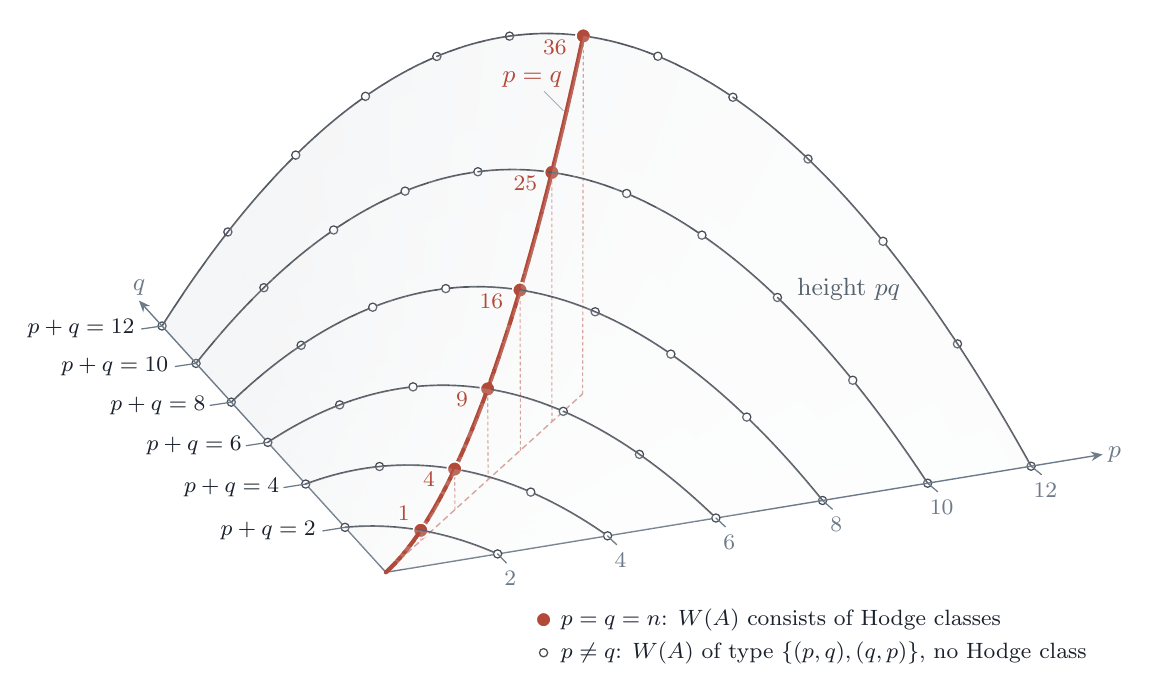
\begin{tikzpicture}[x=1cm,y=1cm,line join=round,line cap=round,
  font=\small,text=PInk]
  \node[circle,draw=PInk!80,fill=white,line width=0.45pt,inner sep=1.05pt] at (-5.0062,-0.7733) {};
  \draw[PSlate,line width=0.45pt] (-5.0062,-0.7733) -- (-5.2667,-0.8111);
  \draw[PInk!75,line width=0.6pt] (-5.0062,-0.7733) -- (-4.9278,-0.6506) -- (-4.8491,-0.5297);
  \path[draw=none,fill opacity=0.20,fill=PSlate!34!white] (-4.9353,-0.8514) -- (-5.0062,-0.7733) -- (-4.7307,-0.3519) -- (-4.6660,-0.4535) -- cycle;
  \draw[PInk!75,line width=0.6pt] (-4.8491,-0.5297) -- (-4.7702,-0.4107) -- (-4.6911,-0.2935);
  \draw[PInk!75,line width=0.6pt] (-4.6911,-0.2935) -- (-4.6117,-0.1783) -- (-4.5320,-0.0650);
  \path[draw=none,fill opacity=0.20,fill=PSlate!34!white] (-4.8639,-0.9299) -- (-4.9353,-0.8514) -- (-4.6660,-0.4535) -- (-4.6010,-0.5550) -- cycle;
  \path[draw=none,fill opacity=0.20,fill=PSlate!34!white] (-4.6660,-0.4535) -- (-4.7307,-0.3519) -- (-4.4521,0.0463) -- (-4.3939,-0.0778) -- cycle;
  \draw[PInk!75,line width=0.6pt] (-4.5320,-0.0650) -- (-4.4521,0.0463) -- (-4.3719,0.1558);
  \path[draw=none,fill opacity=0.20,fill=PSlate!34!white] (-4.7921,-1.0089) -- (-4.8639,-0.9299) -- (-4.6010,-0.5550) -- (-4.5357,-0.6563) -- cycle;
  \path[draw=none,fill opacity=0.20,fill=PSlate!34!white] (-4.6010,-0.5550) -- (-4.6660,-0.4535) -- (-4.3939,-0.0778) -- (-4.3354,-0.2012) -- cycle;
  \draw[PInk!75,line width=0.6pt] (-4.3719,0.1558) -- (-4.2915,0.2632) -- (-4.2109,0.3687);
  \path[draw=none,fill opacity=0.20,fill=PSlate!34!white] (-4.3939,-0.0778) -- (-4.4521,0.0463) -- (-4.1705,0.4208) -- (-4.1189,0.2752) -- cycle;
  \path[draw=none,fill opacity=0.20,fill=PSlate!34!white] (-4.7200,-1.0883) -- (-4.7921,-1.0089) -- (-4.5357,-0.6563) -- (-4.4700,-0.7575) -- cycle;
  \node[circle,draw=PInk!80,fill=white,line width=0.45pt,inner sep=1.05pt] at (-4.1705,0.4208) {};
  \path[draw=none,fill opacity=0.20,fill=PSlate!34!white] (-4.5357,-0.6563) -- (-4.6010,-0.5550) -- (-4.3354,-0.2012) -- (-4.2767,-0.3238) -- cycle;
  \draw[PInk!75,line width=0.6pt] (-4.2109,0.3687) -- (-4.1300,0.4723) -- (-4.0489,0.5738);
  \path[draw=none,fill opacity=0.20,fill=PSlate!34!white] (-4.3354,-0.2012) -- (-4.3939,-0.0778) -- (-4.1189,0.2752) -- (-4.0672,0.1310) -- cycle;
  \path[draw=none,fill opacity=0.20,fill=PSlate!34!white] (-4.6474,-1.1682) -- (-4.7200,-1.0883) -- (-4.4700,-0.7575) -- (-4.4040,-0.8584) -- cycle;
  \draw[PInk!75,line width=0.6pt] (-4.0489,0.5738) -- (-3.9675,0.6734) -- (-3.8859,0.7710);
  \path[draw=none,fill opacity=0.20,fill=PSlate!34!white] (-4.4700,-0.7575) -- (-4.5357,-0.6563) -- (-4.2767,-0.3238) -- (-4.2177,-0.4456) -- cycle;
  \path[draw=none,fill opacity=0.20,fill=PSlate!34!white] (-4.1189,0.2752) -- (-4.1705,0.4208) -- (-3.8859,0.7710) -- (-3.8412,0.6052) -- cycle;
  \path[draw=none,fill opacity=0.20,fill=PSlate!34!white] (-4.2767,-0.3238) -- (-4.3354,-0.2012) -- (-4.0672,0.1310) -- (-4.0152,-0.0118) -- cycle;
  \node[circle,draw=PInk!80,fill=white,line width=0.45pt,inner sep=1.05pt] at (-4.5743,-1.2486) {};
  \path[draw=none,fill opacity=0.20,fill=PSlate!34!white] (-4.5743,-1.2486) -- (-4.6474,-1.1682) -- (-4.4040,-0.8584) -- (-4.3376,-0.9592) -- cycle;
  \draw[PInk!75,line width=0.6pt] (-3.8859,0.7710) -- (-3.8041,0.8665) -- (-3.7220,0.9600);
  \path[draw=none,fill opacity=0.20,fill=PSlate!34!white] (-4.0672,0.1310) -- (-4.1189,0.2752) -- (-3.8412,0.6052) -- (-3.7964,0.4414) -- cycle;
  \draw[PSlate,line width=0.45pt] (-4.5743,-1.2486) -- (-4.8388,-1.2877);
  \path[draw=none,fill opacity=0.20,fill=PSlate!34!white] (-4.4040,-0.8584) -- (-4.4700,-0.7575) -- (-4.2177,-0.4456) -- (-4.1584,-0.5666) -- cycle;
  \draw[PInk!75,line width=0.6pt] (-4.5743,-1.2486) -- (-4.4934,-1.1475) -- (-4.4122,-1.0483);
  \path[draw=none,fill opacity=0.20,fill=PSlate!34!white] (-4.2177,-0.4456) -- (-4.2767,-0.3238) -- (-4.0152,-0.0118) -- (-3.9631,-0.1532) -- cycle;
  \path[draw=none,fill opacity=0.20,fill=PSlate!34!white] (-3.8412,0.6052) -- (-3.8859,0.7710) -- (-3.5985,1.0965) -- (-3.5609,0.9117) -- cycle;
  \draw[PInk!75,line width=0.6pt] (-3.7220,0.9600) -- (-3.6398,1.0515) -- (-3.5573,1.1410);
  \path[draw=none,fill opacity=0.20,fill=PSlate!34!white] (-4.0152,-0.0118) -- (-4.0672,0.1310) -- (-3.7964,0.4414) -- (-3.7514,0.2795) -- cycle;
  \path[draw=none,fill opacity=0.20,fill=PSlate!34!white] (-4.5009,-1.3294) -- (-4.5743,-1.2486) -- (-4.3376,-0.9592) -- (-4.2709,-1.0598) -- cycle;
  \draw[PInk!75,line width=0.6pt] (-4.4122,-1.0483) -- (-4.3308,-0.9512) -- (-4.2492,-0.8560);
  \path[draw=none,fill opacity=0.20,fill=PSlate!34!white] (-4.3376,-0.9592) -- (-4.4040,-0.8584) -- (-4.1584,-0.5666) -- (-4.0989,-0.6868) -- cycle;
  \path[draw=none,fill opacity=0.20,fill=PSlate!34!white] (-3.7964,0.4414) -- (-3.8412,0.6052) -- (-3.5609,0.9117) -- (-3.5231,0.7294) -- cycle;
  \path[draw=none,fill opacity=0.20,fill=PSlate!34!white] (-4.1584,-0.5666) -- (-4.2177,-0.4456) -- (-3.9631,-0.1532) -- (-3.9107,-0.2932) -- cycle;
  \draw[PInk!75,line width=0.6pt] (-3.5573,1.1410) -- (-3.4745,1.2284) -- (-3.3916,1.3137);
  \path[draw=none,fill opacity=0.20,fill=PSlate!34!white] (-3.9631,-0.1532) -- (-4.0152,-0.0118) -- (-3.7514,0.2795) -- (-3.7062,0.1196) -- cycle;
  \draw[PInk!75,line width=0.6pt] (-4.2492,-0.8560) -- (-4.1673,-0.7629) -- (-4.0852,-0.6718);
  \path[draw=none,fill opacity=0.20,fill=PSlate!34!white] (-3.5609,0.9117) -- (-3.5985,1.0965) -- (-3.3084,1.3969) -- (-3.2779,1.1944) -- cycle;
  \path[draw=none,fill opacity=0.20,fill=PSlate!34!white] (-4.4270,-1.4108) -- (-4.5009,-1.3294) -- (-4.2709,-1.0598) -- (-4.2038,-1.1603) -- cycle;
  \path[draw=none,fill opacity=0.20,fill=PSlate!34!white] (-4.2709,-1.0598) -- (-4.3376,-0.9592) -- (-4.0989,-0.6868) -- (-4.0390,-0.8062) -- cycle;
  \path[draw=none,fill opacity=0.20,fill=PSlate!34!white] (-3.7514,0.2795) -- (-3.7964,0.4414) -- (-3.5231,0.7294) -- (-3.4852,0.5497) -- cycle;
  \draw[PInk!75,line width=0.6pt] (-3.3916,1.3137) -- (-3.3084,1.3969) -- (-3.2250,1.4781);
  \node[circle,draw=PInk!80,fill=white,line width=0.45pt,inner sep=1.05pt] at (-3.3084,1.3969) {};
  \path[draw=none,fill opacity=0.20,fill=PSlate!34!white] (-4.0989,-0.6868) -- (-4.1584,-0.5666) -- (-3.9107,-0.2932) -- (-3.8581,-0.4317) -- cycle;
  \path[draw=none,fill opacity=0.20,fill=PSlate!34!white] (-3.9107,-0.2932) -- (-3.9631,-0.1532) -- (-3.7062,0.1196) -- (-3.6610,-0.0383) -- cycle;
  \draw[PInk!75,line width=0.6pt] (-4.0852,-0.6718) -- (-4.0028,-0.5827) -- (-3.9202,-0.4957);
  \path[draw=none,fill opacity=0.20,fill=PSlate!33!white] (-3.5231,0.7294) -- (-3.5609,0.9117) -- (-3.2779,1.1944) -- (-3.2474,0.9948) -- cycle;
  \path[draw=none,fill opacity=0.20,fill=PSlate!34!white] (-3.7062,0.1196) -- (-3.7514,0.2795) -- (-3.4852,0.5497) -- (-3.4473,0.3725) -- cycle;
  \draw[PInk!75,line width=0.6pt] (-3.2250,1.4781) -- (-3.1415,1.5572) -- (-3.0577,1.6341);
  \path[draw=none,fill opacity=0.20,fill=PSlate!34!white] (-4.3526,-1.4926) -- (-4.4270,-1.4108) -- (-4.2038,-1.1603) -- (-4.1364,-1.2605) -- cycle;
  \path[draw=none,fill opacity=0.20,fill=PSlate!34!white] (-4.2038,-1.1603) -- (-4.2709,-1.0598) -- (-4.0390,-0.8062) -- (-3.9789,-0.9248) -- cycle;
  \path[draw=none,fill opacity=0.20,fill=PSlate!33!white] (-3.2779,1.1944) -- (-3.3084,1.3969) -- (-3.0157,1.6718) -- (-2.9926,1.4528) -- cycle;
  \path[draw=none,fill opacity=0.20,fill=PSlate!34!white] (-4.0390,-0.8062) -- (-4.0989,-0.6868) -- (-3.8581,-0.4317) -- (-3.8054,-0.5689) -- cycle;
  \path[draw=none,fill opacity=0.20,fill=PSlate!33!white] (-3.4852,0.5497) -- (-3.5231,0.7294) -- (-3.2474,0.9948) -- (-3.2168,0.7984) -- cycle;
  \draw[PInk!75,line width=0.6pt] (-3.9202,-0.4957) -- (-3.8374,-0.4107) -- (-3.7544,-0.3278);
  \path[draw=none,fill opacity=0.20,fill=PSlate!34!white] (-3.8581,-0.4317) -- (-3.9107,-0.2932) -- (-3.6610,-0.0383) -- (-3.6155,-0.1942) -- cycle;
  \draw[PInk!75,line width=0.6pt] (-3.0577,1.6341) -- (-2.9737,1.7090) -- (-2.8895,1.7817);
  \path[draw=none,fill opacity=0.20,fill=PSlate!33!white] (-3.6610,-0.0383) -- (-3.7062,0.1196) -- (-3.4473,0.3725) -- (-3.4092,0.1978) -- cycle;
  \path[draw=none,fill opacity=0.20,fill=PSlate!33!white] (-3.2474,0.9948) -- (-3.2779,1.1944) -- (-2.9926,1.4528) -- (-2.9694,1.2373) -- cycle;
  \node[circle,draw=PInk!80,fill=white,line width=0.45pt,inner sep=1.05pt] at (-3.7128,-0.2871) {};
  \path[draw=none,fill opacity=0.20,fill=PSlate!34!white] (-4.1364,-1.2605) -- (-4.2038,-1.1603) -- (-3.9789,-0.9248) -- (-3.9185,-1.0426) -- cycle;
  \path[draw=none,fill opacity=0.20,fill=PSlate!34!white] (-4.2778,-1.5749) -- (-4.3526,-1.4926) -- (-4.1364,-1.2605) -- (-4.0685,-1.3606) -- cycle;
  \path[draw=none,fill opacity=0.20,fill=PSlate!33!white] (-3.4473,0.3725) -- (-3.4852,0.5497) -- (-3.2168,0.7984) -- (-3.1862,0.6050) -- cycle;
  \path[draw=none,fill opacity=0.20,fill=PSlate!34!white] (-3.9789,-0.9248) -- (-4.0390,-0.8062) -- (-3.8054,-0.5689) -- (-3.7524,-0.7047) -- cycle;
  \draw[PInk!75,line width=0.6pt] (-3.7544,-0.3278) -- (-3.6711,-0.2469) -- (-3.5877,-0.1681);
  \path[draw=none,fill opacity=0.20,fill=PSlate!34!white] (-3.8054,-0.5689) -- (-3.8581,-0.4317) -- (-3.6155,-0.1942) -- (-3.5699,-0.3480) -- cycle;
  \draw[PInk!75,line width=0.6pt] (-2.8895,1.7817) -- (-2.8051,1.8523) -- (-2.7204,1.9208);
  \path[draw=none,fill opacity=0.20,fill=PSlate!32!white] (-2.9926,1.4528) -- (-3.0157,1.6718) -- (-2.7204,1.9208) -- (-2.7048,1.6866) -- cycle;
  \path[draw=none,fill opacity=0.20,fill=PSlate!33!white] (-3.6155,-0.1942) -- (-3.6610,-0.0383) -- (-3.4092,0.1978) -- (-3.3710,0.0257) -- cycle;
  \path[draw=none,fill opacity=0.20,fill=PSlate!32!white] (-3.2168,0.7984) -- (-3.2474,0.9948) -- (-2.9694,1.2373) -- (-2.9463,1.0254) -- cycle;
  \path[draw=none,fill opacity=0.20,fill=PSlate!33!white] (-3.4092,0.1978) -- (-3.4473,0.3725) -- (-3.1862,0.6050) -- (-3.1555,0.4147) -- cycle;
  \draw[PInk!75,line width=0.6pt] (-3.5877,-0.1681) -- (-3.5040,-0.0914) -- (-3.4201,-0.0169);
  \path[draw=none,fill opacity=0.20,fill=PSlate!34!white] (-4.0685,-1.3606) -- (-4.1364,-1.2605) -- (-3.9185,-1.0426) -- (-3.8578,-1.1596) -- cycle;
  \path[draw=none,fill opacity=0.20,fill=PSlate!32!white] (-2.9694,1.2373) -- (-2.9926,1.4528) -- (-2.7048,1.6866) -- (-2.6893,1.4564) -- cycle;
  \path[draw=none,fill opacity=0.20,fill=PSlate!34!white] (-3.9185,-1.0426) -- (-3.9789,-0.9248) -- (-3.7524,-0.7047) -- (-3.6991,-0.8390) -- cycle;
  \draw[PInk!75,line width=0.6pt] (-2.7204,1.9208) -- (-2.6356,1.9871) -- (-2.5506,2.0513);
  \path[draw=none,fill opacity=0.20,fill=PSlate!34!white] (-4.2026,-1.6577) -- (-4.2778,-1.5749) -- (-4.0685,-1.3606) -- (-4.0004,-1.4606) -- cycle;
  \path[draw=none,fill opacity=0.20,fill=PSlate!33!white] (-3.7524,-0.7047) -- (-3.8054,-0.5689) -- (-3.5699,-0.3480) -- (-3.5242,-0.4999) -- cycle;
  \path[draw=none,fill opacity=0.20,fill=PSlate!32!white] (-3.1862,0.6050) -- (-3.2168,0.7984) -- (-2.9463,1.0254) -- (-2.9231,0.8171) -- cycle;
  \path[draw=none,fill opacity=0.20,fill=PSlate!33!white] (-3.5699,-0.3480) -- (-3.6155,-0.1942) -- (-3.3710,0.0257) -- (-3.3328,-0.1439) -- cycle;
  \path[draw=none,fill opacity=0.20,fill=PSlate!32!white] (-3.3710,0.0257) -- (-3.4092,0.1978) -- (-3.1555,0.4147) -- (-3.1248,0.2275) -- cycle;
  \path[draw=none,fill opacity=0.20,fill=PSlate!31!white] (-2.7048,1.6866) -- (-2.7204,1.9208) -- (-2.4228,2.1434) -- (-2.4149,1.8955) -- cycle;
  \draw[PInk!75,line width=0.6pt] (-3.4201,-0.0169) -- (-3.3360,0.0556) -- (-3.2516,0.1260);
  \path[draw=none,fill opacity=0.20,fill=PSlate!31!white] (-2.9463,1.0254) -- (-2.9694,1.2373) -- (-2.6893,1.4564) -- (-2.6737,1.2303) -- cycle;
  \draw[PInk!75,line width=0.6pt] (-2.5506,2.0513) -- (-2.4655,2.1133) -- (-2.3801,2.1731);
  \node[circle,draw=PInk!80,fill=white,line width=0.45pt,inner sep=1.05pt] at (-2.4228,2.1434) {};
  \path[draw=none,fill opacity=0.20,fill=PSlate!32!white] (-3.1555,0.4147) -- (-3.1862,0.6050) -- (-2.9231,0.8171) -- (-2.9000,0.6123) -- cycle;
  \path[draw=none,fill opacity=0.20,fill=PSlate!33!white] (-3.8578,-1.1596) -- (-3.9185,-1.0426) -- (-3.6991,-0.8390) -- (-3.6457,-0.9719) -- cycle;
  \path[draw=none,fill opacity=0.20,fill=PSlate!34!white] (-4.0004,-1.4606) -- (-4.0685,-1.3606) -- (-3.8578,-1.1596) -- (-3.7968,-1.2757) -- cycle;
  \path[draw=none,fill opacity=0.20,fill=PSlate!33!white] (-3.6991,-0.8390) -- (-3.7524,-0.7047) -- (-3.5242,-0.4999) -- (-3.4782,-0.6498) -- cycle;
  \path[draw=none,fill opacity=0.20,fill=PSlate!34!white] (-4.1269,-1.7410) -- (-4.2026,-1.6577) -- (-4.0004,-1.4606) -- (-3.9318,-1.5603) -- cycle;
  \path[draw=none,fill opacity=0.20,fill=PSlate!32!white] (-3.5242,-0.4999) -- (-3.5699,-0.3480) -- (-3.3328,-0.1439) -- (-3.2944,-0.3108) -- cycle;
  \path[draw=none,fill opacity=0.20,fill=PSlate!31!white] (-2.6893,1.4564) -- (-2.7048,1.6866) -- (-2.4149,1.8955) -- (-2.4070,1.6520) -- cycle;
  \node[circle,draw=PInk!80,fill=white,line width=0.45pt,inner sep=1.05pt] at (-4.1269,-1.7410) {};
  \path[draw=none,fill opacity=0.20,fill=PSlate!31!white] (-2.9231,0.8171) -- (-2.9463,1.0254) -- (-2.6737,1.2303) -- (-2.6582,1.0083) -- cycle;
  \draw[PInk!75,line width=0.6pt] (-3.2516,0.1260) -- (-3.1671,0.1942) -- (-3.0824,0.2603);
  \path[draw=none,fill opacity=0.20,fill=PSlate!32!white] (-3.3328,-0.1439) -- (-3.3710,0.0257) -- (-3.1248,0.2275) -- (-3.0940,0.0434) -- cycle;
  \draw[PInk!75,line width=0.6pt] (-2.3801,2.1731) -- (-2.2945,2.2307) -- (-2.2088,2.2862);
  \draw[PSlate,line width=0.45pt] (-4.1269,-1.7410) -- (-4.3955,-1.7815);
  \draw[PInk!75,line width=0.6pt] (-4.1269,-1.7410) -- (-4.0435,-1.6622) -- (-3.9598,-1.5854);
  \path[draw=none,fill opacity=0.20,fill=PSlate!31!white] (-3.1248,0.2275) -- (-3.1555,0.4147) -- (-2.9000,0.6123) -- (-2.8768,0.4112) -- cycle;
  \path[draw=none,fill opacity=0.20,fill=PSlate!30!white] (-2.4149,1.8955) -- (-2.4228,2.1434) -- (-2.1229,2.3394) -- (-2.1227,2.0790) -- cycle;
  \path[draw=none,fill opacity=0.20,fill=PSlate!30!white] (-2.6737,1.2303) -- (-2.6893,1.4564) -- (-2.4070,1.6520) -- (-2.3991,1.4130) -- cycle;
  \path[draw=none,fill opacity=0.20,fill=PSlate!33!white] (-3.6457,-0.9719) -- (-3.6991,-0.8390) -- (-3.4782,-0.6498) -- (-3.4322,-0.7977) -- cycle;
  \path[draw=none,fill opacity=0.20,fill=PSlate!33!white] (-3.7968,-1.2757) -- (-3.8578,-1.1596) -- (-3.6457,-0.9719) -- (-3.5920,-1.1033) -- cycle;
  \path[draw=none,fill opacity=0.20,fill=PSlate!31!white] (-2.9000,0.6123) -- (-2.9231,0.8171) -- (-2.6582,1.0083) -- (-2.6426,0.7903) -- cycle;
  \path[draw=none,fill opacity=0.20,fill=PSlate!32!white] (-3.4782,-0.6498) -- (-3.5242,-0.4999) -- (-3.2944,-0.3108) -- (-3.2559,-0.4753) -- cycle;
  \draw[PInk!75,line width=0.6pt] (-3.0824,0.2603) -- (-2.9974,0.3243) -- (-2.9123,0.3861);
  \path[draw=none,fill opacity=0.20,fill=PSlate!33!white] (-3.9318,-1.5603) -- (-4.0004,-1.4606) -- (-3.7968,-1.2757) -- (-3.7355,-1.3911) -- cycle;
  \draw[PInk!75,line width=0.6pt] (-2.2088,2.2862) -- (-2.1229,2.3394) -- (-2.0368,2.3905);
  \path[draw=none,fill opacity=0.20,fill=PSlate!32!white] (-3.2944,-0.3108) -- (-3.3328,-0.1439) -- (-3.0940,0.0434) -- (-3.0631,-0.1376) -- cycle;
  \path[draw=none,fill opacity=0.20,fill=PSlate!34!white] (-4.0508,-1.8247) -- (-4.1269,-1.7410) -- (-3.9318,-1.5603) -- (-3.8629,-1.6599) -- cycle;
  \path[draw=none,fill opacity=0.20,fill=PSlate!30!white] (-2.4070,1.6520) -- (-2.4149,1.8955) -- (-2.1227,2.0790) -- (-2.1227,1.8236) -- cycle;
  \draw[PInk!75,line width=0.6pt] (-3.9598,-1.5854) -- (-3.8759,-1.5108) -- (-3.7917,-1.4383);
  \path[draw=none,fill opacity=0.20,fill=PSlate!31!white] (-3.0940,0.0434) -- (-3.1248,0.2275) -- (-2.8768,0.4112) -- (-2.8536,0.2136) -- cycle;
  \path[draw=none,fill opacity=0.20,fill=PSlate!30!white] (-2.6582,1.0083) -- (-2.6737,1.2303) -- (-2.3991,1.4130) -- (-2.3914,1.1785) -- cycle;
  \path[draw=none,fill opacity=0.20,fill=PSlate!30!white] (-2.8768,0.4112) -- (-2.9000,0.6123) -- (-2.6426,0.7903) -- (-2.6271,0.5764) -- cycle;
  \draw[PInk!75,line width=0.6pt] (-2.0368,2.3905) -- (-1.9505,2.4393) -- (-1.8640,2.4859);
  \draw[PInk!75,line width=0.6pt] (-2.9123,0.3861) -- (-2.8270,0.4457) -- (-2.7415,0.5032);
  \node[circle,draw=PInk!80,fill=white,line width=0.45pt,inner sep=1.05pt] at (-2.8270,0.4457) {};
  \path[draw=none,fill opacity=0.20,fill=PSlate!29!white] (-2.3991,1.4130) -- (-2.4070,1.6520) -- (-2.1227,1.8236) -- (-2.1227,1.5730) -- cycle;
  \path[draw=none,fill opacity=0.20,fill=PSlate!29!white] (-2.1227,2.0790) -- (-2.1229,2.3394) -- (-1.8208,2.5084) -- (-1.8286,2.2370) -- cycle;
  \path[draw=none,fill opacity=0.20,fill=PSlate!32!white] (-3.5920,-1.1033) -- (-3.6457,-0.9719) -- (-3.4322,-0.7977) -- (-3.3859,-0.9435) -- cycle;
  \path[draw=none,fill opacity=0.20,fill=PSlate!32!white] (-3.4322,-0.7977) -- (-3.4782,-0.6498) -- (-3.2559,-0.4753) -- (-3.2173,-0.6371) -- cycle;
  \path[draw=none,fill opacity=0.20,fill=PSlate!33!white] (-3.7355,-1.3911) -- (-3.7968,-1.2757) -- (-3.5920,-1.1033) -- (-3.5381,-1.2334) -- cycle;
  \path[draw=none,fill opacity=0.20,fill=PSlate!31!white] (-3.2559,-0.4753) -- (-3.2944,-0.3108) -- (-3.0631,-0.1376) -- (-3.0322,-0.3155) -- cycle;
  \path[draw=none,fill opacity=0.20,fill=PSlate!30!white] (-2.6426,0.7903) -- (-2.6582,1.0083) -- (-2.3914,1.1785) -- (-2.3836,0.9485) -- cycle;
  \path[draw=none,fill opacity=0.20,fill=PSlate!33!white] (-3.8629,-1.6599) -- (-3.9318,-1.5603) -- (-3.7355,-1.3911) -- (-3.6740,-1.5056) -- cycle;
  \draw[PInk!75,line width=0.6pt] (-3.7917,-1.4383) -- (-3.7074,-1.3678) -- (-3.6229,-1.2995);
  \path[draw=none,fill opacity=0.20,fill=PSlate!31!white] (-3.0631,-0.1376) -- (-3.0940,0.0434) -- (-2.8536,0.2136) -- (-2.8304,0.0197) -- cycle;
  \draw[PInk!75,line width=0.6pt] (-1.8640,2.4859) -- (-1.7774,2.5303) -- (-1.6906,2.5724);
  \path[draw=none,fill opacity=0.20,fill=PSlate!33!white] (-3.9742,-1.9090) -- (-4.0508,-1.8247) -- (-3.8629,-1.6599) -- (-3.7936,-1.7593) -- cycle;
  \path[draw=none,fill opacity=0.20,fill=PSlate!30!white] (-2.8536,0.2136) -- (-2.8768,0.4112) -- (-2.6271,0.5764) -- (-2.6117,0.3666) -- cycle;
  \path[draw=none,fill opacity=0.20,fill=PSlate!28!white] (-2.1227,1.8236) -- (-2.1227,2.0790) -- (-1.8286,2.2370) -- (-1.8365,1.9710) -- cycle;
  \draw[PInk!75,line width=0.6pt] (-2.7415,0.5032) -- (-2.6558,0.5585) -- (-2.5699,0.6116);
  \path[draw=none,fill opacity=0.20,fill=PSlate!29!white] (-2.3914,1.1785) -- (-2.3991,1.4130) -- (-2.1227,1.5730) -- (-2.1228,1.3274) -- cycle;
  \path[draw=none,fill opacity=0.20,fill=PSlate!29!white] (-2.6271,0.5764) -- (-2.6426,0.7903) -- (-2.3836,0.9485) -- (-2.3759,0.7230) -- cycle;
  \path[draw=none,fill opacity=0.20,fill=PSlate!31!white] (-3.3859,-0.9435) -- (-3.4322,-0.7977) -- (-3.2173,-0.6371) -- (-3.1786,-0.7963) -- cycle;
  \path[draw=none,fill opacity=0.20,fill=PSlate!31!white] (-3.2173,-0.6371) -- (-3.2559,-0.4753) -- (-3.0322,-0.3155) -- (-3.0012,-0.4903) -- cycle;
  \path[draw=none,fill opacity=0.20,fill=PSlate!32!white] (-3.5381,-1.2334) -- (-3.5920,-1.1033) -- (-3.3859,-0.9435) -- (-3.3395,-1.0873) -- cycle;
  \draw[PInk!75,line width=0.6pt] (-3.6229,-1.2995) -- (-3.5381,-1.2334) -- (-3.4531,-1.1693);
  \path[draw=none,fill opacity=0.20,fill=PSlate!28!white] (-2.1227,1.5730) -- (-2.1227,1.8236) -- (-1.8365,1.9710) -- (-1.8445,1.7102) -- cycle;
  \path[draw=none,fill opacity=0.20,fill=PSlate!30!white] (-3.0322,-0.3155) -- (-3.0631,-0.1376) -- (-2.8304,0.0197) -- (-2.8071,-0.1706) -- cycle;
  \path[draw=none,fill opacity=0.20,fill=PSlate!28!white] (-1.8286,2.2370) -- (-1.8208,2.5084) -- (-1.5166,2.6500) -- (-1.5325,2.3691) -- cycle;
  \draw[PInk!75,line width=0.6pt] (-1.6906,2.5724) -- (-1.6037,2.6123) -- (-1.5166,2.6500);
  \path[draw=none,fill opacity=0.20,fill=PSlate!32!white] (-3.6740,-1.5056) -- (-3.7355,-1.3911) -- (-3.5381,-1.2334) -- (-3.4839,-1.3619) -- cycle;
  \path[draw=none,fill opacity=0.20,fill=PSlate!29!white] (-2.3836,0.9485) -- (-2.3914,1.1785) -- (-2.1228,1.3274) -- (-2.1230,1.0867) -- cycle;
  \draw[PInk!75,line width=0.6pt] (-2.5699,0.6116) -- (-2.4838,0.6625) -- (-2.3975,0.7112);
  \path[draw=none,fill opacity=0.20,fill=PSlate!30!white] (-2.8304,0.0197) -- (-2.8536,0.2136) -- (-2.6117,0.3666) -- (-2.5962,0.1608) -- cycle;
  \path[draw=none,fill opacity=0.20,fill=PSlate!32!white] (-3.7936,-1.7593) -- (-3.8629,-1.6599) -- (-3.6740,-1.5056) -- (-3.6121,-1.6193) -- cycle;
  \node[circle,draw=PInk!80,fill=white,line width=0.45pt,inner sep=1.05pt] at (-1.5166,2.6500) {};
  \path[draw=none,fill opacity=0.20,fill=PSlate!29!white] (-2.6117,0.3666) -- (-2.6271,0.5764) -- (-2.3759,0.7230) -- (-2.3683,0.5021) -- cycle;
  \path[draw=none,fill opacity=0.20,fill=PSlate!27!white] (-1.8365,1.9710) -- (-1.8286,2.2370) -- (-1.5325,2.3691) -- (-1.5485,2.0940) -- cycle;
  \path[draw=none,fill opacity=0.20,fill=PSlate!28!white] (-2.1228,1.3274) -- (-2.1227,1.5730) -- (-1.8445,1.7102) -- (-1.8526,1.4548) -- cycle;
  \path[draw=none,fill opacity=0.20,fill=PSlate!33!white] (-3.8971,-1.9939) -- (-3.9742,-1.9090) -- (-3.7936,-1.7593) -- (-3.7239,-1.8585) -- cycle;
  \draw[PInk!75,line width=0.6pt] (-1.5166,2.6500) -- (-1.4293,2.6854) -- (-1.3419,2.7185);
  \draw[PClay!60,line width=0.4pt,dash pattern=on 1pt off 1.2pt] (0.3352,-1.6351) -- (0.3439,2.9102);
  \draw[PInk!75,line width=0.6pt] (-3.4531,-1.1693) -- (-3.3679,-1.1074) -- (-3.2825,-1.0477);
  \path[draw=none,fill opacity=0.20,fill=PSlate!28!white] (-2.3759,0.7230) -- (-2.3836,0.9485) -- (-2.1230,1.0867) -- (-2.1232,0.8509) -- cycle;
  \path[draw=none,fill opacity=0.20,fill=PSlate!30!white] (-3.1786,-0.7963) -- (-3.2173,-0.6371) -- (-3.0012,-0.4903) -- (-2.9701,-0.6619) -- cycle;
  \path[draw=none,fill opacity=0.20,fill=PSlate!31!white] (-3.3395,-1.0873) -- (-3.3859,-0.9435) -- (-3.1786,-0.7963) -- (-3.1398,-0.9529) -- cycle;
  \path[draw=none,fill opacity=0.20,fill=PSlate!30!white] (-3.0012,-0.4903) -- (-3.0322,-0.3155) -- (-2.8071,-0.1706) -- (-2.7838,-0.3573) -- cycle;
  \draw[PInk!75,line width=0.6pt] (-2.3975,0.7112) -- (-2.3111,0.7577) -- (-2.2245,0.8020);
  \path[draw=none,fill opacity=0.20,fill=PSlate!31!white] (-3.4839,-1.3619) -- (-3.5381,-1.2334) -- (-3.3395,-1.0873) -- (-3.2929,-1.2290) -- cycle;
  \path[draw=none,fill opacity=0.20,fill=PSlate!29!white] (-2.8071,-0.1706) -- (-2.8304,0.0197) -- (-2.5962,0.1608) -- (-2.5807,-0.0409) -- cycle;
  \path[draw=none,fill opacity=0.20,fill=PSlate!27!white] (-1.8445,1.7102) -- (-1.8365,1.9710) -- (-1.5485,2.0940) -- (-1.5646,1.8244) -- cycle;
  \path[draw=none,fill opacity=0.20,fill=PSlate!32!white] (-3.6121,-1.6193) -- (-3.6740,-1.5056) -- (-3.4839,-1.3619) -- (-3.4295,-1.4891) -- cycle;
  \path[draw=none,fill opacity=0.20,fill=PSlate!27!white] (-1.5325,2.3691) -- (-1.5166,2.6500) -- (-1.2105,2.7639) -- (-1.2346,2.4751) -- cycle;
  \path[draw=none,fill opacity=0.20,fill=PSlate!28!white] (-2.1230,1.0867) -- (-2.1228,1.3274) -- (-1.8526,1.4548) -- (-1.8607,1.2046) -- cycle;
  \path[draw=none,fill opacity=0.20,fill=PSlate!29!white] (-2.5962,0.1608) -- (-2.6117,0.3666) -- (-2.3683,0.5021) -- (-2.3607,0.2856) -- cycle;
  \draw[PInk!75,line width=0.6pt] (-1.3419,2.7185) -- (-1.2544,2.7493) -- (-1.1667,2.7779);
  \node[circle,draw=PInk!80,fill=white,line width=0.45pt,inner sep=1.05pt] at (-3.2398,-1.0186) {};
  \path[draw=none,fill opacity=0.20,fill=PSlate!32!white] (-3.7239,-1.8585) -- (-3.7936,-1.7593) -- (-3.6121,-1.6193) -- (-3.5498,-1.7321) -- cycle;
  \path[draw=none,fill opacity=0.20,fill=PSlate!28!white] (-2.3683,0.5021) -- (-2.3759,0.7230) -- (-2.1232,0.8509) -- (-2.1235,0.6200) -- cycle;
  \draw[PInk!75,line width=0.6pt] (-3.2825,-1.0477) -- (-3.1970,-0.9901) -- (-3.1112,-0.9347);
  \draw[PInk!75,line width=0.6pt] (-2.2245,0.8020) -- (-2.1377,0.8441) -- (-2.0507,0.8839);
  \path[draw=none,fill opacity=0.20,fill=PSlate!26!white] (-1.5485,2.0940) -- (-1.5325,2.3691) -- (-1.2346,2.4751) -- (-1.2588,2.1922) -- cycle;
  \path[draw=none,fill opacity=0.20,fill=PSlate!27!white] (-1.8526,1.4548) -- (-1.8445,1.7102) -- (-1.5646,1.8244) -- (-1.5808,1.5604) -- cycle;
  \path[draw=none,fill opacity=0.20,fill=PSlate!30!white] (-2.9701,-0.6619) -- (-3.0012,-0.4903) -- (-2.7838,-0.3573) -- (-2.7605,-0.5404) -- cycle;
  \path[draw=none,fill opacity=0.20,fill=PSlate!30!white] (-3.1398,-0.9529) -- (-3.1786,-0.7963) -- (-2.9701,-0.6619) -- (-2.9390,-0.8304) -- cycle;
  \path[draw=none,fill opacity=0.20,fill=PSlate!29!white] (-2.7838,-0.3573) -- (-2.8071,-0.1706) -- (-2.5807,-0.0409) -- (-2.5653,-0.2385) -- cycle;
  \path[draw=none,fill opacity=0.20,fill=PSlate!27!white] (-2.1232,0.8509) -- (-2.1230,1.0867) -- (-1.8607,1.2046) -- (-1.8690,0.9597) -- cycle;
  \path[draw=none,fill opacity=0.20,fill=PSlate!32!white] (-3.8196,-2.0792) -- (-3.8971,-1.9939) -- (-3.7239,-1.8585) -- (-3.6538,-1.9576) -- cycle;
  \path[draw=none,fill opacity=0.20,fill=PSlate!30!white] (-3.2929,-1.2290) -- (-3.3395,-1.0873) -- (-3.1398,-0.9529) -- (-3.1008,-1.1070) -- cycle;
  \draw[PSlate,line width=0.5pt,-{Stealth[length=4.2pt,width=3.4pt]}] (-2.1637,-3.9015) -- (-5.2997,-0.4504);
  \draw[PInk!75,line width=0.6pt] (-1.1667,2.7779) -- (-1.0788,2.8042) -- (-0.9908,2.8282);
  \path[draw=none,fill opacity=0.20,fill=PSlate!28!white] (-2.5807,-0.0409) -- (-2.5962,0.1608) -- (-2.3607,0.2856) -- (-2.3531,0.0737) -- cycle;
  \path[draw=none,fill opacity=0.20,fill=PSlate!31!white] (-3.4295,-1.4891) -- (-3.4839,-1.3619) -- (-3.2929,-1.2290) -- (-3.2461,-1.3687) -- cycle;
  \path[draw=none,fill opacity=0.20,fill=PSlate!26!white] (-1.5646,1.8244) -- (-1.5485,2.0940) -- (-1.2588,2.1922) -- (-1.2831,1.9152) -- cycle;
  \path[draw=none,fill opacity=0.20,fill=PSlate!28!white] (-2.3607,0.2856) -- (-2.3683,0.5021) -- (-2.1235,0.6200) -- (-2.1238,0.3940) -- cycle;
  \path[draw=none,fill opacity=0.20,fill=PSlate!27!white] (-1.8607,1.2046) -- (-1.8526,1.4548) -- (-1.5808,1.5604) -- (-1.5971,1.3021) -- cycle;
  \path[draw=none,fill opacity=0.20,fill=PSlate!25!white] (-1.2346,2.4751) -- (-1.2105,2.7639) -- (-0.9027,2.8499) -- (-0.9351,2.5547) -- cycle;
  \draw[PInk!75,line width=0.6pt] (-2.0507,0.8839) -- (-1.9636,0.9215) -- (-1.8763,0.9568);
  \path[draw=none,fill opacity=0.20,fill=PSlate!31!white] (-3.5498,-1.7321) -- (-3.6121,-1.6193) -- (-3.4295,-1.4891) -- (-3.3749,-1.6147) -- cycle;
  \draw[PInk!75,line width=0.6pt] (-3.1112,-0.9347) -- (-3.0252,-0.8815) -- (-2.9390,-0.8304);
  \node[circle,draw=PInk!80,fill=white,line width=0.45pt,inner sep=1.05pt] at (-1.9199,0.9395) {};
  \path[draw=none,fill opacity=0.20,fill=PSlate!27!white] (-2.1235,0.6200) -- (-2.1232,0.8509) -- (-1.8690,0.9597) -- (-1.8773,0.7201) -- cycle;
  \draw[PInk!75,line width=0.6pt] (-0.9908,2.8282) -- (-0.9027,2.8499) -- (-0.8144,2.8694);
  \path[draw=none,fill opacity=0.20,fill=PSlate!31!white] (-3.6538,-1.9576) -- (-3.7239,-1.8585) -- (-3.5498,-1.7321) -- (-3.4873,-1.8441) -- cycle;
  \path[draw=none,fill opacity=0.20,fill=PSlate!29!white] (-2.9390,-0.8304) -- (-2.9701,-0.6619) -- (-2.7605,-0.5404) -- (-2.7372,-0.7199) -- cycle;
  \path[draw=none,fill opacity=0.20,fill=PSlate!29!white] (-2.7605,-0.5404) -- (-2.7838,-0.3573) -- (-2.5653,-0.2385) -- (-2.5498,-0.4320) -- cycle;
  \path[draw=none,fill opacity=0.20,fill=PSlate!26!white] (-1.5808,1.5604) -- (-1.5646,1.8244) -- (-1.2831,1.9152) -- (-1.3075,1.6442) -- cycle;
  \path[draw=none,fill opacity=0.20,fill=PSlate!25!white] (-1.2588,2.1922) -- (-1.2346,2.4751) -- (-0.9351,2.5547) -- (-0.9675,2.2655) -- cycle;
  \path[draw=none,fill opacity=0.20,fill=PSlate!30!white] (-3.1008,-1.1070) -- (-3.1398,-0.9529) -- (-2.9390,-0.8304) -- (-2.9078,-0.9958) -- cycle;
  \path[draw=none,fill opacity=0.20,fill=PSlate!28!white] (-2.5653,-0.2385) -- (-2.5807,-0.0409) -- (-2.3531,0.0737) -- (-2.3456,-0.1337) -- cycle;
  \path[draw=none,fill opacity=0.20,fill=PSlate!26!white] (-1.8690,0.9597) -- (-1.8607,1.2046) -- (-1.5971,1.3021) -- (-1.6134,1.0494) -- cycle;
  \path[draw=none,fill opacity=0.20,fill=PSlate!30!white] (-3.2461,-1.3687) -- (-3.2929,-1.2290) -- (-3.1008,-1.1070) -- (-3.0618,-1.2584) -- cycle;
  \path[draw=none,fill opacity=0.20,fill=PSlate!27!white] (-2.3531,0.0737) -- (-2.3607,0.2856) -- (-2.1238,0.3940) -- (-2.1243,0.1729) -- cycle;
  \draw[PInk!75,line width=0.6pt] (-1.8763,0.9568) -- (-1.7888,0.9899) -- (-1.7012,1.0208);
  \draw[PInk!75,line width=0.6pt] (-2.9390,-0.8304) -- (-2.8526,-0.7816) -- (-2.7661,-0.7349);
  \path[draw=none,fill opacity=0.20,fill=PSlate!31!white] (-3.7416,-2.1650) -- (-3.8196,-2.0792) -- (-3.6538,-1.9576) -- (-3.5834,-2.0565) -- cycle;
  \path[draw=none,fill opacity=0.20,fill=PSlate!30!white] (-3.3749,-1.6147) -- (-3.4295,-1.4891) -- (-3.2461,-1.3687) -- (-3.1991,-1.5063) -- cycle;
  \draw[PInk!75,line width=0.6pt] (-0.8144,2.8694) -- (-0.7260,2.8865) -- (-0.6375,2.9013);
  \path[draw=none,fill opacity=0.20,fill=PSlate!27!white] (-2.1238,0.3940) -- (-2.1235,0.6200) -- (-1.8773,0.7201) -- (-1.8858,0.4857) -- cycle;
  \path[draw=none,fill opacity=0.20,fill=PSlate!25!white] (-1.2831,1.9152) -- (-1.2588,2.1922) -- (-0.9675,2.2655) -- (-1.0001,1.9826) -- cycle;
  \path[draw=none,fill opacity=0.20,fill=PSlate!26!white] (-1.5971,1.3021) -- (-1.5808,1.5604) -- (-1.3075,1.6442) -- (-1.3320,1.3790) -- cycle;
  \path[draw=none,fill opacity=0.20,fill=PSlate!24!white] (-0.9351,2.5547) -- (-0.9027,2.8499) -- (-0.5932,2.9078) -- (-0.6339,2.6076) -- cycle;
  \path[draw=none,fill opacity=0.20,fill=PSlate!26!white] (-1.8773,0.7201) -- (-1.8690,0.9597) -- (-1.6134,1.0494) -- (-1.6299,0.8022) -- cycle;
  \path[draw=none,fill opacity=0.20,fill=PSlate!31!white] (-3.4873,-1.8441) -- (-3.5498,-1.7321) -- (-3.3749,-1.6147) -- (-3.3200,-1.7389) -- cycle;
  \path[draw=none,fill opacity=0.20,fill=PSlate!28!white] (-2.7372,-0.7199) -- (-2.7605,-0.5404) -- (-2.5498,-0.4320) -- (-2.5344,-0.6214) -- cycle;
  \path[draw=none,fill opacity=0.20,fill=PSlate!28!white] (-2.5498,-0.4320) -- (-2.5653,-0.2385) -- (-2.3456,-0.1337) -- (-2.3381,-0.3366) -- cycle;
  \node[circle,draw=PInk!80,fill=white,line width=0.45pt,inner sep=1.05pt] at (-0.5932,2.9078) {};
  \path[draw=none,fill opacity=0.20,fill=PSlate!29!white] (-2.9078,-0.9958) -- (-2.9390,-0.8304) -- (-2.7372,-0.7199) -- (-2.7138,-0.8957) -- cycle;
  \draw[PInk!75,line width=0.6pt] (-1.7012,1.0208) -- (-1.6134,1.0494) -- (-1.5255,1.0757);
  \path[draw=none,fill opacity=0.20,fill=PSlate!25!white] (-1.3075,1.6442) -- (-1.2831,1.9152) -- (-1.0001,1.9826) -- (-1.0328,1.7058) -- cycle;
  \path[draw=none,fill opacity=0.20,fill=PSlate!27!white] (-2.3456,-0.1337) -- (-2.3531,0.0737) -- (-2.1243,0.1729) -- (-2.1248,-0.0433) -- cycle;
  \path[draw=none,fill opacity=0.20,fill=PSlate!24!white] (-0.9675,2.2655) -- (-0.9351,2.5547) -- (-0.6339,2.6076) -- (-0.6748,2.3137) -- cycle;
  \path[draw=none,fill opacity=0.20,fill=PSlate!29!white] (-3.0618,-1.2584) -- (-3.1008,-1.1070) -- (-2.9078,-0.9958) -- (-2.8765,-1.1580) -- cycle;
  \draw[PInk!75,line width=0.6pt] (-0.6375,2.9013) -- (-0.5489,2.9138) -- (-0.4601,2.9239);
  \path[draw=none,fill opacity=0.20,fill=PSlate!25!white] (-1.6134,1.0494) -- (-1.5971,1.3021) -- (-1.3320,1.3790) -- (-1.3566,1.1197) -- cycle;
  \draw[PInk!75,line width=0.6pt] (-2.7661,-0.7349) -- (-2.6794,-0.6905) -- (-2.5924,-0.6483);
  \path[draw=none,fill opacity=0.20,fill=PSlate!26!white] (-2.1243,0.1729) -- (-2.1238,0.3940) -- (-1.8858,0.4857) -- (-1.8943,0.2566) -- cycle;
  \path[draw=none,fill opacity=0.20,fill=PSlate!31!white] (-3.5834,-2.0565) -- (-3.6538,-1.9576) -- (-3.4873,-1.8441) -- (-3.4245,-1.9553) -- cycle;
  \path[draw=none,fill opacity=0.20,fill=PSlate!29!white] (-3.1991,-1.5063) -- (-3.2461,-1.3687) -- (-3.0618,-1.2584) -- (-3.0226,-1.4071) -- cycle;
  \path[draw=none,fill opacity=0.20,fill=PSlate!26!white] (-1.8858,0.4857) -- (-1.8773,0.7201) -- (-1.6299,0.8022) -- (-1.6465,0.5607) -- cycle;
  \path[draw=none,fill opacity=0.20,fill=PSlate!24!white] (-1.0001,1.9826) -- (-0.9675,2.2655) -- (-0.6748,2.3137) -- (-0.7158,2.0263) -- cycle;
  \path[draw=none,fill opacity=0.20,fill=PSlate!24!white] (-1.3320,1.3790) -- (-1.3075,1.6442) -- (-1.0328,1.7058) -- (-1.0656,1.4352) -- cycle;
  \path[draw=none,fill opacity=0.20,fill=PSlate!30!white] (-3.3200,-1.7389) -- (-3.3749,-1.6147) -- (-3.1991,-1.5063) -- (-3.1520,-1.6419) -- cycle;
  \draw[PInk!75,line width=0.6pt] (-1.5255,1.0757) -- (-1.4375,1.0997) -- (-1.3492,1.1215);
  \path[draw=none,fill opacity=0.20,fill=PSlate!23!white] (-0.6339,2.6076) -- (-0.5932,2.9078) -- (-0.2822,2.9373) -- (-0.3314,2.6337) -- cycle;
  \draw[PInk!75,line width=0.6pt] (-0.4601,2.9239) -- (-0.3712,2.9318) -- (-0.2822,2.9373);
  \path[draw=none,fill opacity=0.20,fill=PSlate!25!white] (-1.6299,0.8022) -- (-1.6134,1.0494) -- (-1.3566,1.1197) -- (-1.3813,0.8663) -- cycle;
  \path[draw=none,fill opacity=0.20,fill=PSlate!27!white] (-2.5344,-0.6214) -- (-2.5498,-0.4320) -- (-2.3381,-0.3366) -- (-2.3306,-0.5350) -- cycle;
  \path[draw=none,fill opacity=0.20,fill=PSlate!31!white] (-3.6631,-2.2514) -- (-3.7416,-2.1650) -- (-3.5834,-2.0565) -- (-3.5125,-2.1552) -- cycle;
  \path[draw=none,fill opacity=0.20,fill=PSlate!28!white] (-2.7138,-0.8957) -- (-2.7372,-0.7199) -- (-2.5344,-0.6214) -- (-2.5190,-0.8066) -- cycle;
  \path[draw=none,fill opacity=0.20,fill=PSlate!27!white] (-2.3381,-0.3366) -- (-2.3456,-0.1337) -- (-2.1248,-0.0433) -- (-2.1253,-0.2545) -- cycle;
  \draw[PInk!75,line width=0.6pt] (-2.5924,-0.6483) -- (-2.5054,-0.6083) -- (-2.4181,-0.5705);
  \path[draw=none,fill opacity=0.20,fill=PSlate!28!white] (-2.8765,-1.1580) -- (-2.9078,-0.9958) -- (-2.7138,-0.8957) -- (-2.6905,-1.0678) -- cycle;
  \draw[PClay!60,line width=0.4pt,dash pattern=on 1pt off 1.2pt] (-0.0547,-1.9887) -- (-0.0557,1.1772);
  \path[draw=none,fill opacity=0.20,fill=PSlate!26!white] (-2.1248,-0.0433) -- (-2.1243,0.1729) -- (-1.8943,0.2566) -- (-1.9029,0.0328) -- cycle;
  \path[draw=none,fill opacity=0.20,fill=PSlate!24!white] (-1.0328,1.7058) -- (-1.0001,1.9826) -- (-0.7158,2.0263) -- (-0.7568,1.7452) -- cycle;
  \path[draw=none,fill opacity=0.20,fill=PSlate!30!white] (-3.4245,-1.9553) -- (-3.4873,-1.8441) -- (-3.3200,-1.7389) -- (-3.2649,-1.8616) -- cycle;
  \path[draw=none,fill opacity=0.20,fill=PSlate!23!white] (-0.6748,2.3137) -- (-0.6339,2.6076) -- (-0.3314,2.6337) -- (-0.3807,2.3366) -- cycle;
  \path[draw=none,fill opacity=0.20,fill=PSlate!24!white] (-1.3566,1.1197) -- (-1.3320,1.3790) -- (-1.0656,1.4352) -- (-1.0985,1.1706) -- cycle;
  \node[circle,draw=PInk!80,fill=white,line width=0.45pt,inner sep=1.05pt] at (-3.6631,-2.2514) {};
  \path[draw=none,fill opacity=0.20,fill=PSlate!29!white] (-3.0226,-1.4071) -- (-3.0618,-1.2584) -- (-2.8765,-1.1580) -- (-2.8452,-1.3171) -- cycle;
  \path[draw=none,fill opacity=0.20,fill=PSlate!25!white] (-1.8943,0.2566) -- (-1.8858,0.4857) -- (-1.6465,0.5607) -- (-1.6632,0.3248) -- cycle;
  \draw[PInk!75,line width=0.6pt] (-0.2822,2.9373) -- (-0.1931,2.9404) -- (-0.1038,2.9413);
  \draw[PInk!75,line width=0.6pt] (-1.3492,1.1215) -- (-1.2609,1.1409) -- (-1.1724,1.1581);
  \path[draw=none,fill opacity=0.20,fill=PSlate!25!white] (-1.6465,0.5607) -- (-1.6299,0.8022) -- (-1.3813,0.8663) -- (-1.4062,0.6188) -- cycle;
  \path[draw=none,fill opacity=0.20,fill=PSlate!29!white] (-3.1520,-1.6419) -- (-3.1991,-1.5063) -- (-3.0226,-1.4071) -- (-2.9832,-1.5532) -- cycle;
  \draw[PSlate,line width=0.45pt] (-3.6631,-2.2514) -- (-3.9360,-2.2934);
  \path[draw=none,fill opacity=0.20,fill=PSlate!23!white] (-0.7158,2.0263) -- (-0.6748,2.3137) -- (-0.3807,2.3366) -- (-0.4301,2.0461) -- cycle;
  \path[draw=none,fill opacity=0.20,fill=PSlate!23!white] (-1.0656,1.4352) -- (-1.0328,1.7058) -- (-0.7568,1.7452) -- (-0.7980,1.4704) -- cycle;
  \draw[PInk!75,line width=0.6pt] (-3.6631,-2.2514) -- (-3.5771,-2.1956) -- (-3.4909,-2.1420);
  \path[draw=none,fill opacity=0.20,fill=PSlate!30!white] (-3.5125,-2.1552) -- (-3.5834,-2.0565) -- (-3.4245,-1.9553) -- (-3.3613,-2.0656) -- cycle;
  \path[draw=none,fill opacity=0.20,fill=PSlate!22!white] (-0.3314,2.6337) -- (-0.2822,2.9373) -- (0.0302,2.9381) -- (-0.0275,2.6327) -- cycle;
  \draw[PInk!75,line width=0.6pt] (-2.4181,-0.5705) -- (-2.3306,-0.5350) -- (-2.2430,-0.5017);
  \path[draw=none,fill opacity=0.20,fill=PSlate!26!white] (-2.3306,-0.5350) -- (-2.3381,-0.3366) -- (-2.1253,-0.2545) -- (-2.1260,-0.4608) -- cycle;
  \node[circle,draw=PInk!80,fill=white,line width=0.45pt,inner sep=1.05pt] at (-2.3306,-0.5350) {};
  \path[draw=none,fill opacity=0.20,fill=PSlate!27!white] (-2.5190,-0.8066) -- (-2.5344,-0.6214) -- (-2.3306,-0.5350) -- (-2.3232,-0.7288) -- cycle;
  \path[draw=none,fill opacity=0.20,fill=PSlate!24!white] (-1.3813,0.8663) -- (-1.3566,1.1197) -- (-1.0985,1.1706) -- (-1.1316,0.9123) -- cycle;
  \path[draw=none,fill opacity=0.20,fill=PSlate!26!white] (-2.1253,-0.2545) -- (-2.1248,-0.0433) -- (-1.9029,0.0328) -- (-1.9116,-0.1857) -- cycle;
  \draw[PInk!75,line width=0.6pt] (-0.1038,2.9413) -- (-0.0145,2.9397) -- (0.0750,2.9359);
  \path[draw=none,fill opacity=0.20,fill=PSlate!27!white] (-2.6905,-1.0678) -- (-2.7138,-0.8957) -- (-2.5190,-0.8066) -- (-2.5036,-0.9878) -- cycle;
  \path[draw=none,fill opacity=0.20,fill=PSlate!29!white] (-3.2649,-1.8616) -- (-3.3200,-1.7389) -- (-3.1520,-1.6419) -- (-3.1046,-1.7754) -- cycle;
  \path[draw=none,fill opacity=0.20,fill=PSlate!25!white] (-1.9029,0.0328) -- (-1.8943,0.2566) -- (-1.6632,0.3248) -- (-1.6800,0.0944) -- cycle;
  \draw[PInk!75,line width=0.6pt] (-1.1724,1.1581) -- (-1.0838,1.1730) -- (-0.9950,1.1855);
  \path[draw=none,fill opacity=0.20,fill=PSlate!23!white] (-0.7568,1.7452) -- (-0.7158,2.0263) -- (-0.4301,2.0461) -- (-0.4797,1.7621) -- cycle;
  \path[draw=none,fill opacity=0.20,fill=PSlate!28!white] (-2.8452,-1.3171) -- (-2.8765,-1.1580) -- (-2.6905,-1.0678) -- (-2.6670,-1.2363) -- cycle;
  \path[draw=none,fill opacity=0.20,fill=PSlate!22!white] (-0.3807,2.3366) -- (-0.3314,2.6337) -- (-0.0275,2.6327) -- (-0.0854,2.3340) -- cycle;
  \path[draw=none,fill opacity=0.20,fill=PSlate!23!white] (-1.0985,1.1706) -- (-1.0656,1.4352) -- (-0.7980,1.4704) -- (-0.8393,1.2020) -- cycle;
  \path[draw=none,fill opacity=0.20,fill=PSlate!24!white] (-1.6632,0.3248) -- (-1.6465,0.5607) -- (-1.4062,0.6188) -- (-1.4311,0.3772) -- cycle;
  \path[draw=none,fill opacity=0.20,fill=PSlate!30!white] (-3.5841,-2.3383) -- (-3.6631,-2.2514) -- (-3.5125,-2.1552) -- (-3.4412,-2.2537) -- cycle;
  \node[circle,draw=PInk!80,fill=white,line width=0.45pt,inner sep=1.05pt] at (-0.9950,1.1855) {};
  \path[draw=none,fill opacity=0.20,fill=PSlate!28!white] (-2.9832,-1.5532) -- (-3.0226,-1.4071) -- (-2.8452,-1.3171) -- (-2.8137,-1.4730) -- cycle;
  \draw[PInk!75,line width=0.6pt] (0.0750,2.9359) -- (0.1645,2.9297) -- (0.2541,2.9211);
  \path[draw=none,fill opacity=0.20,fill=PSlate!24!white] (-1.4062,0.6188) -- (-1.3813,0.8663) -- (-1.1316,0.9123) -- (-1.1648,0.6600) -- cycle;
  \path[draw=none,fill opacity=0.20,fill=PSlate!29!white] (-3.3613,-2.0656) -- (-3.4245,-1.9553) -- (-3.2649,-1.8616) -- (-3.2095,-1.9828) -- cycle;
  \draw[PInk!75,line width=0.6pt] (-3.4909,-2.1420) -- (-3.4046,-2.0905) -- (-3.3180,-2.0413);
  \draw[PInk!75,line width=0.6pt] (-2.2430,-0.5017) -- (-2.1552,-0.4707) -- (-2.0673,-0.4419);
  \path[draw=none,fill opacity=0.20,fill=PSlate!22!white] (-0.4301,2.0461) -- (-0.3807,2.3366) -- (-0.0854,2.3340) -- (-0.1433,2.0419) -- cycle;
  \path[draw=none,fill opacity=0.20,fill=PSlate!22!white] (-0.7980,1.4704) -- (-0.7568,1.7452) -- (-0.4797,1.7621) -- (-0.5293,1.4846) -- cycle;
  \path[draw=none,fill opacity=0.20,fill=PSlate!21!white] (-0.0275,2.6327) -- (0.0302,2.9381) -- (0.3439,2.9102) -- (0.2775,2.6046) -- cycle;
  \path[draw=none,fill opacity=0.20,fill=PSlate!25!white] (-2.1260,-0.4608) -- (-2.1253,-0.2545) -- (-1.9116,-0.1857) -- (-1.9204,-0.3990) -- cycle;
  \path[draw=none,fill opacity=0.20,fill=PSlate!26!white] (-2.3232,-0.7288) -- (-2.3306,-0.5350) -- (-2.1260,-0.4608) -- (-2.1267,-0.6622) -- cycle;
  \draw[PInk!75,line width=0.6pt] (-0.9950,1.1855) -- (-0.9061,1.1958) -- (-0.8171,1.2037);
  \path[draw=none,fill opacity=0.20,fill=PSlate!23!white] (-1.1316,0.9123) -- (-1.0985,1.1706) -- (-0.8393,1.2020) -- (-0.8808,0.9399) -- cycle;
  \path[draw=none,fill opacity=0.20,fill=PSlate!28!white] (-3.1046,-1.7754) -- (-3.1520,-1.6419) -- (-2.9832,-1.5532) -- (-2.9438,-1.6967) -- cycle;
  \path[draw=none,fill opacity=0.20,fill=PSlate!25!white] (-1.9116,-0.1857) -- (-1.9029,0.0328) -- (-1.6800,0.0944) -- (-1.6969,-0.1303) -- cycle;
  \path[draw=none,fill opacity=0.20,fill=PSlate!26!white] (-2.5036,-0.9878) -- (-2.5190,-0.8066) -- (-2.3232,-0.7288) -- (-2.3159,-0.9181) -- cycle;
  \path[draw=none,fill opacity=0.20,fill=PSlate!24!white] (-1.6800,0.0944) -- (-1.6632,0.3248) -- (-1.4311,0.3772) -- (-1.4562,0.1414) -- cycle;
  \path[draw=none,fill opacity=0.20,fill=PSlate!27!white] (-2.6670,-1.2363) -- (-2.6905,-1.0678) -- (-2.5036,-0.9878) -- (-2.4882,-1.1648) -- cycle;
  \draw[PInk!75,line width=0.6pt] (0.2541,2.9211) -- (0.3439,2.9102) -- (0.4337,2.8969);
  \node[circle,fill=PClay,draw=white,line width=0.6pt,inner sep=1.9pt] at (0.3439,2.9102) {};
  \path[draw=none,fill opacity=0.20,fill=PSlate!22!white] (-0.4797,1.7621) -- (-0.4301,2.0461) -- (-0.1433,2.0419) -- (-0.2014,1.7564) -- cycle;
  \path[draw=none,fill opacity=0.20,fill=PSlate!21!white] (-0.0854,2.3340) -- (-0.0275,2.6327) -- (0.2775,2.6046) -- (0.2111,2.3057) -- cycle;
  \path[draw=none,fill opacity=0.20,fill=PSlate!29!white] (-3.4412,-2.2537) -- (-3.5125,-2.1552) -- (-3.3613,-2.0656) -- (-3.2978,-2.1751) -- cycle;
  \path[draw=none,fill opacity=0.20,fill=PSlate!23!white] (-1.4311,0.3772) -- (-1.4062,0.6188) -- (-1.1648,0.6600) -- (-1.1981,0.4138) -- cycle;
  \draw[PClay,line width=1.5pt] (0.2908,2.6651) -- (0.3173,2.7871) -- (0.3439,2.9102);
  \path[draw=none,fill opacity=0.20,fill=PSlate!22!white] (-0.8393,1.2020) -- (-0.7980,1.4704) -- (-0.5293,1.4846) -- (-0.5791,1.2136) -- cycle;
  \path[draw=none,fill opacity=0.20,fill=PSlate!27!white] (-2.8137,-1.4730) -- (-2.8452,-1.3171) -- (-2.6670,-1.2363) -- (-2.6436,-1.4011) -- cycle;
  \path[draw=none,fill opacity=0.20,fill=PSlate!29!white] (-3.2095,-1.9828) -- (-3.2649,-1.8616) -- (-3.1046,-1.7754) -- (-3.0571,-1.9068) -- cycle;
  \draw[PInk!75,line width=0.6pt] (-2.0673,-0.4419) -- (-1.9792,-0.4154) -- (-1.8909,-0.3911);
  \draw[PInk!75,line width=0.6pt] (-0.8171,1.2037) -- (-0.7279,1.2094) -- (-0.6387,1.2127);
  \path[draw=none,fill opacity=0.20,fill=PSlate!23!white] (-1.1648,0.6600) -- (-1.1316,0.9123) -- (-0.8808,0.9399) -- (-0.9224,0.6841) -- cycle;
  \draw[PClay,line width=1.5pt] (0.2377,2.4244) -- (0.2642,2.5443) -- (0.2908,2.6651);
  \draw[PInk!75,line width=0.6pt] (-3.3180,-2.0413) -- (-3.2312,-1.9942) -- (-3.1443,-1.9494);
  \draw[PInk!75,line width=0.6pt] (0.4337,2.8969) -- (0.5236,2.8812) -- (0.6136,2.8632);
  \path[draw=none,fill opacity=0.20,fill=PSlate!21!white] (-0.1433,2.0419) -- (-0.0854,2.3340) -- (0.2111,2.3057) -- (0.1445,2.0135) -- cycle;
  \path[draw=none,fill opacity=0.20,fill=PSlate!21!white] (-0.5293,1.4846) -- (-0.4797,1.7621) -- (-0.2014,1.7564) -- (-0.2596,1.4776) -- cycle;
  \path[draw=none,fill opacity=0.20,fill=PSlate!28!white] (-2.9438,-1.6967) -- (-2.9832,-1.5532) -- (-2.8137,-1.4730) -- (-2.7822,-1.6257) -- cycle;
  \path[draw=none,fill opacity=0.20,fill=PSlate!25!white] (-2.1267,-0.6622) -- (-2.1260,-0.4608) -- (-1.9204,-0.3990) -- (-1.9293,-0.6069) -- cycle;
  \path[draw=none,fill opacity=0.20,fill=PSlate!24!white] (-1.9204,-0.3990) -- (-1.9116,-0.1857) -- (-1.6969,-0.1303) -- (-1.7140,-0.3495) -- cycle;
  \path[draw=none,fill opacity=0.20,fill=PSlate!20!white] (0.2775,2.6046) -- (0.3439,2.9102) -- (0.6586,2.8533) -- (0.5836,2.5491) -- cycle;
  \path[draw=none,fill opacity=0.20,fill=PSlate!25!white] (-2.3159,-0.9181) -- (-2.3232,-0.7288) -- (-2.1267,-0.6622) -- (-2.1274,-0.8586) -- cycle;
  \path[draw=none,fill opacity=0.20,fill=PSlate!24!white] (-1.6969,-0.1303) -- (-1.6800,0.0944) -- (-1.4562,0.1414) -- (-1.4814,-0.0884) -- cycle;
  \path[draw=none,fill opacity=0.20,fill=PSlate!22!white] (-0.8808,0.9399) -- (-0.8393,1.2020) -- (-0.5791,1.2136) -- (-0.6290,0.9490) -- cycle;
  \draw[PClay,line width=1.5pt] (0.1845,2.1880) -- (0.2111,2.3057) -- (0.2377,2.4244);
  \path[draw=none,fill opacity=0.20,fill=PSlate!26!white] (-2.4882,-1.1648) -- (-2.5036,-0.9878) -- (-2.3159,-0.9181) -- (-2.3086,-1.1028) -- cycle;
  \path[draw=none,fill opacity=0.20,fill=PSlate!23!white] (-1.4562,0.1414) -- (-1.4311,0.3772) -- (-1.1981,0.4138) -- (-1.2315,0.1738) -- cycle;
  \path[draw=none,fill opacity=0.20,fill=PSlate!29!white] (-3.5047,-2.4257) -- (-3.5841,-2.3383) -- (-3.4412,-2.2537) -- (-3.3696,-2.3520) -- cycle;
  \path[draw=none,fill opacity=0.20,fill=PSlate!29!white] (-3.2978,-2.1751) -- (-3.3613,-2.0656) -- (-3.2095,-1.9828) -- (-3.1539,-2.1025) -- cycle;
  \path[draw=none,fill opacity=0.20,fill=PSlate!21!white] (-0.2014,1.7564) -- (-0.1433,2.0419) -- (0.1445,2.0135) -- (0.0779,1.7281) -- cycle;
  \draw[PInk!75,line width=0.6pt] (-0.6387,1.2127) -- (-0.5493,1.2136) -- (-0.4598,1.2123);
  \path[draw=none,fill opacity=0.20,fill=PSlate!20!white] (0.2111,2.3057) -- (0.2775,2.6046) -- (0.5836,2.5491) -- (0.5085,2.2517) -- cycle;
  \draw[PInk!75,line width=0.6pt] (0.6136,2.8632) -- (0.7036,2.8428) -- (0.7938,2.8200);
  \path[draw=none,fill opacity=0.20,fill=PSlate!22!white] (-1.1981,0.4138) -- (-1.1648,0.6600) -- (-0.9224,0.6841) -- (-0.9641,0.4346) -- cycle;
  \path[draw=none,fill opacity=0.20,fill=PSlate!21!white] (-0.5791,1.2136) -- (-0.5293,1.4846) -- (-0.2596,1.4776) -- (-0.3179,1.2053) -- cycle;
  \path[draw=none,fill opacity=0.20,fill=PSlate!26!white] (-2.6436,-1.4011) -- (-2.6670,-1.2363) -- (-2.4882,-1.1648) -- (-2.4728,-1.3377) -- cycle;
  \path[draw=none,fill opacity=0.20,fill=PSlate!28!white] (-3.0571,-1.9068) -- (-3.1046,-1.7754) -- (-2.9438,-1.6967) -- (-2.9041,-1.8375) -- cycle;
  \draw[PInk!75,line width=0.6pt] (-1.8909,-0.3911) -- (-1.8025,-0.3692) -- (-1.7140,-0.3495);
  \draw[PClay,line width=1.5pt] (0.1312,1.9559) -- (0.1578,2.0714) -- (0.1845,2.1880);
  \path[draw=none,fill opacity=0.20,fill=PSlate!22!white] (-0.9224,0.6841) -- (-0.8808,0.9399) -- (-0.6290,0.9490) -- (-0.6790,0.6910) -- cycle;
  \draw[PInk!75,line width=0.6pt] (-3.1443,-1.9494) -- (-3.0571,-1.9068) -- (-2.9698,-1.8664);
  \path[draw=none,fill opacity=0.20,fill=PSlate!20!white] (0.1445,2.0135) -- (0.2111,2.3057) -- (0.5085,2.2517) -- (0.4333,1.9609) -- cycle;
  \path[draw=none,fill opacity=0.20,fill=PSlate!27!white] (-2.7822,-1.6257) -- (-2.8137,-1.4730) -- (-2.6436,-1.4011) -- (-2.6201,-1.5622) -- cycle;
  \path[draw=none,fill opacity=0.20,fill=PSlate!20!white] (-0.2596,1.4776) -- (-0.2014,1.7564) -- (0.0779,1.7281) -- (0.0111,1.4493) -- cycle;
  \draw[PClay,line width=1.5pt] (0.0779,1.7281) -- (0.1046,1.8415) -- (0.1312,1.9559);
  \path[draw=none,fill opacity=0.20,fill=PSlate!24!white] (-1.9293,-0.6069) -- (-1.9204,-0.3990) -- (-1.7140,-0.3495) -- (-1.7311,-0.5630) -- cycle;
  \path[draw=none,fill opacity=0.20,fill=PSlate!19!white] (0.5836,2.5491) -- (0.6586,2.8533) -- (0.9743,2.7674) -- (0.8906,2.4662) -- cycle;
  \path[draw=none,fill opacity=0.20,fill=PSlate!23!white] (-1.7140,-0.3495) -- (-1.6969,-0.1303) -- (-1.4814,-0.0884) -- (-1.5068,-0.3125) -- cycle;
  \draw[PInk!75,line width=0.6pt] (0.7938,2.8200) -- (0.8840,2.7949) -- (0.9743,2.7674);
  \path[draw=none,fill opacity=0.20,fill=PSlate!25!white] (-2.1274,-0.8586) -- (-2.1267,-0.6622) -- (-1.9293,-0.6069) -- (-1.9383,-0.8096) -- cycle;
  \path[draw=none,fill opacity=0.20,fill=PSlate!23!white] (-1.4814,-0.0884) -- (-1.4562,0.1414) -- (-1.2315,0.1738) -- (-1.2651,-0.0601) -- cycle;
  \draw[PInk!75,line width=0.6pt] (-0.4598,1.2123) -- (-0.3702,1.2086) -- (-0.2805,1.2025);
  \path[draw=none,fill opacity=0.20,fill=PSlate!21!white] (-0.6290,0.9490) -- (-0.5791,1.2136) -- (-0.3179,1.2053) -- (-0.3763,0.9397) -- cycle;
  \path[draw=none,fill opacity=0.20,fill=PSlate!29!white] (-3.3696,-2.3520) -- (-3.4412,-2.2537) -- (-3.2978,-2.1751) -- (-3.2340,-2.2837) -- cycle;
  \path[draw=none,fill opacity=0.20,fill=PSlate!28!white] (-3.1539,-2.1025) -- (-3.2095,-1.9828) -- (-3.0571,-1.9068) -- (-3.0094,-2.0361) -- cycle;
  \path[draw=none,fill opacity=0.20,fill=PSlate!25!white] (-2.3086,-1.1028) -- (-2.3159,-0.9181) -- (-2.1274,-0.8586) -- (-2.1283,-1.0501) -- cycle;
  \path[draw=none,fill opacity=0.20,fill=PSlate!22!white] (-1.2315,0.1738) -- (-1.1981,0.4138) -- (-0.9641,0.4346) -- (-1.0059,0.1914) -- cycle;
  \draw[PClay,line width=1.5pt] (0.0245,1.5045) -- (0.0512,1.6158) -- (0.0779,1.7281);
  \path[draw=none,fill opacity=0.20,fill=PSlate!20!white] (0.0779,1.7281) -- (0.1445,2.0135) -- (0.4333,1.9609) -- (0.3581,1.6769) -- cycle;
  \draw[PInk!75,line width=0.6pt] (-1.7140,-0.3495) -- (-1.6253,-0.3321) -- (-1.5364,-0.3170);
  \path[draw=none,fill opacity=0.20,fill=PSlate!19!white] (0.5085,2.2517) -- (0.5836,2.5491) -- (0.8906,2.4662) -- (0.8068,2.1718) -- cycle;
  \path[draw=none,fill opacity=0.20,fill=PSlate!27!white] (-2.9041,-1.8375) -- (-2.9438,-1.6967) -- (-2.7822,-1.6257) -- (-2.7506,-1.7751) -- cycle;
  \path[draw=none,fill opacity=0.20,fill=PSlate!25!white] (-2.4728,-1.3377) -- (-2.4882,-1.1648) -- (-2.3086,-1.1028) -- (-2.3013,-1.2829) -- cycle;
  \path[draw=none,fill opacity=0.20,fill=PSlate!21!white] (-0.9641,0.4346) -- (-0.9224,0.6841) -- (-0.6790,0.6910) -- (-0.7292,0.4394) -- cycle;
  \path[draw=none,fill opacity=0.20,fill=PSlate!20!white] (-0.3179,1.2053) -- (-0.2596,1.4776) -- (0.0111,1.4493) -- (-0.0557,1.1772) -- cycle;
  \draw[PInk!75,line width=0.6pt] (0.9743,2.7674) -- (1.0646,2.7375) -- (1.1550,2.7052);
  \path[draw=none,fill opacity=0.20,fill=PSlate!21!white] (-0.6790,0.6910) -- (-0.6290,0.9490) -- (-0.3763,0.9397) -- (-0.4349,0.6806) -- cycle;
  \draw[PInk!75,line width=0.6pt] (-0.2805,1.2025) -- (-0.1907,1.1941) -- (-0.1007,1.1834);
  \path[draw=none,fill opacity=0.20,fill=PSlate!26!white] (-2.6201,-1.5622) -- (-2.6436,-1.4011) -- (-2.4728,-1.3377) -- (-2.4574,-1.5065) -- cycle;
  \draw[PClay,line width=1.5pt] (-0.0290,1.2852) -- (-0.0022,1.3943) -- (0.0245,1.5045);
  \draw[PInk!75,line width=0.6pt] (-2.9698,-1.8664) -- (-2.8822,-1.8282) -- (-2.7945,-1.7923);
  \path[draw=none,fill opacity=0.20,fill=PSlate!19!white] (0.4333,1.9609) -- (0.5085,2.2517) -- (0.8068,2.1718) -- (0.7230,1.8840) -- cycle;
  \path[draw=none,fill opacity=0.20,fill=PSlate!18!white] (0.8906,2.4662) -- (0.9743,2.7674) -- (1.2907,2.6523) -- (1.1983,2.3558) -- cycle;
  \path[draw=none,fill opacity=0.20,fill=PSlate!19!white] (0.0111,1.4493) -- (0.0779,1.7281) -- (0.3581,1.6769) -- (0.2827,1.3996) -- cycle;
  \path[draw=none,fill opacity=0.20,fill=PSlate!23!white] (-1.7311,-0.5630) -- (-1.7140,-0.3495) -- (-1.5068,-0.3125) -- (-1.5322,-0.5306) -- cycle;
  \path[draw=none,fill opacity=0.20,fill=PSlate!28!white] (-3.2340,-2.2837) -- (-3.2978,-2.1751) -- (-3.1539,-2.1025) -- (-3.0979,-2.2208) -- cycle;
  \path[draw=none,fill opacity=0.20,fill=PSlate!22!white] (-1.5068,-0.3125) -- (-1.4814,-0.0884) -- (-1.2651,-0.0601) -- (-1.2988,-0.2880) -- cycle;
  \path[draw=none,fill opacity=0.20,fill=PSlate!24!white] (-1.9383,-0.8096) -- (-1.9293,-0.6069) -- (-1.7311,-0.5630) -- (-1.7484,-0.7710) -- cycle;
  \draw[PInk!75,line width=0.6pt] (1.1550,2.7052) -- (1.2455,2.6705) -- (1.3360,2.6334);
  \path[draw=none,fill opacity=0.20,fill=PSlate!27!white] (-3.0094,-2.0361) -- (-3.0571,-1.9068) -- (-2.9041,-1.8375) -- (-2.8644,-1.9757) -- cycle;
  \path[draw=none,fill opacity=0.20,fill=PSlate!22!white] (-1.2651,-0.0601) -- (-1.2315,0.1738) -- (-1.0059,0.1914) -- (-1.0479,-0.0455) -- cycle;
  \path[draw=none,fill opacity=0.20,fill=PSlate!20!white] (-0.3763,0.9397) -- (-0.3179,1.2053) -- (-0.0557,1.1772) -- (-0.1227,0.9117) -- cycle;
  \path[draw=none,fill opacity=0.20,fill=PSlate!29!white] (-3.4247,-2.5137) -- (-3.5047,-2.4257) -- (-3.3696,-2.3520) -- (-3.2975,-2.4502) -- cycle;
  \path[draw=none,fill opacity=0.20,fill=PSlate!24!white] (-2.1283,-1.0501) -- (-2.1274,-0.8586) -- (-1.9383,-0.8096) -- (-1.9473,-1.0069) -- cycle;
  \node[circle,draw=PInk!80,fill=white,line width=0.45pt,inner sep=1.05pt] at (1.2907,2.6523) {};
  \draw[PInk!75,line width=0.6pt] (-1.5364,-0.3170) -- (-1.4474,-0.3042) -- (-1.3583,-0.2937);
  \path[draw=none,fill opacity=0.20,fill=PSlate!21!white] (-1.0059,0.1914) -- (-0.9641,0.4346) -- (-0.7292,0.4394) -- (-0.7795,0.1942) -- cycle;
  \node[circle,fill=PClay,draw=white,line width=0.6pt,inner sep=1.9pt] at (-0.0557,1.1772) {};
  \draw[PClay,line width=1.5pt] (-0.0825,1.0702) -- (-0.0557,1.1772) -- (-0.0290,1.2852);
  \path[draw=none,fill opacity=0.20,fill=PSlate!26!white] (-2.7506,-1.7751) -- (-2.7822,-1.6257) -- (-2.6201,-1.5622) -- (-2.5966,-1.7196) -- cycle;
  \path[draw=none,fill opacity=0.20,fill=PSlate!18!white] (0.8068,2.1718) -- (0.8906,2.4662) -- (1.1983,2.3558) -- (1.1059,2.0659) -- cycle;
  \path[draw=none,fill opacity=0.20,fill=PSlate!19!white] (0.3581,1.6769) -- (0.4333,1.9609) -- (0.7230,1.8840) -- (0.6391,1.6029) -- cycle;
  \path[draw=none,fill opacity=0.20,fill=PSlate!25!white] (-2.3013,-1.2829) -- (-2.3086,-1.1028) -- (-2.1283,-1.0501) -- (-2.1292,-1.2366) -- cycle;
  \node[circle,draw=PInk!80,fill=white,line width=0.45pt,inner sep=1.05pt] at (-1.4029,-0.2986) {};
  \draw[PInk!75,line width=0.6pt] (-0.1007,1.1834) -- (-0.0107,1.1703) -- (0.0794,1.1549);
  \path[draw=none,fill opacity=0.20,fill=PSlate!19!white] (-0.0557,1.1772) -- (0.0111,1.4493) -- (0.2827,1.3996) -- (0.2072,1.1290) -- cycle;
  \path[draw=none,fill opacity=0.20,fill=PSlate!20!white] (-0.7292,0.4394) -- (-0.6790,0.6910) -- (-0.4349,0.6806) -- (-0.4936,0.4281) -- cycle;
  \draw[PInk!75,line width=0.6pt] (1.3360,2.6334) -- (1.4266,2.5940) -- (1.5172,2.5522);
  \node[circle,draw=PInk!80,fill=white,line width=0.45pt,inner sep=1.05pt] at (-2.7506,-1.7751) {};
  \draw[PClay!60,line width=0.4pt,dash pattern=on 1pt off 1.2pt] (-0.4547,-2.3515) -- (-0.4600,-0.3164);
  \path[draw=none,fill opacity=0.20,fill=PSlate!25!white] (-2.4574,-1.5065) -- (-2.4728,-1.3377) -- (-2.3013,-1.2829) -- (-2.2941,-1.4585) -- cycle;
  \path[draw=none,fill opacity=0.20,fill=PSlate!17!white] (1.1983,2.3558) -- (1.2907,2.6523) -- (1.6079,2.5079) -- (1.5068,2.2177) -- cycle;
  \path[draw=none,fill opacity=0.20,fill=PSlate!18!white] (0.7230,1.8840) -- (0.8068,2.1718) -- (1.1059,2.0659) -- (1.0134,1.7826) -- cycle;
  \path[draw=none,fill opacity=0.20,fill=PSlate!20!white] (-0.4349,0.6806) -- (-0.3763,0.9397) -- (-0.1227,0.9117) -- (-0.1899,0.6529) -- cycle;
  \draw[PClay,line width=1.5pt] (-0.1362,0.8594) -- (-0.1093,0.9643) -- (-0.0825,1.0702);
  \path[draw=none,fill opacity=0.20,fill=PSlate!27!white] (-3.0979,-2.2208) -- (-3.1539,-2.1025) -- (-3.0094,-2.0361) -- (-2.9614,-2.1632) -- cycle;
  \path[draw=none,fill opacity=0.20,fill=PSlate!18!white] (0.2827,1.3996) -- (0.3581,1.6769) -- (0.6391,1.6029) -- (0.5550,1.3285) -- cycle;
  \draw[PInk!75,line width=0.6pt] (-2.7945,-1.7923) -- (-2.7067,-1.7586) -- (-2.6186,-1.7271);
  \path[draw=none,fill opacity=0.20,fill=PSlate!22!white] (-1.5322,-0.5306) -- (-1.5068,-0.3125) -- (-1.2988,-0.2880) -- (-1.3326,-0.5097) -- cycle;
  \path[draw=none,fill opacity=0.20,fill=PSlate!26!white] (-2.8644,-1.9757) -- (-2.9041,-1.8375) -- (-2.7506,-1.7751) -- (-2.7189,-1.9214) -- cycle;
  \path[draw=none,fill opacity=0.20,fill=PSlate!28!white] (-3.2975,-2.4502) -- (-3.3696,-2.3520) -- (-3.2340,-2.2837) -- (-3.1698,-2.3915) -- cycle;
  \draw[PInk!75,line width=0.6pt] (1.5172,2.5522) -- (1.6079,2.5079) -- (1.6986,2.4613);
  \path[draw=none,fill opacity=0.20,fill=PSlate!21!white] (-1.2988,-0.2880) -- (-1.2651,-0.0601) -- (-1.0479,-0.0455) -- (-1.0901,-0.2760) -- cycle;
  \path[draw=none,fill opacity=0.20,fill=PSlate!23!white] (-1.7484,-0.7710) -- (-1.7311,-0.5630) -- (-1.5322,-0.5306) -- (-1.5578,-0.7428) -- cycle;
  \path[draw=none,fill opacity=0.20,fill=PSlate!21!white] (-1.0479,-0.0455) -- (-1.0059,0.1914) -- (-0.7795,0.1942) -- (-0.8300,-0.0445) -- cycle;
  \path[draw=none,fill opacity=0.20,fill=PSlate!19!white] (-0.1227,0.9117) -- (-0.0557,1.1772) -- (0.2072,1.1290) -- (0.1316,0.8650) -- cycle;
  \draw[PInk!75,line width=0.6pt] (-1.3583,-0.2937) -- (-1.2690,-0.2855) -- (-1.1796,-0.2796);
  \path[draw=none,fill opacity=0.20,fill=PSlate!23!white] (-1.9473,-1.0069) -- (-1.9383,-0.8096) -- (-1.7484,-0.7710) -- (-1.7658,-0.9733) -- cycle;
  \draw[PInk!75,line width=0.6pt] (0.0794,1.1549) -- (0.1696,1.1371) -- (0.2599,1.1170);
  \path[draw=none,fill opacity=0.20,fill=PSlate!17!white] (1.1059,2.0659) -- (1.1983,2.3558) -- (1.5068,2.2177) -- (1.4056,1.9340) -- cycle;
  \path[draw=none,fill opacity=0.20,fill=PSlate!25!white] (-2.5966,-1.7196) -- (-2.6201,-1.5622) -- (-2.4574,-1.5065) -- (-2.4420,-1.6711) -- cycle;
  \path[draw=none,fill opacity=0.20,fill=PSlate!18!white] (0.6391,1.6029) -- (0.7230,1.8840) -- (1.0134,1.7826) -- (0.9207,1.5060) -- cycle;
  \path[draw=none,fill opacity=0.20,fill=PSlate!20!white] (-0.7795,0.1942) -- (-0.7292,0.4394) -- (-0.4936,0.4281) -- (-0.5524,0.1821) -- cycle;
  \draw[PClay,line width=1.5pt] (-0.1899,0.6529) -- (-0.1630,0.7556) -- (-0.1362,0.8594);
  \path[draw=none,fill opacity=0.20,fill=PSlate!24!white] (-2.1292,-1.2366) -- (-2.1283,-1.0501) -- (-1.9473,-1.0069) -- (-1.9565,-1.1990) -- cycle;
  \draw[PInk!75,line width=0.6pt] (1.6986,2.4613) -- (1.7893,2.4123) -- (1.8801,2.3609);
  \path[draw=none,fill opacity=0.20,fill=PSlate!18!white] (0.2072,1.1290) -- (0.2827,1.3996) -- (0.5550,1.3285) -- (0.4709,1.0608) -- cycle;
  \path[draw=none,fill opacity=0.20,fill=PSlate!19!white] (-0.4936,0.4281) -- (-0.4349,0.6806) -- (-0.1899,0.6529) -- (-0.2572,0.4006) -- cycle;
  \path[draw=none,fill opacity=0.20,fill=PSlate!16!white] (1.5068,2.2177) -- (1.6079,2.5079) -- (1.9255,2.3344) -- (1.8157,2.0520) -- cycle;
  \node[circle,draw=PInk!80,fill=white,line width=0.45pt,inner sep=1.05pt] at (6.0304,-2.5539) {};
  \path[draw=none,fill opacity=0.20,fill=PSlate!17!white] (1.0134,1.7826) -- (1.1059,2.0659) -- (1.4056,1.9340) -- (1.3043,1.6568) -- cycle;
  \path[draw=none,fill opacity=0.20,fill=PSlate!24!white] (-2.2941,-1.4585) -- (-2.3013,-1.2829) -- (-2.1292,-1.2366) -- (-2.1302,-1.4182) -- cycle;
  \path[draw=none,fill opacity=0.20,fill=PSlate!27!white] (-2.9614,-2.1632) -- (-3.0094,-2.0361) -- (-2.8644,-1.9757) -- (-2.8245,-2.1111) -- cycle;
  \path[draw=none,fill opacity=0.20,fill=PSlate!19!white] (-0.1899,0.6529) -- (-0.1227,0.9117) -- (0.1316,0.8650) -- (0.0558,0.6077) -- cycle;
  \draw[PInk!75,line width=0.6pt] (0.2599,1.1170) -- (0.3502,1.0944) -- (0.4407,1.0696);
  \path[draw=none,fill opacity=0.20,fill=PSlate!17!white] (0.5550,1.3285) -- (0.6391,1.6029) -- (0.9207,1.5060) -- (0.8280,1.2359) -- cycle;
  \path[draw=none,fill opacity=0.20,fill=PSlate!27!white] (-3.1698,-2.3915) -- (-3.2340,-2.2837) -- (-3.0979,-2.2208) -- (-3.0418,-2.3375) -- cycle;
  \draw[PInk!75,line width=0.6pt] (1.8801,2.3609) -- (1.9709,2.3072) -- (2.0617,2.2510);
  \draw[PInk!75,line width=0.6pt] (5.8533,-2.2391) -- (5.9419,-2.3954) -- (6.0304,-2.5539);
  \path[draw=none,fill opacity=0.20,fill=PSlate!26!white] (-2.7189,-1.9214) -- (-2.7506,-1.7751) -- (-2.5966,-1.7196) -- (-2.5730,-1.8733) -- cycle;
  \draw[PClay,line width=1.5pt] (-0.2437,0.4506) -- (-0.2168,0.5512) -- (-0.1899,0.6529);
  \draw[PInk!75,line width=0.6pt] (-2.6186,-1.7271) -- (-2.5304,-1.6980) -- (-2.4420,-1.6711);
  \path[draw=none,fill opacity=0.20,fill=PSlate!21!white] (-1.3326,-0.5097) -- (-1.2988,-0.2880) -- (-1.0901,-0.2760) -- (-1.1324,-0.5003) -- cycle;
  \draw[PInk!75,line width=0.6pt] (-1.1796,-0.2796) -- (-1.0901,-0.2760) -- (-1.0004,-0.2748);
  \path[draw=none,fill opacity=0.20,fill=PSlate!16!white] (1.4056,1.9340) -- (1.5068,2.2177) -- (1.8157,2.0520) -- (1.7058,1.7761) -- cycle;
  \path[draw=none,fill opacity=0.20,fill=PSlate!22!white] (-1.5578,-0.7428) -- (-1.5322,-0.5306) -- (-1.3326,-0.5097) -- (-1.3667,-0.7253) -- cycle;
  \path[draw=none,fill opacity=0.20,fill=PSlate!21!white] (-1.0901,-0.2760) -- (-1.0479,-0.0455) -- (-0.8300,-0.0445) -- (-0.8807,-0.2768) -- cycle;
  \path[draw=none,fill opacity=0.20,fill=PSlate!18!white] (0.1316,0.8650) -- (0.2072,1.1290) -- (0.4709,1.0608) -- (0.3866,0.7996) -- cycle;
  \path[draw=none,fill opacity=0.20,fill=PSlate!20!white] (-0.8300,-0.0445) -- (-0.7795,0.1942) -- (-0.5524,0.1821) -- (-0.6115,-0.0573) -- cycle;
  \path[draw=none,fill opacity=0.20,fill=PSlate!22!white] (-1.7658,-0.9733) -- (-1.7484,-0.7710) -- (-1.5578,-0.7428) -- (-1.5836,-0.9492) -- cycle;
  \path[draw=none,fill opacity=0.20,fill=PSlate!17!white] (0.9207,1.5060) -- (1.0134,1.7826) -- (1.3043,1.6568) -- (1.2030,1.3860) -- cycle;
  \path[draw=none,fill opacity=0.20,fill=PSlate!28!white] (-3.3443,-2.6022) -- (-3.4247,-2.5137) -- (-3.2975,-2.4502) -- (-3.2250,-2.5482) -- cycle;
  \path[draw=none,fill opacity=0.20,fill=PSlate!24!white] (-2.4420,-1.6711) -- (-2.4574,-1.5065) -- (-2.2941,-1.4585) -- (-2.2869,-1.6294) -- cycle;
  \draw[PInk!75,line width=0.6pt] (2.0617,2.2510) -- (2.1526,2.1924) -- (2.2435,2.1315);
  \draw[PInk!75,line width=0.6pt] (5.6758,-1.9331) -- (5.7646,-2.0850) -- (5.8533,-2.2391);
  \path[draw=none,fill opacity=0.20,fill=PSlate!19!white] (-0.5524,0.1821) -- (-0.4936,0.4281) -- (-0.2572,0.4006) -- (-0.3246,0.1550) -- cycle;
  \path[draw=none,fill opacity=0.20,fill=PSlate!16!white] (1.8157,2.0520) -- (1.9255,2.3344) -- (2.2435,2.1315) -- (2.1249,1.8587) -- cycle;
  \path[draw=none,fill opacity=0.20,fill=PSlate!23!white] (-1.9565,-1.1990) -- (-1.9473,-1.0069) -- (-1.7658,-0.9733) -- (-1.7833,-1.1700) -- cycle;
  \path[draw=none,fill opacity=0.20,fill=PSlate!17!white] (0.4709,1.0608) -- (0.5550,1.3285) -- (0.8280,1.2359) -- (0.7351,0.9724) -- cycle;
  \path[draw=none,fill opacity=0.20,fill=PSlate!10!white] (5.5102,-2.0724) -- (5.7202,-2.0087) -- (6.0304,-2.5539) -- (5.8127,-2.5897) -- cycle;
  \node[circle,draw=PInk!80,fill=white,line width=0.45pt,inner sep=1.05pt] at (2.2435,2.1315) {};
  \draw[PInk!75,line width=0.6pt] (0.4407,1.0696) -- (0.5312,1.0423) -- (0.6218,1.0127);
  \path[draw=none,fill opacity=0.20,fill=PSlate!16!white] (1.3043,1.6568) -- (1.4056,1.9340) -- (1.7058,1.7761) -- (1.5958,1.5064) -- cycle;
  \path[draw=none,fill opacity=0.20,fill=PSlate!18!white] (-0.2572,0.4006) -- (-0.1899,0.6529) -- (0.0558,0.6077) -- (-0.0201,0.3570) -- cycle;
  \draw[PClay,line width=1.5pt] (-0.2976,0.2525) -- (-0.2707,0.3510) -- (-0.2437,0.4506);
  \draw[PInk!75,line width=0.6pt] (2.2435,2.1315) -- (2.3343,2.0681) -- (2.4252,2.0024);
  \draw[PInk!75,line width=0.6pt] (5.4977,-1.6360) -- (5.5868,-1.7834) -- (5.6758,-1.9331);
  \path[draw=none,fill opacity=0.20,fill=PSlate!26!white] (-2.8245,-2.1111) -- (-2.8644,-1.9757) -- (-2.7189,-1.9214) -- (-2.6871,-2.0645) -- cycle;
  \path[draw=none,fill opacity=0.20,fill=PSlate!17!white] (0.8280,1.2359) -- (0.9207,1.5060) -- (1.2030,1.3860) -- (1.1016,1.1217) -- cycle;
  \path[draw=none,fill opacity=0.20,fill=PSlate!23!white] (-2.1302,-1.4182) -- (-2.1292,-1.2366) -- (-1.9565,-1.1990) -- (-1.9658,-1.3857) -- cycle;
  \path[draw=none,fill opacity=0.20,fill=PSlate!27!white] (-3.0418,-2.3375) -- (-3.0979,-2.2208) -- (-2.9614,-2.1632) -- (-2.9133,-2.2883) -- cycle;
  \path[draw=none,fill opacity=0.20,fill=PSlate!15!white] (1.7058,1.7761) -- (1.8157,2.0520) -- (2.1249,1.8587) -- (2.0063,1.5921) -- cycle;
  \path[draw=none,fill opacity=0.20,fill=PSlate!18!white] (0.0558,0.6077) -- (0.1316,0.8650) -- (0.3866,0.7996) -- (0.3021,0.5451) -- cycle;
  \path[draw=none,fill opacity=0.20,fill=PSlate!25!white] (-2.5730,-1.8733) -- (-2.5966,-1.7196) -- (-2.4420,-1.6711) -- (-2.4266,-1.8314) -- cycle;
  \draw[PInk!75,line width=0.6pt] (-1.0004,-0.2748) -- (-0.9106,-0.2759) -- (-0.8207,-0.2793);
  \draw[PInk!75,line width=0.6pt] (2.4252,2.0024) -- (2.5162,1.9343) -- (2.6071,1.8638);
  \draw[PInk!75,line width=0.6pt] (5.3192,-1.3480) -- (5.4085,-1.4909) -- (5.4977,-1.6360);
  \path[draw=none,fill opacity=0.20,fill=PSlate!15!white] (2.1249,1.8587) -- (2.2435,2.1315) -- (2.5616,1.8993) -- (2.4344,1.6377) -- cycle;
  \draw[PSlate,line width=0.45pt] (6.0304,-2.5539) -- (6.1623,-2.6605);
  \path[draw=none,fill opacity=0.20,fill=PSlate!16!white] (1.2030,1.3860) -- (1.3043,1.6568) -- (1.5958,1.5064) -- (1.4858,1.2430) -- cycle;
  \path[draw=none,fill opacity=0.20,fill=PSlate!20!white] (-1.1324,-0.5003) -- (-1.0901,-0.2760) -- (-0.8807,-0.2768) -- (-0.9315,-0.5026) -- cycle;
  \path[draw=none,fill opacity=0.20,fill=PSlate!17!white] (0.3866,0.7996) -- (0.4709,1.0608) -- (0.7351,0.9724) -- (0.6422,0.7154) -- cycle;
  \path[draw=none,fill opacity=0.20,fill=PSlate!21!white] (-1.3667,-0.7253) -- (-1.3326,-0.5097) -- (-1.1324,-0.5003) -- (-1.1749,-0.7183) -- cycle;
  \path[draw=none,fill opacity=0.20,fill=PSlate!20!white] (-0.8807,-0.2768) -- (-0.8300,-0.0445) -- (-0.6115,-0.0573) -- (-0.6707,-0.2902) -- cycle;
  \path[draw=none,fill opacity=0.20,fill=PSlate!27!white] (-3.2250,-2.5482) -- (-3.2975,-2.4502) -- (-3.1698,-2.3915) -- (-3.1053,-2.4984) -- cycle;
  \path[draw=none,fill opacity=0.20,fill=PSlate!10!white] (5.2063,-1.5811) -- (5.4085,-1.4909) -- (5.7202,-2.0087) -- (5.5102,-2.0724) -- cycle;
  \draw[PInk!75,line width=0.6pt] (-2.4420,-1.6711) -- (-2.3534,-1.6464) -- (-2.2647,-1.6240);
  \draw[PInk!75,line width=0.6pt] (0.6218,1.0127) -- (0.7125,0.9807) -- (0.8032,0.9464);
  \path[draw=none,fill opacity=0.20,fill=PSlate!19!white] (-0.6115,-0.0573) -- (-0.5524,0.1821) -- (-0.3246,0.1550) -- (-0.3923,-0.0840) -- cycle;
  \path[draw=none,fill opacity=0.20,fill=PSlate!21!white] (-1.5836,-0.9492) -- (-1.5578,-0.7428) -- (-1.3667,-0.7253) -- (-1.4008,-0.9348) -- cycle;
  \path[draw=none,fill opacity=0.20,fill=PSlate!24!white] (-2.2869,-1.6294) -- (-2.2941,-1.4585) -- (-2.1302,-1.4182) -- (-2.1313,-1.5948) -- cycle;
  \draw[PClay,line width=1.5pt] (-0.3517,0.0586) -- (-0.3246,0.1550) -- (-0.2976,0.2525);
  \path[draw=none,fill opacity=0.20,fill=PSlate!15!white] (1.5958,1.5064) -- (1.7058,1.7761) -- (2.0063,1.5921) -- (1.8877,1.3315) -- cycle;
  \draw[PInk!75,line width=0.6pt] (2.6071,1.8638) -- (2.6980,1.7909) -- (2.7889,1.7156);
  \draw[PInk!75,line width=0.6pt] (5.1403,-1.0689) -- (5.2298,-1.2073) -- (5.3192,-1.3480);
  \path[draw=none,fill opacity=0.20,fill=PSlate!16!white] (0.7351,0.9724) -- (0.8280,1.2359) -- (1.1016,1.1217) -- (1.0000,0.8638) -- cycle;
  \path[draw=none,fill opacity=0.20,fill=PSlate!18!white] (-0.3246,0.1550) -- (-0.2572,0.4006) -- (-0.0201,0.3570) -- (-0.0962,0.1130) -- cycle;
  \path[draw=none,fill opacity=0.20,fill=PSlate!9!white] (5.2997,-2.1355) -- (5.5102,-2.0724) -- (5.8127,-2.5897) -- (5.5945,-2.6256) -- cycle;
  \path[draw=none,fill opacity=0.20,fill=PSlate!22!white] (-1.7833,-1.1700) -- (-1.7658,-0.9733) -- (-1.5836,-0.9492) -- (-1.6095,-1.1497) -- cycle;
  \path[draw=none,fill opacity=0.20,fill=PSlate!15!white] (2.0063,1.5921) -- (2.1249,1.8587) -- (2.4344,1.6377) -- (2.3071,1.3820) -- cycle;
  \node[circle,draw=PInk!80,fill=white,line width=0.45pt,inner sep=1.05pt] at (5.0955,-1.0006) {};
  \path[draw=none,fill opacity=0.20,fill=PSlate!14!white] (2.4344,1.6377) -- (2.5616,1.8993) -- (2.8798,1.6379) -- (2.7440,1.3892) -- cycle;
  \path[draw=none,fill opacity=0.20,fill=PSlate!18!white] (-0.0201,0.3570) -- (0.0558,0.6077) -- (0.3021,0.5451) -- (0.2176,0.2972) -- cycle;
  \draw[PInk!75,line width=0.6pt] (2.7889,1.7156) -- (2.8798,1.6379) -- (2.9707,1.5579);
  \draw[PInk!75,line width=0.6pt] (4.9610,-0.7990) -- (5.0507,-0.9328) -- (5.1403,-1.0689);
  \path[draw=none,fill opacity=0.20,fill=PSlate!16!white] (1.1016,1.1217) -- (1.2030,1.3860) -- (1.4858,1.2430) -- (1.3756,0.9858) -- cycle;
  \path[draw=none,fill opacity=0.20,fill=PSlate!10!white] (4.9012,-1.1158) -- (5.0955,-1.0006) -- (5.4085,-1.4909) -- (5.2063,-1.5811) -- cycle;
  \path[draw=none,fill opacity=0.20,fill=PSlate!25!white] (-2.6871,-2.0645) -- (-2.7189,-1.9214) -- (-2.5730,-1.8733) -- (-2.5494,-2.0233) -- cycle;
  \path[draw=none,fill opacity=0.20,fill=PSlate!26!white] (-2.9133,-2.2883) -- (-2.9614,-2.1632) -- (-2.8245,-2.1111) -- (-2.7845,-2.2439) -- cycle;
  \draw[PInk!75,line width=0.6pt] (0.8032,0.9464) -- (0.8940,0.9096) -- (0.9848,0.8705);
  \node[circle,draw=PInk!80,fill=white,line width=0.45pt,inner sep=1.05pt] at (0.8940,0.9096) {};
  \path[draw=none,fill opacity=0.20,fill=PSlate!17!white] (0.3021,0.5451) -- (0.3866,0.7996) -- (0.6422,0.7154) -- (0.5491,0.4649) -- cycle;
  \draw[PInk!75,line width=0.6pt] (2.9707,1.5579) -- (3.0616,1.4755) -- (3.1525,1.3907);
  \draw[PInk!75,line width=0.6pt] (4.7813,-0.5382) -- (4.8712,-0.6674) -- (4.9610,-0.7990);
  \path[draw=none,fill opacity=0.20,fill=PSlate!22!white] (-1.9658,-1.3857) -- (-1.9565,-1.1990) -- (-1.7833,-1.1700) -- (-1.8009,-1.3611) -- cycle;
  \draw[PInk!75,line width=0.6pt] (-0.8207,-0.2793) -- (-0.7307,-0.2851) -- (-0.6406,-0.2931);
  \path[draw=none,fill opacity=0.20,fill=PSlate!15!white] (1.4858,1.2430) -- (1.5958,1.5064) -- (1.8877,1.3315) -- (1.7689,1.0769) -- cycle;
  \path[draw=none,fill opacity=0.20,fill=PSlate!24!white] (-2.4266,-1.8314) -- (-2.4420,-1.6711) -- (-2.2869,-1.6294) -- (-2.2797,-1.7958) -- cycle;
  \node[circle,draw=PInk!80,fill=white,line width=0.45pt,inner sep=1.05pt] at (3.1979,1.3474) {};
  \path[draw=none,fill opacity=0.20,fill=PSlate!10!white] (5.0036,-1.6699) -- (5.2063,-1.5811) -- (5.5102,-2.0724) -- (5.2997,-2.1355) -- cycle;
  \draw[PInk!75,line width=0.6pt] (3.1525,1.3907) -- (3.2434,1.3035) -- (3.3342,1.2140);
  \draw[PInk!75,line width=0.6pt] (4.6013,-0.2866) -- (4.6914,-0.4112) -- (4.7813,-0.5382);
  \path[draw=none,fill opacity=0.20,fill=PSlate!14!white] (1.8877,1.3315) -- (2.0063,1.5921) -- (2.3071,1.3820) -- (2.1798,1.1320) -- cycle;
  \draw[PClay,line width=1.5pt] (-0.4058,-0.1310) -- (-0.3787,-0.0367) -- (-0.3517,0.0586);
  \path[draw=none,fill opacity=0.20,fill=PSlate!13!white] (2.7440,1.3892) -- (2.8798,1.6379) -- (3.1979,1.3474) -- (3.0535,1.1130) -- cycle;
  \path[draw=none,fill opacity=0.20,fill=PSlate!27!white] (-3.1053,-2.4984) -- (-3.1698,-2.3915) -- (-3.0418,-2.3375) -- (-2.9853,-2.4527) -- cycle;
  \path[draw=none,fill opacity=0.20,fill=PSlate!16!white] (0.6422,0.7154) -- (0.7351,0.9724) -- (1.0000,0.8638) -- (0.8983,0.6123) -- cycle;
  \path[draw=none,fill opacity=0.20,fill=PSlate!14!white] (2.3071,1.3820) -- (2.4344,1.6377) -- (2.7440,1.3892) -- (2.6080,1.1458) -- cycle;
  \path[draw=none,fill opacity=0.20,fill=PSlate!10!white] (4.5950,-0.6771) -- (4.7813,-0.5382) -- (5.0955,-1.0006) -- (4.9012,-1.1158) -- cycle;
  \path[draw=none,fill opacity=0.20,fill=PSlate!19!white] (-0.9315,-0.5026) -- (-0.8807,-0.2768) -- (-0.6707,-0.2902) -- (-0.7300,-0.5165) -- cycle;
  \draw[PInk!75,line width=0.6pt] (3.3342,1.2140) -- (3.4250,1.1221) -- (3.5158,1.0278);
  \draw[PInk!75,line width=0.6pt] (4.4210,-0.0442) -- (4.5112,-0.1642) -- (4.6013,-0.2866);
  \path[draw=none,fill opacity=0.20,fill=PSlate!19!white] (-0.6707,-0.2902) -- (-0.6115,-0.0573) -- (-0.3923,-0.0840) -- (-0.4600,-0.3164) -- cycle;
  \path[draw=none,fill opacity=0.20,fill=PSlate!20!white] (-1.1749,-0.7183) -- (-1.1324,-0.5003) -- (-0.9315,-0.5026) -- (-0.9825,-0.7220) -- cycle;
  \path[draw=none,fill opacity=0.20,fill=PSlate!16!white] (1.0000,0.8638) -- (1.1016,1.1217) -- (1.3756,0.9858) -- (1.2653,0.7350) -- cycle;
  \path[draw=none,fill opacity=0.20,fill=PSlate!18!white] (-0.3923,-0.0840) -- (-0.3246,0.1550) -- (-0.0962,0.1130) -- (-0.1724,-0.1245) -- cycle;
  \draw[PInk!75,line width=0.6pt] (3.5158,1.0278) -- (3.6065,0.9312) -- (3.6972,0.8322);
  \draw[PInk!75,line width=0.6pt] (4.2404,0.1889) -- (4.3307,0.0735) -- (4.4210,-0.0442);
  \draw[PInk!75,line width=0.6pt] (-2.2647,-1.6240) -- (-2.1758,-1.6039) -- (-2.0867,-1.5861);
  \path[draw=none,fill opacity=0.20,fill=PSlate!23!white] (-2.1313,-1.5948) -- (-2.1302,-1.4182) -- (-1.9658,-1.3857) -- (-1.9752,-1.5671) -- cycle;
  \path[draw=none,fill opacity=0.20,fill=PSlate!21!white] (-1.4008,-0.9348) -- (-1.3667,-0.7253) -- (-1.1749,-0.7183) -- (-1.2175,-0.9300) -- cycle;
  \draw[PInk!75,line width=0.6pt] (3.6972,0.8322) -- (3.7879,0.7308) -- (3.8785,0.6271);
  \draw[PInk!75,line width=0.6pt] (4.0595,0.4127) -- (4.1500,0.3020) -- (4.2404,0.1889);
  \node[circle,draw=PInk!80,fill=white,line width=0.45pt,inner sep=1.05pt] at (4.1500,0.3020) {};
  \draw[PInk!75,line width=0.6pt] (3.8785,0.6271) -- (3.9690,0.5211) -- (4.0595,0.4127);
  \path[draw=none,fill opacity=0.20,fill=PSlate!13!white] (3.0535,1.1130) -- (3.1979,1.3474) -- (3.5158,1.0278) -- (3.3628,0.8094) -- cycle;
  \path[draw=none,fill opacity=0.20,fill=PSlate!9!white] (5.0887,-2.1979) -- (5.2997,-2.1355) -- (5.5945,-2.6256) -- (5.3758,-2.6615) -- cycle;
  \path[draw=none,fill opacity=0.20,fill=PSlate!17!white] (-0.0962,0.1130) -- (-0.0201,0.3570) -- (0.2176,0.2972) -- (0.1328,0.0558) -- cycle;
  \draw[PInk!75,line width=0.6pt] (0.9848,0.8705) -- (1.0758,0.8290) -- (1.1667,0.7852);
  \path[draw=none,fill opacity=0.20,fill=PSlate!11!white] (4.2880,-0.2650) -- (4.4661,-0.1039) -- (4.7813,-0.5382) -- (4.5950,-0.6771) -- cycle;
  \path[draw=none,fill opacity=0.20,fill=PSlate!15!white] (1.3756,0.9858) -- (1.4858,1.2430) -- (1.7689,1.0769) -- (1.6500,0.8284) -- cycle;
  \path[draw=none,fill opacity=0.20,fill=PSlate!10!white] (4.7065,-1.2292) -- (4.9012,-1.1158) -- (5.2063,-1.5811) -- (5.0036,-1.6699) -- cycle;
  \path[draw=none,fill opacity=0.20,fill=PSlate!21!white] (-1.6095,-1.1497) -- (-1.5836,-0.9492) -- (-1.4008,-0.9348) -- (-1.4352,-1.1382) -- cycle;
  \path[draw=none,fill opacity=0.20,fill=PSlate!13!white] (2.6080,1.1458) -- (2.7440,1.3892) -- (3.0535,1.1130) -- (2.9089,0.8837) -- cycle;
  \path[draw=none,fill opacity=0.20,fill=PSlate!12!white] (3.3628,0.8094) -- (3.5158,1.0278) -- (3.8332,0.6793) -- (3.6717,0.4785) -- cycle;
  \path[draw=none,fill opacity=0.20,fill=PSlate!14!white] (1.7689,1.0769) -- (1.8877,1.3315) -- (2.1798,1.1320) -- (2.0523,0.8878) -- cycle;
  \path[draw=none,fill opacity=0.20,fill=PSlate!17!white] (0.2176,0.2972) -- (0.3021,0.5451) -- (0.5491,0.4649) -- (0.4558,0.2210) -- cycle;
  \path[draw=none,fill opacity=0.20,fill=PSlate!11!white] (3.9802,0.1203) -- (4.1500,0.3020) -- (4.4661,-0.1039) -- (4.2880,-0.2650) -- cycle;
  \path[draw=none,fill opacity=0.20,fill=PSlate!27!white] (-3.2634,-2.6912) -- (-3.3443,-2.6022) -- (-3.2250,-2.5482) -- (-3.1521,-2.6460) -- cycle;
  \path[draw=none,fill opacity=0.20,fill=PSlate!14!white] (2.1798,1.1320) -- (2.3071,1.3820) -- (2.6080,1.1458) -- (2.4720,0.9080) -- cycle;
  \path[draw=none,fill opacity=0.20,fill=PSlate!12!white] (3.6717,0.4785) -- (3.8332,0.6793) -- (4.1500,0.3020) -- (3.9802,0.1203) -- cycle;
  \path[draw=none,fill opacity=0.20,fill=PSlate!24!white] (-2.5494,-2.0233) -- (-2.5730,-1.8733) -- (-2.4266,-1.8314) -- (-2.4112,-1.9876) -- cycle;
  \path[draw=none,fill opacity=0.20,fill=PSlate!25!white] (-2.7845,-2.2439) -- (-2.8245,-2.1111) -- (-2.6871,-2.0645) -- (-2.6553,-2.2043) -- cycle;
  \draw[PInk!75,line width=0.6pt] (-0.6406,-0.2931) -- (-0.5504,-0.3036) -- (-0.4600,-0.3164);
  \path[draw=none,fill opacity=0.20,fill=PSlate!16!white] (0.5491,0.4649) -- (0.6422,0.7154) -- (0.8983,0.6123) -- (0.7965,0.3672) -- cycle;
  \draw[PClay,line width=1.5pt] (-0.4600,-0.3164) -- (-0.4329,-0.2242) -- (-0.4058,-0.1310);
  \path[draw=none,fill opacity=0.20,fill=PSlate!10!white] (4.4085,-0.8134) -- (4.5950,-0.6771) -- (4.9012,-1.1158) -- (4.7065,-1.2292) -- cycle;
  \path[draw=none,fill opacity=0.20,fill=PSlate!22!white] (-1.8009,-1.3611) -- (-1.7833,-1.1700) -- (-1.6095,-1.1497) -- (-1.6355,-1.3443) -- cycle;
  \path[draw=none,fill opacity=0.20,fill=PSlate!10!white] (4.8006,-1.7575) -- (5.0036,-1.6699) -- (5.2997,-2.1355) -- (5.0887,-2.1979) -- cycle;
  \path[draw=none,fill opacity=0.20,fill=PSlate!13!white] (2.9089,0.8837) -- (3.0535,1.1130) -- (3.3628,0.8094) -- (3.2096,0.5957) -- cycle;
  \path[draw=none,fill opacity=0.20,fill=PSlate!15!white] (0.8983,0.6123) -- (1.0000,0.8638) -- (1.2653,0.7350) -- (1.1549,0.4903) -- cycle;
  \path[draw=none,fill opacity=0.20,fill=PSlate!23!white] (-2.2797,-1.7958) -- (-2.2869,-1.6294) -- (-2.1313,-1.5948) -- (-2.1324,-1.7663) -- cycle;
  \path[draw=none,fill opacity=0.20,fill=PSlate!26!white] (-2.9853,-2.4527) -- (-3.0418,-2.3375) -- (-2.9133,-2.2883) -- (-2.8650,-2.4112) -- cycle;
  \draw[PInk!75,line width=0.6pt] (1.1667,0.7852) -- (1.2577,0.7389) -- (1.3488,0.6903);
  \path[draw=none,fill opacity=0.20,fill=PSlate!15!white] (1.2653,0.7350) -- (1.3756,0.9858) -- (1.6500,0.8284) -- (1.5310,0.5859) -- cycle;
  \path[draw=none,fill opacity=0.20,fill=PSlate!13!white] (2.4720,0.9080) -- (2.6080,1.1458) -- (2.9089,0.8837) -- (2.7642,0.6595) -- cycle;
  \path[draw=none,fill opacity=0.20,fill=PSlate!11!white] (4.1096,-0.4229) -- (4.2880,-0.2650) -- (4.5950,-0.6771) -- (4.4085,-0.8134) -- cycle;
  \path[draw=none,fill opacity=0.20,fill=PSlate!12!white] (3.2096,0.5957) -- (3.3628,0.8094) -- (3.6717,0.4785) -- (3.5101,0.2818) -- cycle;
  \path[draw=none,fill opacity=0.20,fill=PSlate!14!white] (1.6500,0.8284) -- (1.7689,1.0769) -- (2.0523,0.8878) -- (1.9247,0.6493) -- cycle;
  \path[draw=none,fill opacity=0.20,fill=PSlate!18!white] (-0.7300,-0.5165) -- (-0.6707,-0.2902) -- (-0.4600,-0.3164) -- (-0.5280,-0.5422) -- cycle;
  \path[draw=none,fill opacity=0.20,fill=PSlate!14!white] (2.0523,0.8878) -- (2.1798,1.1320) -- (2.4720,0.9080) -- (2.3358,0.6756) -- cycle;
  \node[circle,fill=PClay,draw=white,line width=0.6pt,inner sep=1.9pt] at (-0.4600,-0.3164) {};
  \path[draw=none,fill opacity=0.20,fill=PSlate!18!white] (-0.4600,-0.3164) -- (-0.3923,-0.0840) -- (-0.1724,-0.1245) -- (-0.2489,-0.3553) -- cycle;
  \path[draw=none,fill opacity=0.20,fill=PSlate!19!white] (-0.9825,-0.7220) -- (-0.9315,-0.5026) -- (-0.7300,-0.5165) -- (-0.7896,-0.7363) -- cycle;
  \path[draw=none,fill opacity=0.20,fill=PSlate!11!white] (3.8101,-0.0577) -- (3.9802,0.1203) -- (4.2880,-0.2650) -- (4.1096,-0.4229) -- cycle;
  \path[draw=none,fill opacity=0.20,fill=PSlate!12!white] (3.5101,0.2818) -- (3.6717,0.4785) -- (3.9802,0.1203) -- (3.8101,-0.0577) -- cycle;
  \path[draw=none,fill opacity=0.20,fill=PSlate!17!white] (-0.1724,-0.1245) -- (-0.0962,0.1130) -- (0.1328,0.0558) -- (0.0479,-0.1789) -- cycle;
  \path[draw=none,fill opacity=0.20,fill=PSlate!22!white] (-1.9752,-1.5671) -- (-1.9658,-1.3857) -- (-1.8009,-1.3611) -- (-1.8187,-1.5465) -- cycle;
  \path[draw=none,fill opacity=0.20,fill=PSlate!10!white] (4.5115,-1.3405) -- (4.7065,-1.2292) -- (5.0036,-1.6699) -- (4.8006,-1.7575) -- cycle;
  \path[draw=none,fill opacity=0.20,fill=PSlate!20!white] (-1.2175,-0.9300) -- (-1.1749,-0.7183) -- (-0.9825,-0.7220) -- (-1.0337,-0.9349) -- cycle;
  \path[draw=none,fill opacity=0.20,fill=PSlate!9!white] (4.8773,-2.2597) -- (5.0887,-2.1979) -- (5.3758,-2.6615) -- (5.1565,-2.6976) -- cycle;
  \path[draw=none,fill opacity=0.20,fill=PSlate!16!white] (0.1328,0.0558) -- (0.2176,0.2972) -- (0.4558,0.2210) -- (0.3624,-0.0164) -- cycle;
  \draw[PInk!75,line width=0.6pt] (-2.0867,-1.5861) -- (-1.9975,-1.5706) -- (-1.9082,-1.5574);
  \path[draw=none,fill opacity=0.20,fill=PSlate!13!white] (2.7642,0.6595) -- (2.9089,0.8837) -- (3.2096,0.5957) -- (3.0564,0.3866) -- cycle;
  \path[draw=none,fill opacity=0.20,fill=PSlate!26!white] (-3.1521,-2.6460) -- (-3.2250,-2.5482) -- (-3.1053,-2.4984) -- (-3.0405,-2.6044) -- cycle;
  \path[draw=none,fill opacity=0.20,fill=PSlate!16!white] (0.4558,0.2210) -- (0.5491,0.4649) -- (0.7965,0.3672) -- (0.6945,0.1285) -- cycle;
  \draw[PInk!75,line width=0.6pt] (1.3488,0.6903) -- (1.4399,0.6393) -- (1.5310,0.5859);
  \path[draw=none,fill opacity=0.20,fill=PSlate!20!white] (-1.4352,-1.1382) -- (-1.4008,-0.9348) -- (-1.2175,-0.9300) -- (-1.2603,-1.1354) -- cycle;
  \draw[PClay,line width=1.5pt] (-0.5144,-0.4975) -- (-0.4872,-0.4075) -- (-0.4600,-0.3164);
  \draw[PInk!75,line width=0.6pt] (-0.4600,-0.3164) -- (-0.3696,-0.3315) -- (-0.2791,-0.3490);
  \path[draw=none,fill opacity=0.20,fill=PSlate!15!white] (0.7965,0.3672) -- (0.8983,0.6123) -- (1.1549,0.4903) -- (1.0444,0.2519) -- cycle;
  \path[draw=none,fill opacity=0.20,fill=PSlate!10!white] (4.2216,-0.9472) -- (4.4085,-0.8134) -- (4.7065,-1.2292) -- (4.5115,-1.3405) -- cycle;
  \path[draw=none,fill opacity=0.20,fill=PSlate!24!white] (-2.6553,-2.2043) -- (-2.6871,-2.0645) -- (-2.5494,-2.0233) -- (-2.5257,-2.1695) -- cycle;
  \path[draw=none,fill opacity=0.20,fill=PSlate!23!white] (-2.4112,-1.9876) -- (-2.4266,-1.8314) -- (-2.2797,-1.7958) -- (-2.2726,-1.9575) -- cycle;
  \path[draw=none,fill opacity=0.20,fill=PSlate!13!white] (2.3358,0.6756) -- (2.4720,0.9080) -- (2.7642,0.6595) -- (2.6195,0.4404) -- cycle;
  \path[draw=none,fill opacity=0.20,fill=PSlate!15!white] (1.1549,0.4903) -- (1.2653,0.7350) -- (1.5310,0.5859) -- (1.4119,0.3494) -- cycle;
  \path[draw=none,fill opacity=0.20,fill=PSlate!12!white] (3.0564,0.3866) -- (3.2096,0.5957) -- (3.5101,0.2818) -- (3.3483,0.0894) -- cycle;
  \path[draw=none,fill opacity=0.20,fill=PSlate!14!white] (1.9247,0.6493) -- (2.0523,0.8878) -- (2.3358,0.6756) -- (2.1996,0.4486) -- cycle;
  \path[draw=none,fill opacity=0.20,fill=PSlate!14!white] (1.5310,0.5859) -- (1.6500,0.8284) -- (1.9247,0.6493) -- (1.7970,0.4166) -- cycle;
  \path[draw=none,fill opacity=0.20,fill=PSlate!9!white] (4.5971,-1.8438) -- (4.8006,-1.7575) -- (5.0887,-2.1979) -- (4.8773,-2.2597) -- cycle;
  \path[draw=none,fill opacity=0.20,fill=PSlate!11!white] (3.9311,-0.5776) -- (4.1096,-0.4229) -- (4.4085,-0.8134) -- (4.2216,-0.9472) -- cycle;
  \path[draw=none,fill opacity=0.20,fill=PSlate!25!white] (-2.8650,-2.4112) -- (-2.9133,-2.2883) -- (-2.7845,-2.2439) -- (-2.7443,-2.3739) -- cycle;
  \path[draw=none,fill opacity=0.20,fill=PSlate!21!white] (-1.6355,-1.3443) -- (-1.6095,-1.1497) -- (-1.4352,-1.1382) -- (-1.4697,-1.3354) -- cycle;
  \path[draw=none,fill opacity=0.20,fill=PSlate!11!white] (3.3483,0.0894) -- (3.5101,0.2818) -- (3.8101,-0.0577) -- (3.6399,-0.2321) -- cycle;
  \path[draw=none,fill opacity=0.20,fill=PSlate!22!white] (-2.1324,-1.7663) -- (-2.1313,-1.5948) -- (-1.9752,-1.5671) -- (-1.9847,-1.7432) -- cycle;
  \path[draw=none,fill opacity=0.20,fill=PSlate!11!white] (3.6399,-0.2321) -- (3.8101,-0.0577) -- (4.1096,-0.4229) -- (3.9311,-0.5776) -- cycle;
  \draw[PInk!75,line width=0.6pt] (1.5310,0.5859) -- (1.6222,0.5302) -- (1.7134,0.4720);
  \path[draw=none,fill opacity=0.20,fill=PSlate!12!white] (2.6195,0.4404) -- (2.7642,0.6595) -- (3.0564,0.3866) -- (2.9030,0.1822) -- cycle;
  \path[draw=none,fill opacity=0.20,fill=PSlate!18!white] (-0.5280,-0.5422) -- (-0.4600,-0.3164) -- (-0.2489,-0.3553) -- (-0.3255,-0.5795) -- cycle;
  \path[draw=none,fill opacity=0.20,fill=PSlate!17!white] (-0.2489,-0.3553) -- (-0.1724,-0.1245) -- (0.0479,-0.1789) -- (-0.0372,-0.4071) -- cycle;
  \path[draw=none,fill opacity=0.20,fill=PSlate!10!white] (4.3162,-1.4499) -- (4.5115,-1.3405) -- (4.8006,-1.7575) -- (4.5971,-1.8438) -- cycle;
  \path[draw=none,fill opacity=0.20,fill=PSlate!16!white] (0.0479,-0.1789) -- (0.1328,0.0558) -- (0.3624,-0.0164) -- (0.2687,-0.2473) -- cycle;
  \path[draw=none,fill opacity=0.20,fill=PSlate!18!white] (-0.7896,-0.7363) -- (-0.7300,-0.5165) -- (-0.5280,-0.5422) -- (-0.5962,-0.7614) -- cycle;
  \path[draw=none,fill opacity=0.20,fill=PSlate!16!white] (0.3624,-0.0164) -- (0.4558,0.2210) -- (0.6945,0.1285) -- (0.5924,-0.1038) -- cycle;
  \path[draw=none,fill opacity=0.20,fill=PSlate!13!white] (2.1996,0.4486) -- (2.3358,0.6756) -- (2.6195,0.4404) -- (2.4745,0.2263) -- cycle;
  \path[draw=none,fill opacity=0.20,fill=PSlate!21!white] (-1.8187,-1.5465) -- (-1.8009,-1.3611) -- (-1.6355,-1.3443) -- (-1.6617,-1.5330) -- cycle;
  \path[draw=none,fill opacity=0.20,fill=PSlate!15!white] (0.6945,0.1285) -- (0.7965,0.3672) -- (1.0444,0.2519) -- (0.9336,0.0197) -- cycle;
  \path[draw=none,fill opacity=0.20,fill=PSlate!9!white] (4.6654,-2.3209) -- (4.8773,-2.2597) -- (5.1565,-2.6976) -- (4.9366,-2.7338) -- cycle;
  \path[draw=none,fill opacity=0.20,fill=PSlate!19!white] (-1.0337,-0.9349) -- (-0.9825,-0.7220) -- (-0.7896,-0.7363) -- (-0.8493,-0.9496) -- cycle;
  \draw[PClay!60,line width=0.5pt,dash pattern=on 2pt off 1.5pt] (-2.1637,-3.9015) -- (0.3352,-1.6351);
  \path[draw=none,fill opacity=0.20,fill=PSlate!26!white] (-3.0405,-2.6044) -- (-3.1053,-2.4984) -- (-2.9853,-2.4527) -- (-2.9286,-2.5664) -- cycle;
  \path[draw=none,fill opacity=0.20,fill=PSlate!12!white] (2.9030,0.1822) -- (3.0564,0.3866) -- (3.3483,0.0894) -- (3.1864,-0.0988) -- cycle;
  \path[draw=none,fill opacity=0.20,fill=PSlate!13!white] (1.7970,0.4166) -- (1.9247,0.6493) -- (2.1996,0.4486) -- (2.0632,0.2271) -- cycle;
  \draw[PClay,line width=1.5pt] (-0.5689,-0.6745) -- (-0.5416,-0.5865) -- (-0.5144,-0.4975);
  \path[draw=none,fill opacity=0.20,fill=PSlate!14!white] (1.0444,0.2519) -- (1.1549,0.4903) -- (1.4119,0.3494) -- (1.2926,0.1190) -- cycle;
  \path[draw=none,fill opacity=0.20,fill=PSlate!14!white] (1.4119,0.3494) -- (1.5310,0.5859) -- (1.7970,0.4166) -- (1.6691,0.1897) -- cycle;
  \draw[PInk!75,line width=0.6pt] (-0.2791,-0.3490) -- (-0.1884,-0.3688) -- (-0.0977,-0.3910);
  \path[draw=none,fill opacity=0.20,fill=PSlate!10!white] (4.0345,-1.0784) -- (4.2216,-0.9472) -- (4.5115,-1.3405) -- (4.3162,-1.4499) -- cycle;
  \draw[PInk!75,line width=0.6pt] (1.7134,0.4720) -- (1.8046,0.4115) -- (1.8958,0.3486);
  \path[draw=none,fill opacity=0.20,fill=PSlate!11!white] (3.1864,-0.0988) -- (3.3483,0.0894) -- (3.6399,-0.2321) -- (3.4695,-0.4027) -- cycle;
  \node[circle,draw=PInk!80,fill=white,line width=0.45pt,inner sep=1.05pt] at (1.8502,0.3803) {};
  \path[draw=none,fill opacity=0.20,fill=PSlate!19!white] (-1.2603,-1.1354) -- (-1.2175,-0.9300) -- (-1.0337,-0.9349) -- (-1.0850,-1.1414) -- cycle;
  \draw[PInk!75,line width=0.6pt] (-1.9082,-1.5574) -- (-1.8187,-1.5465) -- (-1.7290,-1.5379);
  \node[circle,draw=PInk!80,fill=white,line width=0.45pt,inner sep=1.05pt] at (-1.8187,-1.5465) {};
  \path[draw=none,fill opacity=0.20,fill=PSlate!10!white] (3.7523,-0.7292) -- (3.9311,-0.5776) -- (4.2216,-0.9472) -- (4.0345,-1.0784) -- cycle;
  \path[draw=none,fill opacity=0.20,fill=PSlate!24!white] (-2.5257,-2.1695) -- (-2.5494,-2.0233) -- (-2.4112,-1.9876) -- (-2.3958,-2.1396) -- cycle;
  \path[draw=none,fill opacity=0.20,fill=PSlate!11!white] (3.4695,-0.4027) -- (3.6399,-0.2321) -- (3.9311,-0.5776) -- (3.7523,-0.7292) -- cycle;
  \path[draw=none,fill opacity=0.20,fill=PSlate!23!white] (-2.2726,-1.9575) -- (-2.2797,-1.7958) -- (-2.1324,-1.7663) -- (-2.1336,-1.9329) -- cycle;
  \path[draw=none,fill opacity=0.20,fill=PSlate!12!white] (2.4745,0.2263) -- (2.6195,0.4404) -- (2.9030,0.1822) -- (2.7495,-0.0175) -- cycle;
  \path[draw=none,fill opacity=0.20,fill=PSlate!9!white] (4.3933,-1.9288) -- (4.5971,-1.8438) -- (4.8773,-2.2597) -- (4.6654,-2.3209) -- cycle;
  \path[draw=none,fill opacity=0.20,fill=PSlate!24!white] (-2.7443,-2.3739) -- (-2.7845,-2.2439) -- (-2.6553,-2.2043) -- (-2.6233,-2.3409) -- cycle;
  \draw[PInk!75,line width=0.6pt] (1.8958,0.3486) -- (1.9871,0.2833) -- (2.0784,0.2156);
  \path[draw=none,fill opacity=0.20,fill=PSlate!20!white] (-1.4697,-1.3354) -- (-1.4352,-1.1382) -- (-1.2603,-1.1354) -- (-1.3033,-1.3345) -- cycle;
  \path[draw=none,fill opacity=0.20,fill=PSlate!22!white] (-1.9847,-1.7432) -- (-1.9752,-1.5671) -- (-1.8187,-1.5465) -- (-1.8366,-1.7263) -- cycle;
  \path[draw=none,fill opacity=0.20,fill=PSlate!13!white] (2.0632,0.2271) -- (2.1996,0.4486) -- (2.4745,0.2263) -- (2.3295,0.0173) -- cycle;
  \path[draw=none,fill opacity=0.20,fill=PSlate!12!white] (2.7495,-0.0175) -- (2.9030,0.1822) -- (3.1864,-0.0988) -- (3.0243,-0.2829) -- cycle;
  \path[draw=none,fill opacity=0.20,fill=PSlate!10!white] (4.1205,-1.5574) -- (4.3162,-1.4499) -- (4.5971,-1.8438) -- (4.3933,-1.9288) -- cycle;
  \path[draw=none,fill opacity=0.20,fill=PSlate!13!white] (1.6691,0.1897) -- (1.7970,0.4166) -- (2.0632,0.2271) -- (1.9266,0.0110) -- cycle;
  \path[draw=none,fill opacity=0.20,fill=PSlate!16!white] (-0.0372,-0.4071) -- (0.0479,-0.1789) -- (0.2687,-0.2473) -- (0.1750,-0.4717) -- cycle;
  \path[draw=none,fill opacity=0.20,fill=PSlate!15!white] (0.2687,-0.2473) -- (0.3624,-0.0164) -- (0.5924,-0.1038) -- (0.4900,-0.3297) -- cycle;
  \path[draw=none,fill opacity=0.20,fill=PSlate!26!white] (-3.1820,-2.7809) -- (-3.2634,-2.6912) -- (-3.1521,-2.6460) -- (-3.0787,-2.7437) -- cycle;
  \path[draw=none,fill opacity=0.20,fill=PSlate!17!white] (-0.3255,-0.5795) -- (-0.2489,-0.3553) -- (-0.0372,-0.4071) -- (-0.1225,-0.6287) -- cycle;
  \path[draw=none,fill opacity=0.20,fill=PSlate!15!white] (0.5924,-0.1038) -- (0.6945,0.1285) -- (0.9336,0.0197) -- (0.8228,-0.2063) -- cycle;
  \path[draw=none,fill opacity=0.20,fill=PSlate!14!white] (1.2926,0.1190) -- (1.4119,0.3494) -- (1.6691,0.1897) -- (1.5411,-0.0316) -- cycle;
  \path[draw=none,fill opacity=0.20,fill=PSlate!14!white] (0.9336,0.0197) -- (1.0444,0.2519) -- (1.2926,0.1190) -- (1.1732,-0.1055) -- cycle;
  \path[draw=none,fill opacity=0.20,fill=PSlate!17!white] (-0.5962,-0.7614) -- (-0.5280,-0.5422) -- (-0.3255,-0.5795) -- (-0.4023,-0.7972) -- cycle;
  \draw[PInk!75,line width=0.6pt] (2.0784,0.2156) -- (2.1697,0.1456) -- (2.2610,0.0732);
  \path[draw=none,fill opacity=0.20,fill=PSlate!25!white] (-2.9286,-2.5664) -- (-2.9853,-2.4527) -- (-2.8650,-2.4112) -- (-2.8164,-2.5320) -- cycle;
  \draw[PInk!75,line width=0.6pt] (-0.0977,-0.3910) -- (-0.0069,-0.4155) -- (0.0840,-0.4425);
  \path[draw=none,fill opacity=0.20,fill=PSlate!11!white] (3.0243,-0.2829) -- (3.1864,-0.0988) -- (3.4695,-0.4027) -- (3.2989,-0.5696) -- cycle;
  \draw[PClay,line width=1.5pt] (-0.6235,-0.8472) -- (-0.5962,-0.7614) -- (-0.5689,-0.6745);
  \path[draw=none,fill opacity=0.20,fill=PSlate!10!white] (3.8471,-1.2070) -- (4.0345,-1.0784) -- (4.3162,-1.4499) -- (4.1205,-1.5574) -- cycle;
  \path[draw=none,fill opacity=0.20,fill=PSlate!20!white] (-1.6617,-1.5330) -- (-1.6355,-1.3443) -- (-1.4697,-1.3354) -- (-1.5043,-1.5266) -- cycle;
  \path[draw=none,fill opacity=0.20,fill=PSlate!18!white] (-0.8493,-0.9496) -- (-0.7896,-0.7363) -- (-0.5962,-0.7614) -- (-0.6645,-0.9740) -- cycle;
  \path[draw=none,fill opacity=0.20,fill=PSlate!11!white] (3.2989,-0.5696) -- (3.4695,-0.4027) -- (3.7523,-0.7292) -- (3.5732,-0.8777) -- cycle;
  \path[draw=none,fill opacity=0.20,fill=PSlate!10!white] (3.5732,-0.8777) -- (3.7523,-0.7292) -- (4.0345,-1.0784) -- (3.8471,-1.2070) -- cycle;
  \path[draw=none,fill opacity=0.20,fill=PSlate!9!white] (4.4530,-2.3815) -- (4.6654,-2.3209) -- (4.9366,-2.7338) -- (4.7162,-2.7700) -- cycle;
  \path[draw=none,fill opacity=0.20,fill=PSlate!12!white] (2.3295,0.0173) -- (2.4745,0.2263) -- (2.7495,-0.0175) -- (2.5958,-0.2126) -- cycle;
  \path[draw=none,fill opacity=0.20,fill=PSlate!23!white] (-2.3958,-2.1396) -- (-2.4112,-1.9876) -- (-2.2726,-1.9575) -- (-2.2655,-2.1146) -- cycle;
  \path[draw=none,fill opacity=0.20,fill=PSlate!18!white] (-1.0850,-1.1414) -- (-1.0337,-0.9349) -- (-0.8493,-0.9496) -- (-0.9093,-1.1563) -- cycle;
  \draw[PInk!75,line width=0.6pt] (2.2610,0.0732) -- (2.3523,-0.0016) -- (2.4436,-0.0788);
  \path[draw=none,fill opacity=0.20,fill=PSlate!22!white] (-2.1336,-1.9329) -- (-2.1324,-1.7663) -- (-1.9847,-1.7432) -- (-1.9943,-1.9139) -- cycle;
  \path[draw=none,fill opacity=0.20,fill=PSlate!13!white] (1.9266,0.0110) -- (2.0632,0.2271) -- (2.3295,0.0173) -- (2.1842,-0.1866) -- cycle;
  \path[draw=none,fill opacity=0.20,fill=PSlate!24!white] (-2.6233,-2.3409) -- (-2.6553,-2.2043) -- (-2.5257,-2.1695) -- (-2.5020,-2.3120) -- cycle;
  \draw[PInk!75,line width=0.6pt] (-1.7290,-1.5379) -- (-1.6393,-1.5316) -- (-1.5493,-1.5277);
  \node[circle,draw=PInk!80,fill=white,line width=0.45pt,inner sep=1.05pt] at (4.7162,-2.7700) {};
  \path[draw=none,fill opacity=0.20,fill=PSlate!9!white] (4.1890,-2.0124) -- (4.3933,-1.9288) -- (4.6654,-2.3209) -- (4.4530,-2.3815) -- cycle;
  \path[draw=none,fill opacity=0.20,fill=PSlate!12!white] (2.5958,-0.2126) -- (2.7495,-0.0175) -- (3.0243,-0.2829) -- (2.8620,-0.4627) -- cycle;
  \path[draw=none,fill opacity=0.20,fill=PSlate!13!white] (1.5411,-0.0316) -- (1.6691,0.1897) -- (1.9266,0.0110) -- (1.7899,-0.1997) -- cycle;
  \draw[PInk!75,line width=0.6pt] (4.6261,-2.6346) -- (4.7162,-2.7700);
  \draw[PInk!75,line width=0.6pt] (2.4436,-0.0788) -- (2.5349,-0.1583) -- (2.6262,-0.2402);
  \path[draw=none,fill opacity=0.20,fill=PSlate!21!white] (-1.8366,-1.7263) -- (-1.8187,-1.5465) -- (-1.6617,-1.5330) -- (-1.6881,-1.7158) -- cycle;
  \path[draw=none,fill opacity=0.20,fill=PSlate!19!white] (-1.3033,-1.3345) -- (-1.2603,-1.1354) -- (-1.0850,-1.1414) -- (-1.1366,-1.3415) -- cycle;
  \path[draw=none,fill opacity=0.20,fill=PSlate!14!white] (1.1732,-0.1055) -- (1.2926,0.1190) -- (1.5411,-0.0316) -- (1.4130,-0.2471) -- cycle;
  \path[draw=none,fill opacity=0.20,fill=PSlate!14!white] (0.8228,-0.2063) -- (0.9336,0.0197) -- (1.1732,-0.1055) -- (1.0535,-0.3240) -- cycle;
  \path[draw=none,fill opacity=0.20,fill=PSlate!15!white] (0.4900,-0.3297) -- (0.5924,-0.1038) -- (0.8228,-0.2063) -- (0.7117,-0.4261) -- cycle;
  \path[draw=none,fill opacity=0.20,fill=PSlate!26!white] (-3.0787,-2.7437) -- (-3.1521,-2.6460) -- (-3.0405,-2.6044) -- (-2.9753,-2.7096) -- cycle;
  \draw[PInk!75,line width=0.6pt] (4.4455,-2.3707) -- (4.5358,-2.5015) -- (4.6261,-2.6346);
  \path[draw=none,fill opacity=0.20,fill=PSlate!10!white] (3.9245,-1.6629) -- (4.1205,-1.5574) -- (4.3933,-1.9288) -- (4.1890,-2.0124) -- cycle;
  \path[draw=none,fill opacity=0.20,fill=PSlate!11!white] (2.8620,-0.4627) -- (3.0243,-0.2829) -- (3.2989,-0.5696) -- (3.1281,-0.7328) -- cycle;
  \path[draw=none,fill opacity=0.20,fill=PSlate!15!white] (0.1750,-0.4717) -- (0.2687,-0.2473) -- (0.4900,-0.3297) -- (0.3875,-0.5493) -- cycle;
  \draw[PInk!75,line width=0.6pt] (0.0840,-0.4425) -- (0.1750,-0.4717) -- (0.2660,-0.5034);
  \node[circle,draw=PInk!80,fill=white,line width=0.45pt,inner sep=1.05pt] at (-3.1820,-2.7809) {};
  \path[draw=none,fill opacity=0.20,fill=PSlate!16!white] (-0.1225,-0.6287) -- (-0.0372,-0.4071) -- (0.1750,-0.4717) -- (0.0810,-0.6897) -- cycle;
  \draw[PInk!75,line width=0.6pt] (2.6262,-0.2402) -- (2.7175,-0.3244) -- (2.8088,-0.4111);
  \path[draw=none,fill opacity=0.20,fill=PSlate!12!white] (2.1842,-0.1866) -- (2.3295,0.0173) -- (2.5958,-0.2126) -- (2.4419,-0.4031) -- cycle;
  \path[draw=none,fill opacity=0.20,fill=PSlate!24!white] (-2.8164,-2.5320) -- (-2.8650,-2.4112) -- (-2.7443,-2.3739) -- (-2.7039,-2.5013) -- cycle;
  \path[draw=none,fill opacity=0.20,fill=PSlate!10!white] (3.6594,-1.3330) -- (3.8471,-1.2070) -- (4.1205,-1.5574) -- (3.9245,-1.6629) -- cycle;
  \path[draw=none,fill opacity=0.20,fill=PSlate!11!white] (3.1281,-0.7328) -- (3.2989,-0.5696) -- (3.5732,-0.8777) -- (3.3939,-1.0230) -- cycle;
  \path[draw=none,fill opacity=0.20,fill=PSlate!16!white] (-0.4023,-0.7972) -- (-0.3255,-0.5795) -- (-0.1225,-0.6287) -- (-0.2080,-0.8437) -- cycle;
  \draw[PClay,line width=1.5pt] (-0.6782,-1.0157) -- (-0.6508,-0.9320) -- (-0.6235,-0.8472);
  \path[draw=none,fill opacity=0.20,fill=PSlate!10!white] (3.3939,-1.0230) -- (3.5732,-0.8777) -- (3.8471,-1.2070) -- (3.6594,-1.3330) -- cycle;
  \draw[PInk!75,line width=0.6pt] (4.2645,-2.1159) -- (4.3550,-2.2421) -- (4.4455,-2.3707);
  \node[circle,draw=PInk!80,fill=white,line width=0.45pt,inner sep=1.05pt] at (2.8088,-0.4111) {};
  \path[draw=none,fill opacity=0.20,fill=PSlate!19!white] (-1.5043,-1.5266) -- (-1.4697,-1.3354) -- (-1.3033,-1.3345) -- (-1.3465,-1.5272) -- cycle;
  \draw[PInk!75,line width=0.6pt] (2.8088,-0.4111) -- (2.9000,-0.5001) -- (2.9913,-0.5914);
  \path[draw=none,fill opacity=0.20,fill=PSlate!17!white] (-0.6645,-0.9740) -- (-0.5962,-0.7614) -- (-0.4023,-0.7972) -- (-0.4793,-1.0082) -- cycle;
  \path[draw=none,fill opacity=0.20,fill=PSlate!12!white] (1.7899,-0.1997) -- (1.9266,0.0110) -- (2.1842,-0.1866) -- (2.0388,-0.3855) -- cycle;
  \draw[PInk!75,line width=0.6pt] (4.0833,-1.8702) -- (4.1739,-1.9919) -- (4.2645,-2.1159);
  \path[draw=none,fill opacity=0.20,fill=PSlate!9!white] (4.2401,-2.4415) -- (4.4530,-2.3815) -- (4.7162,-2.7700) -- (4.4953,-2.8063) -- cycle;
  \draw[PInk!75,line width=0.6pt] (2.9913,-0.5914) -- (3.0825,-0.6851) -- (3.1737,-0.7812);
  \path[draw=none,fill opacity=0.20,fill=PSlate!22!white] (-2.2655,-2.1146) -- (-2.2726,-1.9575) -- (-2.1336,-1.9329) -- (-2.1349,-2.0945) -- cycle;
  \path[draw=none,fill opacity=0.20,fill=PSlate!11!white] (2.4419,-0.4031) -- (2.5958,-0.2126) -- (2.8620,-0.4627) -- (2.6995,-0.6383) -- cycle;
  \draw[PInk!75,line width=0.6pt] (3.9018,-1.6338) -- (3.9926,-1.7509) -- (4.0833,-1.8702);
  \path[draw=none,fill opacity=0.20,fill=PSlate!18!white] (-0.9093,-1.1563) -- (-0.8493,-0.9496) -- (-0.6645,-0.9740) -- (-0.7331,-1.1800) -- cycle;
  \path[draw=none,fill opacity=0.20,fill=PSlate!13!white] (1.4130,-0.2471) -- (1.5411,-0.0316) -- (1.7899,-0.1997) -- (1.6530,-0.4051) -- cycle;
  \draw[PInk!75,line width=0.6pt] (3.1737,-0.7812) -- (3.2649,-0.8796) -- (3.3560,-0.9803);
  \path[draw=none,fill opacity=0.20,fill=PSlate!21!white] (-1.9943,-1.9139) -- (-1.9847,-1.7432) -- (-1.8366,-1.7263) -- (-1.8546,-1.9004) -- cycle;
  \draw[PInk!75,line width=0.6pt] (3.7201,-1.4067) -- (3.8110,-1.5191) -- (3.9018,-1.6338);
  \node[circle,draw=PInk!80,fill=white,line width=0.45pt,inner sep=1.05pt] at (3.7655,-1.4626) {};
  \path[draw=none,fill opacity=0.20,fill=PSlate!23!white] (-2.5020,-2.3120) -- (-2.5257,-2.1695) -- (-2.3958,-2.1396) -- (-2.3804,-2.2874) -- cycle;
  \draw[PInk!75,line width=0.6pt] (3.3560,-0.9803) -- (3.4471,-1.0834) -- (3.5381,-1.1888);
  \draw[PInk!75,line width=0.6pt] (3.5381,-1.1888) -- (3.6291,-1.2966) -- (3.7201,-1.4067);
  \path[draw=none,fill opacity=0.20,fill=PSlate!13!white] (1.0535,-0.3240) -- (1.1732,-0.1055) -- (1.4130,-0.2471) -- (1.2846,-0.4569) -- cycle;
  \draw[PSlate,line width=0.45pt] (-3.1820,-2.7809) -- (-3.4592,-2.8245);
  \path[draw=none,fill opacity=0.20,fill=PSlate!9!white] (3.9844,-2.0948) -- (4.1890,-2.0124) -- (4.4530,-2.3815) -- (4.2401,-2.4415) -- cycle;
  \draw[PInk!75,line width=0.6pt] (-3.1820,-2.7809) -- (-3.0935,-2.7488) -- (-3.0049,-2.7190);
  \path[draw=none,fill opacity=0.20,fill=PSlate!11!white] (2.6995,-0.6383) -- (2.8620,-0.4627) -- (3.1281,-0.7328) -- (2.9570,-0.8924) -- cycle;
  \path[draw=none,fill opacity=0.20,fill=PSlate!14!white] (0.7117,-0.4261) -- (0.8228,-0.2063) -- (1.0535,-0.3240) -- (0.9337,-0.5365) -- cycle;
  \draw[PInk!75,line width=0.6pt] (0.2660,-0.5034) -- (0.3571,-0.5374) -- (0.4483,-0.5738);
  \draw[PInk!75,line width=0.6pt] (-1.5493,-1.5277) -- (-1.4593,-1.5260) -- (-1.3691,-1.5267);
  \path[draw=none,fill opacity=0.20,fill=PSlate!25!white] (-2.9753,-2.7096) -- (-3.0405,-2.6044) -- (-2.9286,-2.5664) -- (-2.8716,-2.6785) -- cycle;
  \path[draw=none,fill opacity=0.20,fill=PSlate!20!white] (-1.6881,-1.7158) -- (-1.6617,-1.5330) -- (-1.5043,-1.5266) -- (-1.5392,-1.7116) -- cycle;
  \path[draw=none,fill opacity=0.20,fill=PSlate!18!white] (-1.1366,-1.3415) -- (-1.0850,-1.1414) -- (-0.9093,-1.1563) -- (-0.9694,-1.3565) -- cycle;
  \path[draw=none,fill opacity=0.20,fill=PSlate!12!white] (2.0388,-0.3855) -- (2.1842,-0.1866) -- (2.4419,-0.4031) -- (2.2878,-0.5889) -- cycle;
  \path[draw=none,fill opacity=0.20,fill=PSlate!15!white] (0.3875,-0.5493) -- (0.4900,-0.3297) -- (0.7117,-0.4261) -- (0.6005,-0.6397) -- cycle;
  \path[draw=none,fill opacity=0.20,fill=PSlate!9!white] (3.7281,-1.7664) -- (3.9245,-1.6629) -- (4.1890,-2.0124) -- (3.9844,-2.0948) -- cycle;
  \path[draw=none,fill opacity=0.20,fill=PSlate!15!white] (0.0810,-0.6897) -- (0.1750,-0.4717) -- (0.3875,-0.5493) -- (0.2848,-0.7625) -- cycle;
  \path[draw=none,fill opacity=0.20,fill=PSlate!11!white] (2.9570,-0.8924) -- (3.1281,-0.7328) -- (3.3939,-1.0230) -- (3.2144,-1.1651) -- cycle;
  \path[draw=none,fill opacity=0.20,fill=PSlate!24!white] (-2.7039,-2.5013) -- (-2.7443,-2.3739) -- (-2.6233,-2.3409) -- (-2.5912,-2.4741) -- cycle;
  \path[draw=none,fill opacity=0.20,fill=PSlate!10!white] (3.4714,-1.4565) -- (3.6594,-1.3330) -- (3.9245,-1.6629) -- (3.7281,-1.7664) -- cycle;
  \path[draw=none,fill opacity=0.20,fill=PSlate!10!white] (3.2144,-1.1651) -- (3.3939,-1.0230) -- (3.6594,-1.3330) -- (3.4714,-1.4565) -- cycle;
  \path[draw=none,fill opacity=0.20,fill=PSlate!16!white] (-0.2080,-0.8437) -- (-0.1225,-0.6287) -- (0.0810,-0.6897) -- (-0.0132,-0.9011) -- cycle;
  \path[draw=none,fill opacity=0.20,fill=PSlate!12!white] (1.6530,-0.4051) -- (1.7899,-0.1997) -- (2.0388,-0.3855) -- (1.8932,-0.5794) -- cycle;
  \draw[PClay,line width=1.5pt] (-0.7331,-1.1800) -- (-0.7057,-1.0984) -- (-0.6782,-1.0157);
  \draw[PClay!60,line width=0.4pt,dash pattern=on 1pt off 1.2pt] (-0.8652,-2.7238) -- (-0.8709,-1.5723);
  \path[draw=none,fill opacity=0.20,fill=PSlate!16!white] (-0.4793,-1.0082) -- (-0.4023,-0.7972) -- (-0.2080,-0.8437) -- (-0.2937,-1.0522) -- cycle;
  \path[draw=none,fill opacity=0.20,fill=PSlate!19!white] (-1.3465,-1.5272) -- (-1.3033,-1.3345) -- (-1.1366,-1.3415) -- (-1.1884,-1.5351) -- cycle;
  \path[draw=none,fill opacity=0.20,fill=PSlate!11!white] (2.2878,-0.5889) -- (2.4419,-0.4031) -- (2.6995,-0.6383) -- (2.5368,-0.8098) -- cycle;
  \node[circle,draw=PInk!80,fill=white,line width=0.45pt,inner sep=1.05pt] at (0.4940,-0.5929) {};
  \path[draw=none,fill opacity=0.20,fill=PSlate!13!white] (1.2846,-0.4569) -- (1.4130,-0.2471) -- (1.6530,-0.4051) -- (1.5159,-0.6050) -- cycle;
  \draw[PSlate,line width=0.45pt] (4.7162,-2.7700) -- (4.8442,-2.8782);
  \path[draw=none,fill opacity=0.20,fill=PSlate!21!white] (-2.1349,-2.0945) -- (-2.1336,-1.9329) -- (-1.9943,-1.9139) -- (-2.0040,-2.0792) -- cycle;
  \path[draw=none,fill opacity=0.20,fill=PSlate!17!white] (-0.7331,-1.1800) -- (-0.6645,-0.9740) -- (-0.4793,-1.0082) -- (-0.5565,-1.2126) -- cycle;
  \draw[PInk!75,line width=0.6pt] (0.4483,-0.5738) -- (0.5396,-0.6126) -- (0.6309,-0.6537);
  \path[draw=none,fill opacity=0.20,fill=PSlate!20!white] (-1.8546,-1.9004) -- (-1.8366,-1.7263) -- (-1.6881,-1.7158) -- (-1.7146,-1.8926) -- cycle;
  \path[draw=none,fill opacity=0.20,fill=PSlate!13!white] (0.9337,-0.5365) -- (1.0535,-0.3240) -- (1.2846,-0.4569) -- (1.1561,-0.6610) -- cycle;
  \path[draw=none,fill opacity=0.20,fill=PSlate!22!white] (-2.3804,-2.2874) -- (-2.3958,-2.1396) -- (-2.2655,-2.1146) -- (-2.2585,-2.2670) -- cycle;
  \path[draw=none,fill opacity=0.20,fill=PSlate!9!white] (4.0268,-2.5008) -- (4.2401,-2.4415) -- (4.4953,-2.8063) -- (4.2738,-2.8428) -- cycle;
  \path[draw=none,fill opacity=0.20,fill=PSlate!11!white] (2.5368,-0.8098) -- (2.6995,-0.6383) -- (2.9570,-0.8924) -- (2.7857,-1.0482) -- cycle;
  \path[draw=none,fill opacity=0.20,fill=PSlate!12!white] (1.8932,-0.5794) -- (2.0388,-0.3855) -- (2.2878,-0.5889) -- (2.1335,-0.7701) -- cycle;
  \path[draw=none,fill opacity=0.20,fill=PSlate!14!white] (0.6005,-0.6397) -- (0.7117,-0.4261) -- (0.9337,-0.5365) -- (0.8137,-0.7431) -- cycle;
  \path[draw=none,fill opacity=0.20,fill=PSlate!24!white] (-2.8716,-2.6785) -- (-2.9286,-2.5664) -- (-2.8164,-2.5320) -- (-2.7676,-2.6506) -- cycle;
  \path[draw=none,fill opacity=0.20,fill=PSlate!9!white] (3.7793,-2.1758) -- (3.9844,-2.0948) -- (4.2401,-2.4415) -- (4.0268,-2.5008) -- cycle;
  \path[draw=none,fill opacity=0.20,fill=PSlate!19!white] (-1.5392,-1.7116) -- (-1.5043,-1.5266) -- (-1.3465,-1.5272) -- (-1.3899,-1.7137) -- cycle;
  \path[draw=none,fill opacity=0.20,fill=PSlate!17!white] (-0.9694,-1.3565) -- (-0.9093,-1.1563) -- (-0.7331,-1.1800) -- (-0.8019,-1.3794) -- cycle;
  \path[draw=none,fill opacity=0.20,fill=PSlate!14!white] (0.2848,-0.7625) -- (0.3875,-0.5493) -- (0.6005,-0.6397) -- (0.4890,-0.8471) -- cycle;
  \path[draw=none,fill opacity=0.20,fill=PSlate!10!white] (2.7857,-1.0482) -- (2.9570,-0.8924) -- (3.2144,-1.1651) -- (3.0345,-1.3041) -- cycle;
  \path[draw=none,fill opacity=0.20,fill=PSlate!25!white] (-3.1000,-2.8710) -- (-3.1820,-2.7809) -- (-3.0787,-2.7437) -- (-3.0050,-2.8411) -- cycle;
  \path[draw=none,fill opacity=0.20,fill=PSlate!23!white] (-2.5912,-2.4741) -- (-2.6233,-2.3409) -- (-2.5020,-2.3120) -- (-2.4782,-2.4507) -- cycle;
  \draw[PInk!75,line width=0.6pt] (-1.3691,-1.5267) -- (-1.2788,-1.5297) -- (-1.1884,-1.5351);
  \path[draw=none,fill opacity=0.20,fill=PSlate!9!white] (3.5314,-1.8680) -- (3.7281,-1.7664) -- (3.9844,-2.0948) -- (3.7793,-2.1758) -- cycle;
  \path[draw=none,fill opacity=0.20,fill=PSlate!10!white] (3.0345,-1.3041) -- (3.2144,-1.1651) -- (3.4714,-1.4565) -- (3.2831,-1.5774) -- cycle;
  \path[draw=none,fill opacity=0.20,fill=PSlate!12!white] (1.5159,-0.6050) -- (1.6530,-0.4051) -- (1.8932,-0.5794) -- (1.7474,-0.7682) -- cycle;
  \path[draw=none,fill opacity=0.20,fill=PSlate!15!white] (-0.0132,-0.9011) -- (0.0810,-0.6897) -- (0.2848,-0.7625) -- (0.1819,-0.9693) -- cycle;
  \path[draw=none,fill opacity=0.20,fill=PSlate!10!white] (3.2831,-1.5774) -- (3.4714,-1.4565) -- (3.7281,-1.7664) -- (3.5314,-1.8680) -- cycle;
  \path[draw=none,fill opacity=0.20,fill=PSlate!11!white] (2.1335,-0.7701) -- (2.2878,-0.5889) -- (2.5368,-0.8098) -- (2.3738,-0.9771) -- cycle;
  \draw[PClay,line width=1.5pt] (-0.7881,-1.3401) -- (-0.7606,-1.2606) -- (-0.7331,-1.1800);
  \path[draw=none,fill opacity=0.20,fill=PSlate!15!white] (-0.2937,-1.0522) -- (-0.2080,-0.8437) -- (-0.0132,-0.9011) -- (-0.1076,-1.1061) -- cycle;
  \draw[PInk!75,line width=0.6pt] (0.6309,-0.6537) -- (0.7223,-0.6972) -- (0.8137,-0.7431);
  \draw[PInk!75,line width=0.6pt] (-3.0049,-2.7190) -- (-2.9160,-2.6915) -- (-2.8270,-2.6662);
  \path[draw=none,fill opacity=0.20,fill=PSlate!13!white] (1.1561,-0.6610) -- (1.2846,-0.4569) -- (1.5159,-0.6050) -- (1.3786,-0.7995) -- cycle;
  \path[draw=none,fill opacity=0.20,fill=PSlate!18!white] (-1.1884,-1.5351) -- (-1.1366,-1.3415) -- (-0.9694,-1.3565) -- (-1.0298,-1.5501) -- cycle;
  \path[draw=none,fill opacity=0.20,fill=PSlate!21!white] (-2.0040,-2.0792) -- (-1.9943,-1.9139) -- (-1.8546,-1.9004) -- (-1.8728,-2.0689) -- cycle;
  \path[draw=none,fill opacity=0.20,fill=PSlate!16!white] (-0.5565,-1.2126) -- (-0.4793,-1.0082) -- (-0.2937,-1.0522) -- (-0.3796,-1.2541) -- cycle;
  \path[draw=none,fill opacity=0.20,fill=PSlate!13!white] (0.8137,-0.7431) -- (0.9337,-0.5365) -- (1.1561,-0.6610) -- (1.0273,-0.8594) -- cycle;
  \path[draw=none,fill opacity=0.20,fill=PSlate!11!white] (2.3738,-0.9771) -- (2.5368,-0.8098) -- (2.7857,-1.0482) -- (2.6142,-1.2004) -- cycle;
  \path[draw=none,fill opacity=0.20,fill=PSlate!22!white] (-2.2585,-2.2670) -- (-2.2655,-2.1146) -- (-2.1349,-2.0945) -- (-2.1363,-2.2510) -- cycle;
  \path[draw=none,fill opacity=0.20,fill=PSlate!20!white] (-1.7146,-1.8926) -- (-1.6881,-1.7158) -- (-1.5392,-1.7116) -- (-1.5742,-1.8904) -- cycle;
  \path[draw=none,fill opacity=0.20,fill=PSlate!12!white] (1.7474,-0.7682) -- (1.8932,-0.5794) -- (2.1335,-0.7701) -- (1.9790,-0.9466) -- cycle;
  \path[draw=none,fill opacity=0.20,fill=PSlate!24!white] (-2.7676,-2.6506) -- (-2.8164,-2.5320) -- (-2.7039,-2.5013) -- (-2.6634,-2.6258) -- cycle;
  \path[draw=none,fill opacity=0.20,fill=PSlate!14!white] (0.4890,-0.8471) -- (0.6005,-0.6397) -- (0.8137,-0.7431) -- (0.6935,-0.9437) -- cycle;
  \path[draw=none,fill opacity=0.20,fill=PSlate!25!white] (-3.0050,-2.8411) -- (-3.0787,-2.7437) -- (-2.9753,-2.7096) -- (-2.9097,-2.8138) -- cycle;
  \path[draw=none,fill opacity=0.20,fill=PSlate!9!white] (3.8129,-2.5595) -- (4.0268,-2.5008) -- (4.2738,-2.8428) -- (4.0517,-2.8793) -- cycle;
  \path[draw=none,fill opacity=0.20,fill=PSlate!10!white] (2.6142,-1.2004) -- (2.7857,-1.0482) -- (3.0345,-1.3041) -- (2.8544,-1.4400) -- cycle;
  \path[draw=none,fill opacity=0.20,fill=PSlate!18!white] (-1.3899,-1.7137) -- (-1.3465,-1.5272) -- (-1.1884,-1.5351) -- (-1.2403,-1.7222) -- cycle;
  \path[draw=none,fill opacity=0.20,fill=PSlate!17!white] (-0.8019,-1.3794) -- (-0.7331,-1.1800) -- (-0.5565,-1.2126) -- (-0.6340,-1.4104) -- cycle;
  \path[draw=none,fill opacity=0.20,fill=PSlate!22!white] (-2.4782,-2.4507) -- (-2.5020,-2.3120) -- (-2.3804,-2.2874) -- (-2.3650,-2.4309) -- cycle;
  \path[draw=none,fill opacity=0.20,fill=PSlate!14!white] (0.1819,-0.9693) -- (0.2848,-0.7625) -- (0.4890,-0.8471) -- (0.3773,-1.0484) -- cycle;
  \path[draw=none,fill opacity=0.20,fill=PSlate!12!white] (1.3786,-0.7995) -- (1.5159,-0.6050) -- (1.7474,-0.7682) -- (1.6014,-0.9520) -- cycle;
  \draw[PInk!75,line width=0.6pt] (0.8137,-0.7431) -- (0.9052,-0.7913) -- (0.9968,-0.8420);
  \path[draw=none,fill opacity=0.20,fill=PSlate!9!white] (3.5738,-2.2556) -- (3.7793,-2.1758) -- (4.0268,-2.5008) -- (3.8129,-2.5595) -- cycle;
  \path[draw=none,fill opacity=0.20,fill=PSlate!10!white] (2.8544,-1.4400) -- (3.0345,-1.3041) -- (3.2831,-1.5774) -- (3.0944,-1.6957) -- cycle;
  \path[draw=none,fill opacity=0.20,fill=PSlate!11!white] (1.9790,-0.9466) -- (2.1335,-0.7701) -- (2.3738,-0.9771) -- (2.2107,-1.1402) -- cycle;
  \path[draw=none,fill opacity=0.20,fill=PSlate!9!white] (3.3342,-1.9676) -- (3.5314,-1.8680) -- (3.7793,-2.1758) -- (3.5738,-2.2556) -- cycle;
  \path[draw=none,fill opacity=0.20,fill=PSlate!10!white] (3.0944,-1.6957) -- (3.2831,-1.5774) -- (3.5314,-1.8680) -- (3.3342,-1.9676) -- cycle;
  \draw[PInk!75,line width=0.6pt] (-1.1884,-1.5351) -- (-1.0978,-1.5428) -- (-1.0071,-1.5528);
  \path[draw=none,fill opacity=0.20,fill=PSlate!15!white] (-0.1076,-1.1061) -- (-0.0132,-0.9011) -- (0.1819,-0.9693) -- (0.0787,-1.1698) -- cycle;
  \path[draw=none,fill opacity=0.20,fill=PSlate!12!white] (1.0273,-0.8594) -- (1.1561,-0.6610) -- (1.3786,-0.7995) -- (1.2411,-0.9886) -- cycle;
  \path[draw=none,fill opacity=0.20,fill=PSlate!17!white] (-1.0298,-1.5501) -- (-0.9694,-1.3565) -- (-0.8019,-1.3794) -- (-0.8709,-1.5723) -- cycle;
  \draw[PClay,line width=1.5pt] (-0.8433,-1.4959) -- (-0.8157,-1.4185) -- (-0.7881,-1.3401);
  \path[draw=none,fill opacity=0.20,fill=PSlate!20!white] (-1.8728,-2.0689) -- (-1.8546,-1.9004) -- (-1.7146,-1.8926) -- (-1.7412,-2.0635) -- cycle;
  \path[draw=none,fill opacity=0.20,fill=PSlate!15!white] (-0.3796,-1.2541) -- (-0.2937,-1.0522) -- (-0.1076,-1.1061) -- (-0.2023,-1.3046) -- cycle;
  \path[draw=none,fill opacity=0.20,fill=PSlate!11!white] (2.2107,-1.1402) -- (2.3738,-0.9771) -- (2.6142,-1.2004) -- (2.4423,-1.3489) -- cycle;
  \path[draw=none,fill opacity=0.20,fill=PSlate!21!white] (-2.1363,-2.2510) -- (-2.1349,-2.0945) -- (-2.0040,-2.0792) -- (-2.0138,-2.2392) -- cycle;
  \path[draw=none,fill opacity=0.20,fill=PSlate!13!white] (0.6935,-0.9437) -- (0.8137,-0.7431) -- (1.0273,-0.8594) -- (0.8983,-1.0520) -- cycle;
  \path[draw=none,fill opacity=0.20,fill=PSlate!11!white] (1.6014,-0.9520) -- (1.7474,-0.7682) -- (1.9790,-0.9466) -- (1.8242,-1.1186) -- cycle;
  \path[draw=none,fill opacity=0.20,fill=PSlate!23!white] (-2.6634,-2.6258) -- (-2.7039,-2.5013) -- (-2.5912,-2.4741) -- (-2.5590,-2.6041) -- cycle;
  \path[draw=none,fill opacity=0.20,fill=PSlate!19!white] (-1.5742,-1.8904) -- (-1.5392,-1.7116) -- (-1.3899,-1.7137) -- (-1.4335,-1.8938) -- cycle;
  \draw[PInk!75,line width=0.6pt] (0.9968,-0.8420) -- (1.0884,-0.8950) -- (1.1800,-0.9503);
  \path[draw=none,fill opacity=0.20,fill=PSlate!24!white] (-2.9097,-2.8138) -- (-2.9753,-2.7096) -- (-2.8716,-2.6785) -- (-2.8143,-2.7892) -- cycle;
  \path[draw=none,fill opacity=0.20,fill=PSlate!13!white] (0.3773,-1.0484) -- (0.4890,-0.8471) -- (0.6935,-0.9437) -- (0.5731,-1.1383) -- cycle;
  \draw[PInk!75,line width=0.6pt] (-2.8270,-2.6662) -- (-2.7379,-2.6432) -- (-2.6485,-2.6225);
  \path[draw=none,fill opacity=0.20,fill=PSlate!10!white] (2.4423,-1.3489) -- (2.6142,-1.2004) -- (2.8544,-1.4400) -- (2.6739,-1.5727) -- cycle;
  \path[draw=none,fill opacity=0.20,fill=PSlate!16!white] (-0.6340,-1.4104) -- (-0.5565,-1.2126) -- (-0.3796,-1.2541) -- (-0.4657,-1.4495) -- cycle;
  \path[draw=none,fill opacity=0.20,fill=PSlate!22!white] (-2.3650,-2.4309) -- (-2.3804,-2.2874) -- (-2.2585,-2.2670) -- (-2.2515,-2.4148) -- cycle;
  \path[draw=none,fill opacity=0.20,fill=PSlate!18!white] (-1.2403,-1.7222) -- (-1.1884,-1.5351) -- (-1.0298,-1.5501) -- (-1.0904,-1.7372) -- cycle;
  \path[draw=none,fill opacity=0.20,fill=PSlate!12!white] (1.2411,-0.9886) -- (1.3786,-0.7995) -- (1.6014,-0.9520) -- (1.4551,-1.1308) -- cycle;
  \path[draw=none,fill opacity=0.20,fill=PSlate!10!white] (2.6739,-1.5727) -- (2.8544,-1.4400) -- (3.0944,-1.6957) -- (2.9054,-1.8115) -- cycle;
  \path[draw=none,fill opacity=0.20,fill=PSlate!8!white] (3.5986,-2.6176) -- (3.8129,-2.5595) -- (4.0517,-2.8793) -- (3.8290,-2.9159) -- cycle;
  \path[draw=none,fill opacity=0.20,fill=PSlate!11!white] (1.8242,-1.1186) -- (1.9790,-0.9466) -- (2.2107,-1.1402) -- (2.0472,-1.2991) -- cycle;
  \path[draw=none,fill opacity=0.20,fill=PSlate!14!white] (0.0787,-1.1698) -- (0.1819,-0.9693) -- (0.3773,-1.0484) -- (0.2654,-1.2434) -- cycle;
  \path[draw=none,fill opacity=0.20,fill=PSlate!9!white] (2.9054,-1.8115) -- (3.0944,-1.6957) -- (3.3342,-1.9676) -- (3.1367,-2.0653) -- cycle;
  \path[draw=none,fill opacity=0.20,fill=PSlate!9!white] (3.3678,-2.3340) -- (3.5738,-2.2556) -- (3.8129,-2.5595) -- (3.5986,-2.6176) -- cycle;
  \draw[PInk!75,line width=0.6pt] (1.1800,-0.9503) -- (1.2717,-1.0081) -- (1.3634,-1.0682);
  \path[draw=none,fill opacity=0.20,fill=PSlate!9!white] (3.1367,-2.0653) -- (3.3342,-1.9676) -- (3.5738,-2.2556) -- (3.3678,-2.3340) -- cycle;
  \draw[PInk!75,line width=0.6pt] (-1.0071,-1.5528) -- (-0.9164,-1.5652) -- (-0.8255,-1.5799);
  \path[draw=none,fill opacity=0.20,fill=PSlate!12!white] (0.8983,-1.0520) -- (1.0273,-0.8594) -- (1.2411,-0.9886) -- (1.1034,-1.1723) -- cycle;
  \path[draw=none,fill opacity=0.20,fill=PSlate!16!white] (-0.8709,-1.5723) -- (-0.8019,-1.3794) -- (-0.6340,-1.4104) -- (-0.7117,-1.6017) -- cycle;
  \path[draw=none,fill opacity=0.20,fill=PSlate!15!white] (-0.2023,-1.3046) -- (-0.1076,-1.1061) -- (0.0787,-1.1698) -- (-0.0246,-1.3640) -- cycle;
  \path[draw=none,fill opacity=0.20,fill=PSlate!19!white] (-1.7412,-2.0635) -- (-1.7146,-1.8926) -- (-1.5742,-1.8904) -- (-1.6094,-2.0631) -- cycle;
  \path[draw=none,fill opacity=0.20,fill=PSlate!22!white] (-2.5590,-2.6041) -- (-2.5912,-2.4741) -- (-2.4782,-2.4507) -- (-2.4544,-2.5856) -- cycle;
  \path[draw=none,fill opacity=0.20,fill=PSlate!20!white] (-2.0138,-2.2392) -- (-2.0040,-2.0792) -- (-1.8728,-2.0689) -- (-1.8911,-2.2317) -- cycle;
  \path[draw=none,fill opacity=0.20,fill=PSlate!10!white] (2.0472,-1.2991) -- (2.2107,-1.1402) -- (2.4423,-1.3489) -- (2.2702,-1.4937) -- cycle;
  \path[draw=none,fill opacity=0.20,fill=PSlate!24!white] (-2.8143,-2.7892) -- (-2.8716,-2.6785) -- (-2.7676,-2.6506) -- (-2.7186,-2.7671) -- cycle;
  \path[draw=none,fill opacity=0.20,fill=PSlate!11!white] (1.4551,-1.1308) -- (1.6014,-0.9520) -- (1.8242,-1.1186) -- (1.6692,-1.2858) -- cycle;
  \path[draw=none,fill opacity=0.20,fill=PSlate!18!white] (-1.4335,-1.8938) -- (-1.3899,-1.7137) -- (-1.2403,-1.7222) -- (-1.2925,-1.9029) -- cycle;
  \node[circle,fill=PClay,draw=white,line width=0.6pt,inner sep=1.9pt] at (-0.8709,-1.5723) {};
  \draw[PClay,line width=1.5pt] (-0.8986,-1.6476) -- (-0.8709,-1.5723) -- (-0.8433,-1.4959);
  \path[draw=none,fill opacity=0.20,fill=PSlate!13!white] (0.5731,-1.1383) -- (0.6935,-0.9437) -- (0.8983,-1.0520) -- (0.7691,-1.2390) -- cycle;
  \draw[PInk!75,line width=0.6pt] (1.3634,-1.0682) -- (1.4551,-1.1308) -- (1.5469,-1.1956);
  \node[circle,draw=PInk!80,fill=white,line width=0.45pt,inner sep=1.05pt] at (1.4551,-1.1308) {};
  \path[draw=none,fill opacity=0.20,fill=PSlate!21!white] (-2.2515,-2.4148) -- (-2.2585,-2.2670) -- (-2.1363,-2.2510) -- (-2.1377,-2.4024) -- cycle;
  \path[draw=none,fill opacity=0.20,fill=PSlate!15!white] (-0.4657,-1.4495) -- (-0.3796,-1.2541) -- (-0.2023,-1.3046) -- (-0.2972,-1.4966) -- cycle;
  \path[draw=none,fill opacity=0.20,fill=PSlate!17!white] (-1.0904,-1.7372) -- (-1.0298,-1.5501) -- (-0.8709,-1.5723) -- (-0.9402,-1.7585) -- cycle;
  \path[draw=none,fill opacity=0.20,fill=PSlate!10!white] (2.2702,-1.4937) -- (2.4423,-1.3489) -- (2.6739,-1.5727) -- (2.4932,-1.7022) -- cycle;
  \path[draw=none,fill opacity=0.20,fill=PSlate!13!white] (0.2654,-1.2434) -- (0.3773,-1.0484) -- (0.5731,-1.1383) -- (0.4524,-1.3269) -- cycle;
  \path[draw=none,fill opacity=0.20,fill=PSlate!12!white] (1.1034,-1.1723) -- (1.2411,-0.9886) -- (1.4551,-1.1308) -- (1.3086,-1.3045) -- cycle;
  \path[draw=none,fill opacity=0.20,fill=PSlate!24!white] (-3.0176,-2.9618) -- (-3.1000,-2.8710) -- (-3.0050,-2.8411) -- (-2.9308,-2.9384) -- cycle;
  \path[draw=none,fill opacity=0.20,fill=PSlate!11!white] (1.6692,-1.2858) -- (1.8242,-1.1186) -- (2.0472,-1.2991) -- (1.8835,-1.4539) -- cycle;
  \path[draw=none,fill opacity=0.20,fill=PSlate!10!white] (2.4932,-1.7022) -- (2.6739,-1.5727) -- (2.9054,-1.8115) -- (2.7161,-1.9246) -- cycle;
  \path[draw=none,fill opacity=0.20,fill=PSlate!16!white] (-0.7117,-1.6017) -- (-0.6340,-1.4104) -- (-0.4657,-1.4495) -- (-0.5521,-1.6383) -- cycle;
  \draw[PInk!75,line width=0.6pt] (1.5469,-1.1956) -- (1.6386,-1.2629) -- (1.7304,-1.3325);
  \path[draw=none,fill opacity=0.20,fill=PSlate!14!white] (-0.0246,-1.3640) -- (0.0787,-1.1698) -- (0.2654,-1.2434) -- (0.1533,-1.4323) -- cycle;
  \path[draw=none,fill opacity=0.20,fill=PSlate!9!white] (2.7161,-1.9246) -- (2.9054,-1.8115) -- (3.1367,-2.0653) -- (2.9388,-2.1609) -- cycle;
  \draw[PInk!75,line width=0.6pt] (-2.6485,-2.6225) -- (-2.5590,-2.6041) -- (-2.4694,-2.5881);
  \path[draw=none,fill opacity=0.20,fill=PSlate!8!white] (3.3838,-2.6750) -- (3.5986,-2.6176) -- (3.8290,-2.9159) -- (3.6058,-2.9526) -- cycle;
  \path[draw=none,fill opacity=0.20,fill=PSlate!12!white] (0.7691,-1.2390) -- (0.8983,-1.0520) -- (1.1034,-1.1723) -- (0.9654,-1.3507) -- cycle;
  \path[draw=none,fill opacity=0.20,fill=PSlate!22!white] (-2.4544,-2.5856) -- (-2.4782,-2.4507) -- (-2.3650,-2.4309) -- (-2.3496,-2.5702) -- cycle;
  \draw[PInk!75,line width=0.6pt] (-0.8255,-1.5799) -- (-0.7345,-1.5970) -- (-0.6434,-1.6165);
  \path[draw=none,fill opacity=0.20,fill=PSlate!18!white] (-1.6094,-2.0631) -- (-1.5742,-1.8904) -- (-1.4335,-1.8938) -- (-1.4773,-2.0676) -- cycle;
  \path[draw=none,fill opacity=0.20,fill=PSlate!23!white] (-2.7186,-2.7671) -- (-2.7676,-2.6506) -- (-2.6634,-2.6258) -- (-2.6228,-2.7477) -- cycle;
  \path[draw=none,fill opacity=0.20,fill=PSlate!9!white] (2.9388,-2.1609) -- (3.1367,-2.0653) -- (3.3678,-2.3340) -- (3.1614,-2.4111) -- cycle;
  \path[draw=none,fill opacity=0.20,fill=PSlate!9!white] (3.1614,-2.4111) -- (3.3678,-2.3340) -- (3.5986,-2.6176) -- (3.3838,-2.6750) -- cycle;
  \path[draw=none,fill opacity=0.20,fill=PSlate!19!white] (-1.8911,-2.2317) -- (-1.8728,-2.0689) -- (-1.7412,-2.0635) -- (-1.7681,-2.2285) -- cycle;
  \path[draw=none,fill opacity=0.20,fill=PSlate!17!white] (-1.2925,-1.9029) -- (-1.2403,-1.7222) -- (-1.0904,-1.7372) -- (-1.1512,-1.9177) -- cycle;
  \path[draw=none,fill opacity=0.20,fill=PSlate!10!white] (1.8835,-1.4539) -- (2.0472,-1.2991) -- (2.2702,-1.4937) -- (2.0978,-1.6348) -- cycle;
  \path[draw=none,fill opacity=0.20,fill=PSlate!11!white] (1.3086,-1.3045) -- (1.4551,-1.1308) -- (1.6692,-1.2858) -- (1.5140,-1.4485) -- cycle;
  \path[draw=none,fill opacity=0.20,fill=PSlate!14!white] (-0.2972,-1.4966) -- (-0.2023,-1.3046) -- (-0.0246,-1.3640) -- (-0.1283,-1.5518) -- cycle;
  \path[draw=none,fill opacity=0.20,fill=PSlate!20!white] (-2.1377,-2.4024) -- (-2.1363,-2.2510) -- (-2.0138,-2.2392) -- (-2.0237,-2.3937) -- cycle;
  \draw[PInk!75,line width=0.6pt] (1.7304,-1.3325) -- (1.8223,-1.4045) -- (1.9141,-1.4789);
  \path[draw=none,fill opacity=0.20,fill=PSlate!13!white] (0.4524,-1.3269) -- (0.5731,-1.1383) -- (0.7691,-1.2390) -- (0.6396,-1.4203) -- cycle;
  \path[draw=none,fill opacity=0.20,fill=PSlate!16!white] (-0.9402,-1.7585) -- (-0.8709,-1.5723) -- (-0.7117,-1.6017) -- (-0.7896,-1.7863) -- cycle;
  \draw[PClay,line width=1.5pt] (-0.9541,-1.7950) -- (-0.9263,-1.7218) -- (-0.8986,-1.6476);
  \path[draw=none,fill opacity=0.20,fill=PSlate!24!white] (-2.9308,-2.9384) -- (-3.0050,-2.8411) -- (-2.9097,-2.8138) -- (-2.8438,-2.9172) -- cycle;
  \path[draw=none,fill opacity=0.20,fill=PSlate!10!white] (2.0978,-1.6348) -- (2.2702,-1.4937) -- (2.4932,-1.7022) -- (2.3121,-1.8286) -- cycle;
  \path[draw=none,fill opacity=0.20,fill=PSlate!12!white] (0.9654,-1.3507) -- (1.1034,-1.1723) -- (1.3086,-1.3045) -- (1.1618,-1.4732) -- cycle;
  \draw[PInk!75,line width=0.6pt] (1.9141,-1.4789) -- (2.0059,-1.5557) -- (2.0978,-1.6348);
  \path[draw=none,fill opacity=0.20,fill=PSlate!13!white] (0.1533,-1.4323) -- (0.2654,-1.2434) -- (0.4524,-1.3269) -- (0.3315,-1.5096) -- cycle;
  \path[draw=none,fill opacity=0.20,fill=PSlate!11!white] (1.5140,-1.4485) -- (1.6692,-1.2858) -- (1.8835,-1.4539) -- (1.7195,-1.6044) -- cycle;
  \path[draw=none,fill opacity=0.20,fill=PSlate!15!white] (-0.5521,-1.6383) -- (-0.4657,-1.4495) -- (-0.2972,-1.4966) -- (-0.3923,-1.6821) -- cycle;
  \path[draw=none,fill opacity=0.20,fill=PSlate!10!white] (2.3121,-1.8286) -- (2.4932,-1.7022) -- (2.7161,-1.9246) -- (2.5263,-2.0352) -- cycle;
  \path[draw=none,fill opacity=0.20,fill=PSlate!22!white] (-2.6228,-2.7477) -- (-2.6634,-2.6258) -- (-2.5590,-2.6041) -- (-2.5267,-2.7309) -- cycle;
  \path[draw=none,fill opacity=0.20,fill=PSlate!21!white] (-2.3496,-2.5702) -- (-2.3650,-2.4309) -- (-2.2515,-2.4148) -- (-2.2445,-2.5579) -- cycle;
  \path[draw=none,fill opacity=0.20,fill=PSlate!18!white] (-1.4773,-2.0676) -- (-1.4335,-1.8938) -- (-1.2925,-1.9029) -- (-1.3450,-2.0771) -- cycle;
  \path[draw=none,fill opacity=0.20,fill=PSlate!19!white] (-1.7681,-2.2285) -- (-1.7412,-2.0635) -- (-1.6094,-2.0631) -- (-1.6448,-2.2296) -- cycle;
  \draw[PInk!75,line width=0.6pt] (-0.6434,-1.6165) -- (-0.5521,-1.6383) -- (-0.4608,-1.6624);
  \draw[PInk!75,line width=0.6pt] (2.0978,-1.6348) -- (2.1896,-1.7162) -- (2.2815,-1.8001);
  \path[draw=none,fill opacity=0.20,fill=PSlate!9!white] (2.5263,-2.0352) -- (2.7161,-1.9246) -- (2.9388,-2.1609) -- (2.7405,-2.2546) -- cycle;
  \path[draw=none,fill opacity=0.20,fill=PSlate!17!white] (-1.1512,-1.9177) -- (-1.0904,-1.7372) -- (-0.9402,-1.7585) -- (-1.0097,-1.9381) -- cycle;
  \path[draw=none,fill opacity=0.20,fill=PSlate!12!white] (0.6396,-1.4203) -- (0.7691,-1.2390) -- (0.9654,-1.3507) -- (0.8271,-1.5236) -- cycle;
  \path[draw=none,fill opacity=0.20,fill=PSlate!14!white] (-0.1283,-1.5518) -- (-0.0246,-1.3640) -- (0.1533,-1.4323) -- (0.0409,-1.6150) -- cycle;
  \path[draw=none,fill opacity=0.20,fill=PSlate!9!white] (2.7405,-2.2546) -- (2.9388,-2.1609) -- (3.1614,-2.4111) -- (2.9546,-2.4869) -- cycle;
  \path[draw=none,fill opacity=0.20,fill=PSlate!20!white] (-2.0237,-2.3937) -- (-2.0138,-2.2392) -- (-1.8911,-2.2317) -- (-1.9095,-2.3887) -- cycle;
  \path[draw=none,fill opacity=0.20,fill=PSlate!10!white] (1.7195,-1.6044) -- (1.8835,-1.4539) -- (2.0978,-1.6348) -- (1.9250,-1.7722) -- cycle;
  \path[draw=none,fill opacity=0.20,fill=PSlate!8!white] (3.1684,-2.7318) -- (3.3838,-2.6750) -- (3.6058,-2.9526) -- (3.3821,-2.9894) -- cycle;
  \path[draw=none,fill opacity=0.20,fill=PSlate!9!white] (2.9546,-2.4869) -- (3.1614,-2.4111) -- (3.3838,-2.6750) -- (3.1684,-2.7318) -- cycle;
  \path[draw=none,fill opacity=0.20,fill=PSlate!23!white] (-2.8438,-2.9172) -- (-2.9097,-2.8138) -- (-2.8143,-2.7892) -- (-2.7567,-2.8982) -- cycle;
  \path[draw=none,fill opacity=0.20,fill=PSlate!11!white] (1.1618,-1.4732) -- (1.3086,-1.3045) -- (1.5140,-1.4485) -- (1.3584,-1.6066) -- cycle;
  \path[draw=none,fill opacity=0.20,fill=PSlate!15!white] (-0.7896,-1.7863) -- (-0.7117,-1.6017) -- (-0.5521,-1.6383) -- (-0.6388,-1.8205) -- cycle;
  \draw[PInk!75,line width=0.6pt] (2.2815,-1.8001) -- (2.3733,-1.8863) -- (2.4651,-1.9748);
  \node[circle,draw=PInk!80,fill=white,line width=0.45pt,inner sep=1.05pt] at (2.4192,-1.9303) {};
  \draw[PInk!75,line width=0.6pt] (-2.4694,-2.5881) -- (-2.3795,-2.5743) -- (-2.2895,-2.5628);
  \path[draw=none,fill opacity=0.20,fill=PSlate!13!white] (0.3315,-1.5096) -- (0.4524,-1.3269) -- (0.6396,-1.4203) -- (0.5099,-1.5959) -- cycle;
  \draw[PInk!75,line width=0.6pt] (2.4651,-1.9748) -- (2.5569,-2.0658) -- (2.6487,-2.1590);
  \path[draw=none,fill opacity=0.20,fill=PSlate!10!white] (1.9250,-1.7722) -- (2.0978,-1.6348) -- (2.3121,-1.8286) -- (2.1306,-1.9518) -- cycle;
  \path[draw=none,fill opacity=0.20,fill=PSlate!14!white] (-0.3923,-1.6821) -- (-0.2972,-1.4966) -- (-0.1283,-1.5518) -- (-0.2322,-1.7332) -- cycle;
  \draw[PClay,line width=1.5pt] (-1.0097,-1.9381) -- (-0.9818,-1.8671) -- (-0.9541,-1.7950);
  \path[draw=none,fill opacity=0.20,fill=PSlate!22!white] (-2.5267,-2.7309) -- (-2.5590,-2.6041) -- (-2.4544,-2.5856) -- (-2.4305,-2.7167) -- cycle;
  \draw[PInk!75,line width=0.6pt] (2.6487,-2.1590) -- (2.7405,-2.2546) -- (2.8323,-2.3526);
  \path[draw=none,fill opacity=0.20,fill=PSlate!20!white] (-2.2445,-2.5579) -- (-2.2515,-2.4148) -- (-2.1377,-2.4024) -- (-2.1392,-2.5488) -- cycle;
  \path[draw=none,fill opacity=0.20,fill=PSlate!11!white] (0.8271,-1.5236) -- (0.9654,-1.3507) -- (1.1618,-1.4732) -- (1.0148,-1.6368) -- cycle;
  \path[draw=none,fill opacity=0.20,fill=PSlate!17!white] (-1.3450,-2.0771) -- (-1.2925,-1.9029) -- (-1.1512,-1.9177) -- (-1.2123,-2.0916) -- cycle;
  \path[draw=none,fill opacity=0.20,fill=PSlate!11!white] (1.3584,-1.6066) -- (1.5140,-1.4485) -- (1.7195,-1.6044) -- (1.5552,-1.7508) -- cycle;
  \draw[PInk!75,line width=0.6pt] (2.8323,-2.3526) -- (2.9240,-2.4529) -- (3.0157,-2.5555);
  \path[draw=none,fill opacity=0.20,fill=PSlate!18!white] (-1.6448,-2.2296) -- (-1.6094,-2.0631) -- (-1.4773,-2.0676) -- (-1.5213,-2.2351) -- cycle;
  \node[circle,draw=PInk!80,fill=white,line width=0.45pt,inner sep=1.05pt] at (3.3821,-2.9894) {};
  \draw[PInk!75,line width=0.6pt] (3.0157,-2.5555) -- (3.1073,-2.6605) -- (3.1990,-2.7678);
  \draw[PInk!75,line width=0.6pt] (3.1990,-2.7678) -- (3.2905,-2.8775) -- (3.3821,-2.9894);
  \path[draw=none,fill opacity=0.20,fill=PSlate!16!white] (-1.0097,-1.9381) -- (-0.9402,-1.7585) -- (-0.7896,-1.7863) -- (-0.8678,-1.9643) -- cycle;
  \path[draw=none,fill opacity=0.20,fill=PSlate!9!white] (2.1306,-1.9518) -- (2.3121,-1.8286) -- (2.5263,-2.0352) -- (2.3362,-2.1432) -- cycle;
  \path[draw=none,fill opacity=0.20,fill=PSlate!13!white] (0.0409,-1.6150) -- (0.1533,-1.4323) -- (0.3315,-1.5096) -- (0.2103,-1.6864) -- cycle;
  \draw[PInk!75,line width=0.6pt] (-0.4608,-1.6624) -- (-0.3695,-1.6890) -- (-0.2780,-1.7179);
  \path[draw=none,fill opacity=0.20,fill=PSlate!23!white] (-2.7567,-2.8982) -- (-2.8143,-2.7892) -- (-2.7186,-2.7671) -- (-2.6694,-2.8814) -- cycle;
  \path[draw=none,fill opacity=0.20,fill=PSlate!19!white] (-1.9095,-2.3887) -- (-1.8911,-2.2317) -- (-1.7681,-2.2285) -- (-1.7951,-2.3875) -- cycle;
  \path[draw=none,fill opacity=0.20,fill=PSlate!15!white] (-0.6388,-1.8205) -- (-0.5521,-1.6383) -- (-0.3923,-1.6821) -- (-0.4877,-1.8612) -- cycle;
  \path[draw=none,fill opacity=0.20,fill=PSlate!9!white] (2.3362,-2.1432) -- (2.5263,-2.0352) -- (2.7405,-2.2546) -- (2.5418,-2.3464) -- cycle;
  \path[draw=none,fill opacity=0.20,fill=PSlate!12!white] (0.5099,-1.5959) -- (0.6396,-1.4203) -- (0.8271,-1.5236) -- (0.6886,-1.6912) -- cycle;
  \path[draw=none,fill opacity=0.20,fill=PSlate!10!white] (1.5552,-1.7508) -- (1.7195,-1.6044) -- (1.9250,-1.7722) -- (1.7520,-1.9059) -- cycle;
  \path[draw=none,fill opacity=0.20,fill=PSlate!11!white] (1.0148,-1.6368) -- (1.1618,-1.4732) -- (1.3584,-1.6066) -- (1.2026,-1.7600) -- cycle;
  \path[draw=none,fill opacity=0.20,fill=PSlate!9!white] (2.5418,-2.3464) -- (2.7405,-2.2546) -- (2.9546,-2.4869) -- (2.7473,-2.5613) -- cycle;
  \path[draw=none,fill opacity=0.20,fill=PSlate!13!white] (-0.2322,-1.7332) -- (-0.1283,-1.5518) -- (0.0409,-1.6150) -- (-0.0718,-1.7915) -- cycle;
  \node[circle,draw=PInk!80,fill=white,line width=0.45pt,inner sep=1.05pt] at (-2.2445,-2.5579) {};
  \path[draw=none,fill opacity=0.20,fill=PSlate!8!white] (2.7473,-2.5613) -- (2.9546,-2.4869) -- (3.1684,-2.7318) -- (2.9526,-2.7880) -- cycle;
  \path[draw=none,fill opacity=0.20,fill=PSlate!21!white] (-2.4305,-2.7167) -- (-2.4544,-2.5856) -- (-2.3496,-2.5702) -- (-2.3341,-2.7052) -- cycle;
  \path[draw=none,fill opacity=0.20,fill=PSlate!8!white] (2.9526,-2.7880) -- (3.1684,-2.7318) -- (3.3821,-2.9894) -- (3.1577,-3.0263) -- cycle;
  \path[draw=none,fill opacity=0.20,fill=PSlate!20!white] (-2.1392,-2.5488) -- (-2.1377,-2.4024) -- (-2.0237,-2.3937) -- (-2.0338,-2.5429) -- cycle;
  \path[draw=none,fill opacity=0.20,fill=PSlate!16!white] (-1.2123,-2.0916) -- (-1.1512,-1.9177) -- (-1.0097,-1.9381) -- (-1.0794,-2.1111) -- cycle;
  \path[draw=none,fill opacity=0.20,fill=PSlate!12!white] (0.2103,-1.6864) -- (0.3315,-1.5096) -- (0.5099,-1.5959) -- (0.3799,-1.7658) -- cycle;
  \path[draw=none,fill opacity=0.20,fill=PSlate!17!white] (-1.5213,-2.2351) -- (-1.4773,-2.0676) -- (-1.3450,-2.0771) -- (-1.3976,-2.2449) -- cycle;
  \path[draw=none,fill opacity=0.20,fill=PSlate!10!white] (1.7520,-1.9059) -- (1.9250,-1.7722) -- (2.1306,-1.9518) -- (1.9489,-2.0718) -- cycle;
  \path[draw=none,fill opacity=0.20,fill=PSlate!15!white] (-0.8678,-1.9643) -- (-0.7896,-1.7863) -- (-0.6388,-1.8205) -- (-0.7258,-1.9961) -- cycle;
  \path[draw=none,fill opacity=0.20,fill=PSlate!22!white] (-2.6694,-2.8814) -- (-2.7186,-2.7671) -- (-2.6228,-2.7477) -- (-2.5819,-2.8667) -- cycle;
  \draw[PInk!75,line width=0.6pt] (-2.2895,-2.5628) -- (-2.1994,-2.5536) -- (-2.1091,-2.5468);
  \path[draw=none,fill opacity=0.20,fill=PSlate!23!white] (-2.9346,-3.0531) -- (-3.0176,-2.9618) -- (-2.9308,-2.9384) -- (-2.8561,-3.0355) -- cycle;
  \path[draw=none,fill opacity=0.20,fill=PSlate!11!white] (0.6886,-1.6912) -- (0.8271,-1.5236) -- (1.0148,-1.6368) -- (0.8674,-1.7955) -- cycle;
  \path[draw=none,fill opacity=0.20,fill=PSlate!10!white] (1.2026,-1.7600) -- (1.3584,-1.6066) -- (1.5552,-1.7508) -- (1.3905,-1.8930) -- cycle;
  \path[draw=none,fill opacity=0.20,fill=PSlate!18!white] (-1.7951,-2.3875) -- (-1.7681,-2.2285) -- (-1.6448,-2.2296) -- (-1.6804,-2.3899) -- cycle;
  \draw[PInk!75,line width=0.6pt] (-0.2780,-1.7179) -- (-0.1864,-1.7491) -- (-0.0948,-1.7828);
  \draw[PClay,line width=1.5pt] (-1.0655,-2.0771) -- (-1.0376,-2.0081) -- (-1.0097,-1.9381);
  \path[draw=none,fill opacity=0.20,fill=PSlate!14!white] (-0.4877,-1.8612) -- (-0.3923,-1.6821) -- (-0.2322,-1.7332) -- (-0.3364,-1.9083) -- cycle;
  \path[draw=none,fill opacity=0.20,fill=PSlate!9!white] (1.9489,-2.0718) -- (2.1306,-1.9518) -- (2.3362,-2.1432) -- (2.1458,-2.2486) -- cycle;
  \path[draw=none,fill opacity=0.20,fill=PSlate!13!white] (-0.0718,-1.7915) -- (0.0409,-1.6150) -- (0.2103,-1.6864) -- (0.0888,-1.8572) -- cycle;
  \path[draw=none,fill opacity=0.20,fill=PSlate!21!white] (-2.3341,-2.7052) -- (-2.3496,-2.5702) -- (-2.2445,-2.5579) -- (-2.2376,-2.6963) -- cycle;
  \path[draw=none,fill opacity=0.20,fill=PSlate!9!white] (2.1458,-2.2486) -- (2.3362,-2.1432) -- (2.5418,-2.3464) -- (2.3427,-2.4361) -- cycle;
  \path[draw=none,fill opacity=0.20,fill=PSlate!19!white] (-2.0338,-2.5429) -- (-2.0237,-2.3937) -- (-1.9095,-2.3887) -- (-1.9281,-2.5401) -- cycle;
  \path[draw=none,fill opacity=0.20,fill=PSlate!12!white] (0.3799,-1.7658) -- (0.5099,-1.5959) -- (0.6886,-1.6912) -- (0.5498,-1.8534) -- cycle;
  \path[draw=none,fill opacity=0.20,fill=PSlate!10!white] (1.3905,-1.8930) -- (1.5552,-1.7508) -- (1.7520,-1.9059) -- (1.5786,-2.0359) -- cycle;
  \path[draw=none,fill opacity=0.20,fill=PSlate!11!white] (0.8674,-1.7955) -- (1.0148,-1.6368) -- (1.2026,-1.7600) -- (1.0464,-1.9087) -- cycle;
  \path[draw=none,fill opacity=0.20,fill=PSlate!16!white] (-1.0794,-2.1111) -- (-1.0097,-1.9381) -- (-0.8678,-1.9643) -- (-0.9463,-2.1357) -- cycle;
  \path[draw=none,fill opacity=0.20,fill=PSlate!17!white] (-1.3976,-2.2449) -- (-1.3450,-2.0771) -- (-1.2123,-2.0916) -- (-1.2736,-2.2590) -- cycle;
  \path[draw=none,fill opacity=0.20,fill=PSlate!22!white] (-2.5819,-2.8667) -- (-2.6228,-2.7477) -- (-2.5267,-2.7309) -- (-2.4943,-2.8542) -- cycle;
  \path[draw=none,fill opacity=0.20,fill=PSlate!9!white] (2.3427,-2.4361) -- (2.5418,-2.3464) -- (2.7473,-2.5613) -- (2.5395,-2.6345) -- cycle;
  \path[draw=none,fill opacity=0.20,fill=PSlate!23!white] (-2.8561,-3.0355) -- (-2.9308,-2.9384) -- (-2.8438,-2.9172) -- (-2.7775,-3.0198) -- cycle;
  \path[draw=none,fill opacity=0.20,fill=PSlate!14!white] (-0.7258,-1.9961) -- (-0.6388,-1.8205) -- (-0.4877,-1.8612) -- (-0.5834,-2.0337) -- cycle;
  \path[draw=none,fill opacity=0.20,fill=PSlate!8!white] (2.5395,-2.6345) -- (2.7473,-2.5613) -- (2.9526,-2.7880) -- (2.7362,-2.8435) -- cycle;
  \path[draw=none,fill opacity=0.20,fill=PSlate!18!white] (-1.6804,-2.3899) -- (-1.6448,-2.2296) -- (-1.5213,-2.2351) -- (-1.5656,-2.3961) -- cycle;
  \path[draw=none,fill opacity=0.20,fill=PSlate!13!white] (-0.3364,-1.9083) -- (-0.2322,-1.7332) -- (-0.0718,-1.7915) -- (-0.1848,-1.9619) -- cycle;
  \draw[PInk!75,line width=0.6pt] (-0.0948,-1.7828) -- (-0.0030,-1.8188) -- (0.0888,-1.8572);
  \path[draw=none,fill opacity=0.20,fill=PSlate!8!white] (2.7362,-2.8435) -- (2.9526,-2.7880) -- (3.1577,-3.0263) -- (2.9328,-3.0633) -- cycle;
  \draw[PSlate,line width=0.45pt] (3.3821,-2.9894) -- (3.5060,-3.0993);
  \path[draw=none,fill opacity=0.20,fill=PSlate!10!white] (1.5786,-2.0359) -- (1.7520,-1.9059) -- (1.9489,-2.0718) -- (1.7667,-2.1887) -- cycle;
  \path[draw=none,fill opacity=0.20,fill=PSlate!12!white] (0.0888,-1.8572) -- (0.2103,-1.6864) -- (0.3799,-1.7658) -- (0.2496,-1.9300) -- cycle;
  \path[draw=none,fill opacity=0.20,fill=PSlate!10!white] (1.0464,-1.9087) -- (1.2026,-1.7600) -- (1.3905,-1.8930) -- (1.2256,-2.0310) -- cycle;
  \path[draw=none,fill opacity=0.20,fill=PSlate!20!white] (-2.2376,-2.6963) -- (-2.2445,-2.5579) -- (-2.1392,-2.5488) -- (-2.1408,-2.6901) -- cycle;
  \path[draw=none,fill opacity=0.20,fill=PSlate!11!white] (0.5498,-1.8534) -- (0.6886,-1.6912) -- (0.8674,-1.7955) -- (0.7198,-1.9491) -- cycle;
  \path[draw=none,fill opacity=0.20,fill=PSlate!19!white] (-1.9281,-2.5401) -- (-1.9095,-2.3887) -- (-1.7951,-2.3875) -- (-1.8223,-2.5405) -- cycle;
  \draw[PInk!75,line width=0.6pt] (-2.1091,-2.5468) -- (-2.0187,-2.5423) -- (-1.9281,-2.5401);
  \path[draw=none,fill opacity=0.20,fill=PSlate!9!white] (1.7667,-2.1887) -- (1.9489,-2.0718) -- (2.1458,-2.2486) -- (1.9549,-2.3514) -- cycle;
  \node[circle,draw=PInk!80,fill=white,line width=0.45pt,inner sep=1.05pt] at (0.0888,-1.8572) {};
  \draw[PClay,line width=1.5pt] (-1.1214,-2.2118) -- (-1.0934,-2.1450) -- (-1.0655,-2.0771);
  \path[draw=none,fill opacity=0.20,fill=PSlate!22!white] (-2.7775,-3.0198) -- (-2.8438,-2.9172) -- (-2.7567,-2.8982) -- (-2.6988,-3.0057) -- cycle;
  \path[draw=none,fill opacity=0.20,fill=PSlate!21!white] (-2.4943,-2.8542) -- (-2.5267,-2.7309) -- (-2.4305,-2.7167) -- (-2.4066,-2.8439) -- cycle;
  \path[draw=none,fill opacity=0.20,fill=PSlate!15!white] (-0.9463,-2.1357) -- (-0.8678,-1.9643) -- (-0.7258,-1.9961) -- (-0.8130,-2.1652) -- cycle;
  \path[draw=none,fill opacity=0.20,fill=PSlate!16!white] (-1.2736,-2.2590) -- (-1.2123,-2.0916) -- (-1.0794,-2.1111) -- (-1.1495,-2.2775) -- cycle;
  \path[draw=none,fill opacity=0.20,fill=PSlate!14!white] (-0.5834,-2.0337) -- (-0.4877,-1.8612) -- (-0.3364,-1.9083) -- (-0.4409,-2.0770) -- cycle;
  \path[draw=none,fill opacity=0.20,fill=PSlate!13!white] (-0.1848,-1.9619) -- (-0.0718,-1.7915) -- (0.0888,-1.8572) -- (-0.0330,-2.0220) -- cycle;
  \path[draw=none,fill opacity=0.20,fill=PSlate!9!white] (1.9549,-2.3514) -- (2.1458,-2.2486) -- (2.3427,-2.4361) -- (2.1431,-2.5239) -- cycle;
  \path[draw=none,fill opacity=0.20,fill=PSlate!17!white] (-1.5656,-2.3961) -- (-1.5213,-2.2351) -- (-1.3976,-2.2449) -- (-1.4505,-2.4061) -- cycle;
  \path[draw=none,fill opacity=0.20,fill=PSlate!10!white] (1.2256,-2.0310) -- (1.3905,-1.8930) -- (1.5786,-2.0359) -- (1.4049,-2.1622) -- cycle;
  \draw[PInk!75,line width=0.6pt] (0.0888,-1.8572) -- (0.1806,-1.8979) -- (0.2726,-1.9410);
  \path[draw=none,fill opacity=0.20,fill=PSlate!12!white] (0.2496,-1.9300) -- (0.3799,-1.7658) -- (0.5498,-1.8534) -- (0.4106,-2.0102) -- cycle;
  \path[draw=none,fill opacity=0.20,fill=PSlate!11!white] (0.7198,-1.9491) -- (0.8674,-1.7955) -- (1.0464,-1.9087) -- (0.8900,-2.0529) -- cycle;
  \path[draw=none,fill opacity=0.20,fill=PSlate!8!white] (2.1431,-2.5239) -- (2.3427,-2.4361) -- (2.5395,-2.6345) -- (2.3312,-2.7063) -- cycle;
  \path[draw=none,fill opacity=0.20,fill=PSlate!19!white] (-2.1408,-2.6901) -- (-2.1392,-2.5488) -- (-2.0338,-2.5429) -- (-2.0439,-2.6865) -- cycle;
  \path[draw=none,fill opacity=0.20,fill=PSlate!18!white] (-1.8223,-2.5405) -- (-1.7951,-2.3875) -- (-1.6804,-2.3899) -- (-1.7162,-2.5441) -- cycle;
  \path[draw=none,fill opacity=0.20,fill=PSlate!22!white] (-2.6988,-3.0057) -- (-2.7567,-2.8982) -- (-2.6694,-2.8814) -- (-2.6199,-2.9935) -- cycle;
  \path[draw=none,fill opacity=0.20,fill=PSlate!8!white] (2.3312,-2.7063) -- (2.5395,-2.6345) -- (2.7362,-2.8435) -- (2.5193,-2.8984) -- cycle;
  \path[draw=none,fill opacity=0.20,fill=PSlate!9!white] (1.4049,-2.1622) -- (1.5786,-2.0359) -- (1.7667,-2.1887) -- (1.5842,-2.3024) -- cycle;
  \path[draw=none,fill opacity=0.20,fill=PSlate!20!white] (-2.4066,-2.8439) -- (-2.4305,-2.7167) -- (-2.3341,-2.7052) -- (-2.3187,-2.8359) -- cycle;
  \path[draw=none,fill opacity=0.20,fill=PSlate!14!white] (-0.8130,-2.1652) -- (-0.7258,-1.9961) -- (-0.5834,-2.0337) -- (-0.6794,-2.1998) -- cycle;
  \path[draw=none,fill opacity=0.20,fill=PSlate!8!white] (2.5193,-2.8984) -- (2.7362,-2.8435) -- (2.9328,-3.0633) -- (2.7074,-3.1004) -- cycle;
  \path[draw=none,fill opacity=0.20,fill=PSlate!13!white] (-0.4409,-2.0770) -- (-0.3364,-1.9083) -- (-0.1848,-1.9619) -- (-0.2981,-2.1260) -- cycle;
  \path[draw=none,fill opacity=0.20,fill=PSlate!15!white] (-1.1495,-2.2775) -- (-1.0794,-2.1111) -- (-0.9463,-2.1357) -- (-1.0251,-2.3004) -- cycle;
  \path[draw=none,fill opacity=0.20,fill=PSlate!12!white] (-0.0330,-2.0220) -- (0.0888,-1.8572) -- (0.2496,-1.9300) -- (0.1190,-2.0885) -- cycle;
  \path[draw=none,fill opacity=0.20,fill=PSlate!10!white] (0.8900,-2.0529) -- (1.0464,-1.9087) -- (1.2256,-2.0310) -- (1.0603,-2.1648) -- cycle;
  \path[draw=none,fill opacity=0.20,fill=PSlate!11!white] (0.4106,-2.0102) -- (0.5498,-1.8534) -- (0.7198,-1.9491) -- (0.5718,-2.0977) -- cycle;
  \path[draw=none,fill opacity=0.20,fill=PSlate!16!white] (-1.4505,-2.4061) -- (-1.3976,-2.2449) -- (-1.2736,-2.2590) -- (-1.3352,-2.4198) -- cycle;
  \draw[PInk!75,line width=0.6pt] (0.2726,-1.9410) -- (0.3646,-1.9866) -- (0.4567,-2.0344);
  \path[draw=none,fill opacity=0.20,fill=PSlate!9!white] (1.5842,-2.3024) -- (1.7667,-2.1887) -- (1.9549,-2.3514) -- (1.7636,-2.4516) -- cycle;
  \draw[PInk!75,line width=0.6pt] (-1.9281,-2.5401) -- (-1.8374,-2.5402) -- (-1.7465,-2.5427);
  \path[draw=none,fill opacity=0.20,fill=PSlate!19!white] (-2.0439,-2.6865) -- (-2.0338,-2.5429) -- (-1.9281,-2.5401) -- (-1.9469,-2.6857) -- cycle;
  \draw[PClay,line width=1.5pt] (-1.1776,-2.3422) -- (-1.1495,-2.2775) -- (-1.1214,-2.2118);
  \path[draw=none,fill opacity=0.20,fill=PSlate!21!white] (-2.6199,-2.9935) -- (-2.6694,-2.8814) -- (-2.5819,-2.8667) -- (-2.5409,-2.9830) -- cycle;
  \path[draw=none,fill opacity=0.20,fill=PSlate!17!white] (-1.7162,-2.5441) -- (-1.6804,-2.3899) -- (-1.5656,-2.3961) -- (-1.6100,-2.5508) -- cycle;
  \path[draw=none,fill opacity=0.20,fill=PSlate!10!white] (1.0603,-2.1648) -- (1.2256,-2.0310) -- (1.4049,-2.1622) -- (1.2308,-2.2848) -- cycle;
  \path[draw=none,fill opacity=0.20,fill=PSlate!9!white] (1.7636,-2.4516) -- (1.9549,-2.3514) -- (2.1431,-2.5239) -- (1.9431,-2.6097) -- cycle;
  \path[draw=none,fill opacity=0.20,fill=PSlate!20!white] (-2.3187,-2.8359) -- (-2.3341,-2.7052) -- (-2.2376,-2.6963) -- (-2.2307,-2.8300) -- cycle;
  \path[draw=none,fill opacity=0.20,fill=PSlate!14!white] (-0.6794,-2.1998) -- (-0.5834,-2.0337) -- (-0.4409,-2.0770) -- (-0.5457,-2.2394) -- cycle;
  \path[draw=none,fill opacity=0.20,fill=PSlate!13!white] (-0.2981,-2.1260) -- (-0.1848,-1.9619) -- (-0.0330,-2.0220) -- (-0.1551,-2.1808) -- cycle;
  \path[draw=none,fill opacity=0.20,fill=PSlate!11!white] (0.5718,-2.0977) -- (0.7198,-1.9491) -- (0.8900,-2.0529) -- (0.7332,-2.1924) -- cycle;
  \path[draw=none,fill opacity=0.20,fill=PSlate!12!white] (0.1190,-2.0885) -- (0.2496,-1.9300) -- (0.4106,-2.0102) -- (0.2712,-2.1616) -- cycle;
  \path[draw=none,fill opacity=0.20,fill=PSlate!15!white] (-1.0251,-2.3004) -- (-0.9463,-2.1357) -- (-0.8130,-2.1652) -- (-0.9005,-2.3277) -- cycle;
  \path[draw=none,fill opacity=0.20,fill=PSlate!8!white] (1.9431,-2.6097) -- (2.1431,-2.5239) -- (2.3312,-2.7063) -- (2.1225,-2.7767) -- cycle;
  \path[draw=none,fill opacity=0.20,fill=PSlate!22!white] (-2.8511,-3.1450) -- (-2.9346,-3.0531) -- (-2.8561,-3.0355) -- (-2.7810,-3.1325) -- cycle;
  \path[draw=none,fill opacity=0.20,fill=PSlate!16!white] (-1.3352,-2.4198) -- (-1.2736,-2.2590) -- (-1.1495,-2.2775) -- (-1.2198,-2.4373) -- cycle;
  \draw[PInk!75,line width=0.6pt] (0.4567,-2.0344) -- (0.5488,-2.0847) -- (0.6410,-2.1374);
  \path[draw=none,fill opacity=0.20,fill=PSlate!9!white] (1.2308,-2.2848) -- (1.4049,-2.1622) -- (1.5842,-2.3024) -- (1.4013,-2.4129) -- cycle;
  \path[draw=none,fill opacity=0.20,fill=PSlate!8!white] (2.1225,-2.7767) -- (2.3312,-2.7063) -- (2.5193,-2.8984) -- (2.3019,-2.9527) -- cycle;
  \path[draw=none,fill opacity=0.20,fill=PSlate!18!white] (-1.9469,-2.6857) -- (-1.9281,-2.5401) -- (-1.8223,-2.5405) -- (-1.8496,-2.6875) -- cycle;
  \path[draw=none,fill opacity=0.20,fill=PSlate!21!white] (-2.5409,-2.9830) -- (-2.5819,-2.8667) -- (-2.4943,-2.8542) -- (-2.4618,-2.9743) -- cycle;
  \path[draw=none,fill opacity=0.20,fill=PSlate!8!white] (2.3019,-2.9527) -- (2.5193,-2.8984) -- (2.7074,-3.1004) -- (2.4813,-3.1376) -- cycle;
  \path[draw=none,fill opacity=0.20,fill=PSlate!10!white] (0.7332,-2.1924) -- (0.8900,-2.0529) -- (1.0603,-2.1648) -- (0.8947,-2.2944) -- cycle;
  \path[draw=none,fill opacity=0.20,fill=PSlate!17!white] (-1.6100,-2.5508) -- (-1.5656,-2.3961) -- (-1.4505,-2.4061) -- (-1.5036,-2.5608) -- cycle;
  \path[draw=none,fill opacity=0.20,fill=PSlate!19!white] (-2.2307,-2.8300) -- (-2.2376,-2.6963) -- (-2.1408,-2.6901) -- (-2.1425,-2.8263) -- cycle;
  \path[draw=none,fill opacity=0.20,fill=PSlate!11!white] (0.2712,-2.1616) -- (0.4106,-2.0102) -- (0.5718,-2.0977) -- (0.4235,-2.2412) -- cycle;
  \path[draw=none,fill opacity=0.20,fill=PSlate!12!white] (-0.1551,-2.1808) -- (-0.0330,-2.0220) -- (0.1190,-2.0885) -- (-0.0120,-2.2413) -- cycle;
  \path[draw=none,fill opacity=0.20,fill=PSlate!13!white] (-0.5457,-2.2394) -- (-0.4409,-2.0770) -- (-0.2981,-2.1260) -- (-0.4117,-2.2840) -- cycle;
  \path[draw=none,fill opacity=0.20,fill=PSlate!9!white] (1.4013,-2.4129) -- (1.5842,-2.3024) -- (1.7636,-2.4516) -- (1.5720,-2.5492) -- cycle;
  \path[draw=none,fill opacity=0.20,fill=PSlate!14!white] (-0.9005,-2.3277) -- (-0.8130,-2.1652) -- (-0.6794,-2.1998) -- (-0.7757,-2.3593) -- cycle;
  \path[draw=none,fill opacity=0.20,fill=PSlate!22!white] (-2.7810,-3.1325) -- (-2.8561,-3.0355) -- (-2.7775,-3.0198) -- (-2.7108,-3.1214) -- cycle;
  \draw[PInk!75,line width=0.6pt] (-1.7465,-2.5427) -- (-1.6556,-2.5475) -- (-1.5645,-2.5547);
  \draw[PInk!75,line width=0.6pt] (0.6410,-2.1374) -- (0.7332,-2.1924) -- (0.8255,-2.2498);
  \path[draw=none,fill opacity=0.20,fill=PSlate!15!white] (-1.2198,-2.4373) -- (-1.1495,-2.2775) -- (-1.0251,-2.3004) -- (-1.1041,-2.4585) -- cycle;
  \path[draw=none,fill opacity=0.20,fill=PSlate!10!white] (0.8947,-2.2944) -- (1.0603,-2.1648) -- (1.2308,-2.2848) -- (1.0563,-2.4037) -- cycle;
  \path[draw=none,fill opacity=0.20,fill=PSlate!9!white] (1.5720,-2.5492) -- (1.7636,-2.4516) -- (1.9431,-2.6097) -- (1.7426,-2.6935) -- cycle;
  \draw[PClay,line width=1.5pt] (-1.2339,-2.4684) -- (-1.2057,-2.4059) -- (-1.1776,-2.3422);
  \path[draw=none,fill opacity=0.20,fill=PSlate!20!white] (-2.4618,-2.9743) -- (-2.4943,-2.8542) -- (-2.4066,-2.8439) -- (-2.3826,-2.9674) -- cycle;
  \path[draw=none,fill opacity=0.20,fill=PSlate!18!white] (-1.8496,-2.6875) -- (-1.8223,-2.5405) -- (-1.7162,-2.5441) -- (-1.7522,-2.6920) -- cycle;
  \draw[PSlate,line width=0.5pt,-{Stealth[length=4.2pt,width=3.4pt]}] (-2.1637,-3.9015) -- (6.9387,-2.4045);
  \path[draw=none,fill opacity=0.20,fill=PSlate!11!white] (0.4235,-2.2412) -- (0.5718,-2.0977) -- (0.7332,-2.1924) -- (0.5760,-2.3273) -- cycle;
  \path[draw=none,fill opacity=0.20,fill=PSlate!19!white] (-2.1425,-2.8263) -- (-2.1408,-2.6901) -- (-2.0439,-2.6865) -- (-2.0542,-2.8248) -- cycle;
  \path[draw=none,fill opacity=0.20,fill=PSlate!16!white] (-1.5036,-2.5608) -- (-1.4505,-2.4061) -- (-1.3352,-2.4198) -- (-1.3971,-2.5740) -- cycle;
  \path[draw=none,fill opacity=0.20,fill=PSlate!11!white] (-0.0120,-2.2413) -- (0.1190,-2.0885) -- (0.2712,-2.1616) -- (0.1314,-2.3076) -- cycle;
  \path[draw=none,fill opacity=0.20,fill=PSlate!12!white] (-0.4117,-2.2840) -- (-0.2981,-2.1260) -- (-0.1551,-2.1808) -- (-0.2775,-2.3337) -- cycle;
  \path[draw=none,fill opacity=0.20,fill=PSlate!8!white] (1.7426,-2.6935) -- (1.9431,-2.6097) -- (2.1225,-2.7767) -- (1.9133,-2.8459) -- cycle;
  \path[draw=none,fill opacity=0.20,fill=PSlate!21!white] (-2.7108,-3.1214) -- (-2.7775,-3.0198) -- (-2.6988,-3.0057) -- (-2.6406,-3.1117) -- cycle;
  \path[draw=none,fill opacity=0.20,fill=PSlate!14!white] (-0.7757,-2.3593) -- (-0.6794,-2.1998) -- (-0.5457,-2.2394) -- (-0.6508,-2.3953) -- cycle;
  \draw[PInk!75,line width=0.6pt] (0.8255,-2.2498) -- (0.9178,-2.3096) -- (1.0101,-2.3717);
  \path[draw=none,fill opacity=0.20,fill=PSlate!9!white] (1.0563,-2.4037) -- (1.2308,-2.2848) -- (1.4013,-2.4129) -- (1.2180,-2.5203) -- cycle;
  \path[draw=none,fill opacity=0.20,fill=PSlate!8!white] (1.9133,-2.8459) -- (2.1225,-2.7767) -- (2.3019,-2.9527) -- (2.0840,-3.0063) -- cycle;
  \path[draw=none,fill opacity=0.20,fill=PSlate!15!white] (-1.1041,-2.4585) -- (-1.0251,-2.3004) -- (-0.9005,-2.3277) -- (-0.9883,-2.4835) -- cycle;
  \draw[PClay!60,line width=0.4pt,dash pattern=on 1pt off 1.2pt] (-1.2866,-3.1059) -- (-1.2904,-2.5904);
  \path[draw=none,fill opacity=0.20,fill=PSlate!20!white] (-2.3826,-2.9674) -- (-2.4066,-2.8439) -- (-2.3187,-2.8359) -- (-2.3033,-2.9622) -- cycle;
  \path[draw=none,fill opacity=0.20,fill=PSlate!10!white] (0.5760,-2.3273) -- (0.7332,-2.1924) -- (0.8947,-2.2944) -- (0.7287,-2.4198) -- cycle;
  \path[draw=none,fill opacity=0.20,fill=PSlate!17!white] (-1.7522,-2.6920) -- (-1.7162,-2.5441) -- (-1.6100,-2.5508) -- (-1.6547,-2.6991) -- cycle;
  \path[draw=none,fill opacity=0.20,fill=PSlate!8!white] (2.0840,-3.0063) -- (2.3019,-2.9527) -- (2.4813,-3.1376) -- (2.2547,-3.1748) -- cycle;
  \node[circle,draw=PInk!80,fill=white,line width=0.45pt,inner sep=1.05pt] at (1.0563,-2.4037) {};
  \path[draw=none,fill opacity=0.20,fill=PSlate!11!white] (0.1314,-2.3076) -- (0.2712,-2.1616) -- (0.4235,-2.2412) -- (0.2749,-2.3797) -- cycle;
  \path[draw=none,fill opacity=0.20,fill=PSlate!9!white] (1.2180,-2.5203) -- (1.4013,-2.4129) -- (1.5720,-2.5492) -- (1.3798,-2.6442) -- cycle;
  \path[draw=none,fill opacity=0.20,fill=PSlate!18!white] (-2.0542,-2.8248) -- (-2.0439,-2.6865) -- (-1.9469,-2.6857) -- (-1.9657,-2.8255) -- cycle;
  \path[draw=none,fill opacity=0.20,fill=PSlate!16!white] (-1.3971,-2.5740) -- (-1.3352,-2.4198) -- (-1.2198,-2.4373) -- (-1.2904,-2.5904) -- cycle;
  \path[draw=none,fill opacity=0.20,fill=PSlate!12!white] (-0.2775,-2.3337) -- (-0.1551,-2.1808) -- (-0.0120,-2.2413) -- (-0.1432,-2.3884) -- cycle;
  \draw[PInk!75,line width=0.6pt] (1.0101,-2.3717) -- (1.1025,-2.4363) -- (1.1949,-2.5032);
  \path[draw=none,fill opacity=0.20,fill=PSlate!21!white] (-2.6406,-3.1117) -- (-2.6988,-3.0057) -- (-2.6199,-2.9935) -- (-2.5702,-3.1034) -- cycle;
  \draw[PInk!75,line width=0.6pt] (-1.5645,-2.5547) -- (-1.4732,-2.5642) -- (-1.3818,-2.5761);
  \path[draw=none,fill opacity=0.20,fill=PSlate!13!white] (-0.6508,-2.3953) -- (-0.5457,-2.2394) -- (-0.4117,-2.2840) -- (-0.5256,-2.4357) -- cycle;
  \path[draw=none,fill opacity=0.20,fill=PSlate!10!white] (0.7287,-2.4198) -- (0.8947,-2.2944) -- (1.0563,-2.4037) -- (0.8815,-2.5189) -- cycle;
  \path[draw=none,fill opacity=0.20,fill=PSlate!9!white] (1.3798,-2.6442) -- (1.5720,-2.5492) -- (1.7426,-2.6935) -- (1.5417,-2.7753) -- cycle;
  \path[draw=none,fill opacity=0.20,fill=PSlate!14!white] (-0.9883,-2.4835) -- (-0.9005,-2.3277) -- (-0.7757,-2.3593) -- (-0.8723,-2.5123) -- cycle;
  \path[draw=none,fill opacity=0.20,fill=PSlate!19!white] (-2.3033,-2.9622) -- (-2.3187,-2.8359) -- (-2.2307,-2.8300) -- (-2.2238,-2.9589) -- cycle;
  \path[draw=none,fill opacity=0.20,fill=PSlate!10!white] (0.2749,-2.3797) -- (0.4235,-2.2412) -- (0.5760,-2.3273) -- (0.4185,-2.4575) -- cycle;
  \path[draw=none,fill opacity=0.20,fill=PSlate!16!white] (-1.6547,-2.6991) -- (-1.6100,-2.5508) -- (-1.5036,-2.5608) -- (-1.5570,-2.7090) -- cycle;
  \draw[PClay,line width=1.5pt] (-1.2904,-2.5904) -- (-1.2621,-2.5299) -- (-1.2339,-2.4684);
  \draw[PInk!75,line width=0.6pt] (1.1949,-2.5032) -- (1.2874,-2.5725) -- (1.3798,-2.6442);
  \path[draw=none,fill opacity=0.20,fill=PSlate!18!white] (-1.9657,-2.8255) -- (-1.9469,-2.6857) -- (-1.8496,-2.6875) -- (-1.8772,-2.8285) -- cycle;
  \path[draw=none,fill opacity=0.20,fill=PSlate!8!white] (1.5417,-2.7753) -- (1.7426,-2.6935) -- (1.9133,-2.8459) -- (1.7036,-2.9137) -- cycle;
  \path[draw=none,fill opacity=0.20,fill=PSlate!11!white] (-0.1432,-2.3884) -- (-0.0120,-2.2413) -- (0.1314,-2.3076) -- (-0.0087,-2.4482) -- cycle;
  \path[draw=none,fill opacity=0.20,fill=PSlate!20!white] (-2.5702,-3.1034) -- (-2.6199,-2.9935) -- (-2.5409,-2.9830) -- (-2.4998,-3.0965) -- cycle;
  \path[draw=none,fill opacity=0.20,fill=PSlate!15!white] (-1.2904,-2.5904) -- (-1.2198,-2.4373) -- (-1.1041,-2.4585) -- (-1.1835,-2.6100) -- cycle;
  \path[draw=none,fill opacity=0.20,fill=PSlate!9!white] (0.8815,-2.5189) -- (1.0563,-2.4037) -- (1.2180,-2.5203) -- (1.0343,-2.6245) -- cycle;
  \path[draw=none,fill opacity=0.20,fill=PSlate!12!white] (-0.5256,-2.4357) -- (-0.4117,-2.2840) -- (-0.2775,-2.3337) -- (-0.4003,-2.4806) -- cycle;
  \path[draw=none,fill opacity=0.20,fill=PSlate!8!white] (1.7036,-2.9137) -- (1.9133,-2.8459) -- (2.0840,-3.0063) -- (1.8656,-3.0593) -- cycle;
  \draw[PInk!75,line width=0.6pt] (1.3798,-2.6442) -- (1.4723,-2.7182) -- (1.5648,-2.7946);
  \path[draw=none,fill opacity=0.20,fill=PSlate!13!white] (-0.8723,-2.5123) -- (-0.7757,-2.3593) -- (-0.6508,-2.3953) -- (-0.7562,-2.5449) -- cycle;
  \path[draw=none,fill opacity=0.20,fill=PSlate!19!white] (-2.2238,-2.9589) -- (-2.2307,-2.8300) -- (-2.1425,-2.8263) -- (-2.1443,-2.9573) -- cycle;
  \path[draw=none,fill opacity=0.20,fill=PSlate!10!white] (0.4185,-2.4575) -- (0.5760,-2.3273) -- (0.7287,-2.4198) -- (0.5623,-2.5410) -- cycle;
  \path[draw=none,fill opacity=0.20,fill=PSlate!8!white] (1.8656,-3.0593) -- (2.0840,-3.0063) -- (2.2547,-3.1748) -- (2.0275,-3.2122) -- cycle;
  \path[draw=none,fill opacity=0.20,fill=PSlate!16!white] (-1.5570,-2.7090) -- (-1.5036,-2.5608) -- (-1.3971,-2.5740) -- (-1.4592,-2.7215) -- cycle;
  \path[draw=none,fill opacity=0.20,fill=PSlate!9!white] (1.0343,-2.6245) -- (1.2180,-2.5203) -- (1.3798,-2.6442) -- (1.1873,-2.7365) -- cycle;
  \draw[PInk!75,line width=0.6pt] (-1.3818,-2.5761) -- (-1.2904,-2.5904) -- (-1.1988,-2.6070);
  \node[circle,fill=PClay,draw=white,line width=0.6pt,inner sep=1.9pt] at (-1.2904,-2.5904) {};
  \path[draw=none,fill opacity=0.20,fill=PSlate!11!white] (-0.0087,-2.4482) -- (0.1314,-2.3076) -- (0.2749,-2.3797) -- (0.1259,-2.5131) -- cycle;
  \path[draw=none,fill opacity=0.20,fill=PSlate!20!white] (-2.4998,-3.0965) -- (-2.5409,-2.9830) -- (-2.4618,-2.9743) -- (-2.4292,-3.0910) -- cycle;
  \path[draw=none,fill opacity=0.20,fill=PSlate!17!white] (-1.8772,-2.8285) -- (-1.8496,-2.6875) -- (-1.7522,-2.6920) -- (-1.7885,-2.8336) -- cycle;
  \draw[PInk!75,line width=0.6pt] (1.5648,-2.7946) -- (1.6574,-2.8734) -- (1.7499,-2.9545);
  \path[draw=none,fill opacity=0.20,fill=PSlate!14!white] (-1.1835,-2.6100) -- (-1.1041,-2.4585) -- (-0.9883,-2.4835) -- (-1.0765,-2.6328) -- cycle;
  \path[draw=none,fill opacity=0.20,fill=PSlate!12!white] (-0.4003,-2.4806) -- (-0.2775,-2.3337) -- (-0.1432,-2.3884) -- (-0.2749,-2.5298) -- cycle;
  \path[draw=none,fill opacity=0.20,fill=PSlate!21!white] (-2.7671,-3.2374) -- (-2.8511,-3.1450) -- (-2.7810,-3.1325) -- (-2.7055,-3.2292) -- cycle;
  \path[draw=none,fill opacity=0.20,fill=PSlate!10!white] (0.5623,-2.5410) -- (0.7287,-2.4198) -- (0.8815,-2.5189) -- (0.7062,-2.6304) -- cycle;
  \path[draw=none,fill opacity=0.20,fill=PSlate!8!white] (1.1873,-2.7365) -- (1.3798,-2.6442) -- (1.5417,-2.7753) -- (1.3403,-2.8551) -- cycle;
  \path[draw=none,fill opacity=0.20,fill=PSlate!18!white] (-2.1443,-2.9573) -- (-2.1425,-2.8263) -- (-2.0542,-2.8248) -- (-2.0646,-2.9575) -- cycle;
  \path[draw=none,fill opacity=0.20,fill=PSlate!13!white] (-0.7562,-2.5449) -- (-0.6508,-2.3953) -- (-0.5256,-2.4357) -- (-0.6399,-2.5813) -- cycle;
  \draw[PInk!75,line width=0.6pt] (1.7499,-2.9545) -- (1.8424,-3.0381) -- (1.9350,-3.1239);
  \path[draw=none,fill opacity=0.20,fill=PSlate!10!white] (0.1259,-2.5131) -- (0.2749,-2.3797) -- (0.4185,-2.4575) -- (0.2606,-2.5830) -- cycle;
  \path[draw=none,fill opacity=0.20,fill=PSlate!15!white] (-1.4592,-2.7215) -- (-1.3971,-2.5740) -- (-1.2904,-2.5904) -- (-1.3613,-2.7368) -- cycle;
  \path[draw=none,fill opacity=0.20,fill=PSlate!20!white] (-2.4292,-3.0910) -- (-2.4618,-2.9743) -- (-2.3826,-2.9674) -- (-2.3586,-3.0869) -- cycle;
  \draw[PInk!75,line width=0.6pt] (1.9350,-3.1239) -- (2.0275,-3.2122);
  \path[draw=none,fill opacity=0.20,fill=PSlate!17!white] (-1.7885,-2.8336) -- (-1.7522,-2.6920) -- (-1.6547,-2.6991) -- (-1.6996,-2.8410) -- cycle;
  \path[draw=none,fill opacity=0.20,fill=PSlate!8!white] (1.3403,-2.8551) -- (1.5417,-2.7753) -- (1.7036,-2.9137) -- (1.4934,-2.9801) -- cycle;
  \node[circle,draw=PInk!80,fill=white,line width=0.45pt,inner sep=1.05pt] at (2.0275,-3.2122) {};
  \draw[PClay,line width=1.5pt] (-1.3470,-2.7081) -- (-1.3187,-2.6497) -- (-1.2904,-2.5904);
  \path[draw=none,fill opacity=0.20,fill=PSlate!14!white] (-1.0765,-2.6328) -- (-0.9883,-2.4835) -- (-0.8723,-2.5123) -- (-0.9693,-2.6588) -- cycle;
  \path[draw=none,fill opacity=0.20,fill=PSlate!21!white] (-2.7055,-3.2292) -- (-2.7810,-3.1325) -- (-2.7108,-3.1214) -- (-2.6438,-3.2221) -- cycle;
  \path[draw=none,fill opacity=0.20,fill=PSlate!9!white] (0.7062,-2.6304) -- (0.8815,-2.5189) -- (1.0343,-2.6245) -- (0.8502,-2.7254) -- cycle;
  \path[draw=none,fill opacity=0.20,fill=PSlate!11!white] (-0.2749,-2.5298) -- (-0.1432,-2.3884) -- (-0.0087,-2.4482) -- (-0.1493,-2.5834) -- cycle;
  \path[draw=none,fill opacity=0.20,fill=PSlate!8!white] (1.4934,-2.9801) -- (1.7036,-2.9137) -- (1.8656,-3.0593) -- (1.6466,-3.1117) -- cycle;
  \path[draw=none,fill opacity=0.20,fill=PSlate!18!white] (-2.0646,-2.9575) -- (-2.0542,-2.8248) -- (-1.9657,-2.8255) -- (-1.9848,-2.9596) -- cycle;
  \path[draw=none,fill opacity=0.20,fill=PSlate!12!white] (-0.6399,-2.5813) -- (-0.5256,-2.4357) -- (-0.4003,-2.4806) -- (-0.5234,-2.6215) -- cycle;
  \draw[PInk!75,line width=0.6pt] (-1.1988,-2.6070) -- (-1.1071,-2.6259) -- (-1.0152,-2.6473);
  \path[draw=none,fill opacity=0.20,fill=PSlate!10!white] (0.2606,-2.5830) -- (0.4185,-2.4575) -- (0.5623,-2.5410) -- (0.3955,-2.6580) -- cycle;
  \path[draw=none,fill opacity=0.20,fill=PSlate!19!white] (-2.3586,-3.0869) -- (-2.3826,-2.9674) -- (-2.3033,-2.9622) -- (-2.2878,-3.0843) -- cycle;
  \path[draw=none,fill opacity=0.20,fill=PSlate!9!white] (0.8502,-2.7254) -- (1.0343,-2.6245) -- (1.1873,-2.7365) -- (0.9943,-2.8263) -- cycle;
  \path[draw=none,fill opacity=0.20,fill=PSlate!15!white] (-1.3613,-2.7368) -- (-1.2904,-2.5904) -- (-1.1835,-2.6100) -- (-1.2632,-2.7548) -- cycle;
  \path[draw=none,fill opacity=0.20,fill=PSlate!8!white] (1.6466,-3.1117) -- (1.8656,-3.0593) -- (2.0275,-3.2122) -- (1.7997,-3.2497) -- cycle;
  \path[draw=none,fill opacity=0.20,fill=PSlate!16!white] (-1.6996,-2.8410) -- (-1.6547,-2.6991) -- (-1.5570,-2.7090) -- (-1.6107,-2.8506) -- cycle;
  \path[draw=none,fill opacity=0.20,fill=PSlate!20!white] (-2.6438,-3.2221) -- (-2.7108,-3.1214) -- (-2.6406,-3.1117) -- (-2.5821,-3.2160) -- cycle;
  \path[draw=none,fill opacity=0.20,fill=PSlate!11!white] (-0.1493,-2.5834) -- (-0.0087,-2.4482) -- (0.1259,-2.5131) -- (-0.0235,-2.6415) -- cycle;
  \path[draw=none,fill opacity=0.20,fill=PSlate!13!white] (-0.9693,-2.6588) -- (-0.8723,-2.5123) -- (-0.7562,-2.5449) -- (-0.8620,-2.6881) -- cycle;
  \path[draw=none,fill opacity=0.20,fill=PSlate!10!white] (0.3955,-2.6580) -- (0.5623,-2.5410) -- (0.7062,-2.6304) -- (0.5305,-2.7381) -- cycle;
  \path[draw=none,fill opacity=0.20,fill=PSlate!8!white] (0.9943,-2.8263) -- (1.1873,-2.7365) -- (1.3403,-2.8551) -- (1.1385,-2.9329) -- cycle;
  \path[draw=none,fill opacity=0.20,fill=PSlate!17!white] (-1.9848,-2.9596) -- (-1.9657,-2.8255) -- (-1.8772,-2.8285) -- (-1.9049,-2.9634) -- cycle;
  \path[draw=none,fill opacity=0.20,fill=PSlate!12!white] (-0.5234,-2.6215) -- (-0.4003,-2.4806) -- (-0.2749,-2.5298) -- (-0.4069,-2.6654) -- cycle;
  \path[draw=none,fill opacity=0.20,fill=PSlate!19!white] (-2.2878,-3.0843) -- (-2.3033,-2.9622) -- (-2.2238,-2.9589) -- (-2.2170,-3.0830) -- cycle;
  \path[draw=none,fill opacity=0.20,fill=PSlate!20!white] (-2.5821,-3.2160) -- (-2.6406,-3.1117) -- (-2.5702,-3.1034) -- (-2.5203,-3.2110) -- cycle;
  \path[draw=none,fill opacity=0.20,fill=PSlate!14!white] (-1.2632,-2.7548) -- (-1.1835,-2.6100) -- (-1.0765,-2.6328) -- (-1.1649,-2.7754) -- cycle;
  \path[draw=none,fill opacity=0.20,fill=PSlate!16!white] (-1.6107,-2.8506) -- (-1.5570,-2.7090) -- (-1.4592,-2.7215) -- (-1.5216,-2.8625) -- cycle;
  \path[draw=none,fill opacity=0.20,fill=PSlate!10!white] (-0.0235,-2.6415) -- (0.1259,-2.5131) -- (0.2606,-2.5830) -- (0.1024,-2.7039) -- cycle;
  \path[draw=none,fill opacity=0.20,fill=PSlate!8!white] (1.1385,-2.9329) -- (1.3403,-2.8551) -- (1.4934,-2.9801) -- (1.2827,-3.0453) -- cycle;
  \path[draw=none,fill opacity=0.20,fill=PSlate!13!white] (-0.8620,-2.6881) -- (-0.7562,-2.5449) -- (-0.6399,-2.5813) -- (-0.7545,-2.7206) -- cycle;
  \path[draw=none,fill opacity=0.20,fill=PSlate!9!white] (0.5305,-2.7381) -- (0.7062,-2.6304) -- (0.8502,-2.7254) -- (0.6657,-2.8232) -- cycle;
  \draw[PInk!75,line width=0.6pt] (-1.0152,-2.6473) -- (-0.9233,-2.6710) -- (-0.8313,-2.6971);
  \path[draw=none,fill opacity=0.20,fill=PSlate!17!white] (-1.9049,-2.9634) -- (-1.8772,-2.8285) -- (-1.7885,-2.8336) -- (-1.8249,-2.9690) -- cycle;
  \draw[PClay,line width=1.5pt] (-1.4039,-2.8215) -- (-1.3755,-2.7653) -- (-1.3470,-2.7081);
  \path[draw=none,fill opacity=0.20,fill=PSlate!11!white] (-0.4069,-2.6654) -- (-0.2749,-2.5298) -- (-0.1493,-2.5834) -- (-0.2901,-2.7132) -- cycle;
  \path[draw=none,fill opacity=0.20,fill=PSlate!18!white] (-2.2170,-3.0830) -- (-2.2238,-2.9589) -- (-2.1443,-2.9573) -- (-2.1461,-3.0832) -- cycle;
  \path[draw=none,fill opacity=0.20,fill=PSlate!8!white] (1.2827,-3.0453) -- (1.4934,-2.9801) -- (1.6466,-3.1117) -- (1.4270,-3.1634) -- cycle;
  \path[draw=none,fill opacity=0.20,fill=PSlate!20!white] (-2.5203,-3.2110) -- (-2.5702,-3.1034) -- (-2.4998,-3.0965) -- (-2.4584,-3.2071) -- cycle;
  \path[draw=none,fill opacity=0.20,fill=PSlate!10!white] (0.1024,-2.7039) -- (0.2606,-2.5830) -- (0.3955,-2.6580) -- (0.2284,-2.7708) -- cycle;
  \path[draw=none,fill opacity=0.20,fill=PSlate!14!white] (-1.1649,-2.7754) -- (-1.0765,-2.6328) -- (-0.9693,-2.6588) -- (-1.0666,-2.7988) -- cycle;
  \path[draw=none,fill opacity=0.20,fill=PSlate!15!white] (-1.5216,-2.8625) -- (-1.4592,-2.7215) -- (-1.3613,-2.7368) -- (-1.4324,-2.8766) -- cycle;
  \path[draw=none,fill opacity=0.20,fill=PSlate!9!white] (0.6657,-2.8232) -- (0.8502,-2.7254) -- (0.9943,-2.8263) -- (0.8009,-2.9134) -- cycle;
  \path[draw=none,fill opacity=0.20,fill=PSlate!12!white] (-0.7545,-2.7206) -- (-0.6399,-2.5813) -- (-0.5234,-2.6215) -- (-0.6469,-2.7564) -- cycle;
  \path[draw=none,fill opacity=0.20,fill=PSlate!7!white] (1.4270,-3.1634) -- (1.6466,-3.1117) -- (1.7997,-3.2497) -- (1.5713,-3.2872) -- cycle;
  \draw[PSlate,line width=0.45pt] (2.0275,-3.2122) -- (2.1472,-3.3237);
  \path[draw=none,fill opacity=0.20,fill=PSlate!11!white] (-0.2901,-2.7132) -- (-0.1493,-2.5834) -- (-0.0235,-2.6415) -- (-0.1733,-2.7648) -- cycle;
  \path[draw=none,fill opacity=0.20,fill=PSlate!16!white] (-1.8249,-2.9690) -- (-1.7885,-2.8336) -- (-1.6996,-2.8410) -- (-1.7448,-2.9765) -- cycle;
  \path[draw=none,fill opacity=0.20,fill=PSlate!18!white] (-2.1461,-3.0832) -- (-2.1443,-2.9573) -- (-2.0646,-2.9575) -- (-2.0751,-3.0848) -- cycle;
  \path[draw=none,fill opacity=0.20,fill=PSlate!19!white] (-2.4584,-3.2071) -- (-2.4998,-3.0965) -- (-2.4292,-3.0910) -- (-2.3965,-3.2043) -- cycle;
  \path[draw=none,fill opacity=0.20,fill=PSlate!8!white] (0.8009,-2.9134) -- (0.9943,-2.8263) -- (1.1385,-2.9329) -- (0.9362,-3.0087) -- cycle;
  \path[draw=none,fill opacity=0.20,fill=PSlate!10!white] (0.2284,-2.7708) -- (0.3955,-2.6580) -- (0.5305,-2.7381) -- (0.3545,-2.8421) -- cycle;
  \path[draw=none,fill opacity=0.20,fill=PSlate!13!white] (-1.0666,-2.7988) -- (-0.9693,-2.6588) -- (-0.8620,-2.6881) -- (-0.9681,-2.8249) -- cycle;
  \path[draw=none,fill opacity=0.20,fill=PSlate!15!white] (-1.4324,-2.8766) -- (-1.3613,-2.7368) -- (-1.2632,-2.7548) -- (-1.3432,-2.8929) -- cycle;
  \path[draw=none,fill opacity=0.20,fill=PSlate!12!white] (-0.6469,-2.7564) -- (-0.5234,-2.6215) -- (-0.4069,-2.6654) -- (-0.5392,-2.7953) -- cycle;
  \draw[PInk!75,line width=0.6pt] (-0.8313,-2.6971) -- (-0.7392,-2.7255) -- (-0.6469,-2.7564);
  \path[draw=none,fill opacity=0.20,fill=PSlate!8!white] (0.9362,-3.0087) -- (1.1385,-2.9329) -- (1.2827,-3.0453) -- (1.0715,-3.1090) -- cycle;
  \path[draw=none,fill opacity=0.20,fill=PSlate!10!white] (-0.1733,-2.7648) -- (-0.0235,-2.6415) -- (0.1024,-2.7039) -- (-0.0563,-2.8202) -- cycle;
  \path[draw=none,fill opacity=0.20,fill=PSlate!16!white] (-1.7448,-2.9765) -- (-1.6996,-2.8410) -- (-1.6107,-2.8506) -- (-1.6646,-2.9857) -- cycle;
  \path[draw=none,fill opacity=0.20,fill=PSlate!19!white] (-2.3965,-3.2043) -- (-2.4292,-3.0910) -- (-2.3586,-3.0869) -- (-2.3344,-3.2026) -- cycle;
  \path[draw=none,fill opacity=0.20,fill=PSlate!17!white] (-2.0751,-3.0848) -- (-2.0646,-2.9575) -- (-1.9848,-2.9596) -- (-2.0040,-3.0878) -- cycle;
  \path[draw=none,fill opacity=0.20,fill=PSlate!9!white] (0.3545,-2.8421) -- (0.5305,-2.7381) -- (0.6657,-2.8232) -- (0.4807,-2.9178) -- cycle;
  \path[draw=none,fill opacity=0.20,fill=PSlate!20!white] (-2.6825,-3.3305) -- (-2.7671,-3.2374) -- (-2.7055,-3.2292) -- (-2.6295,-3.3258) -- cycle;
  \path[draw=none,fill opacity=0.20,fill=PSlate!13!white] (-0.9681,-2.8249) -- (-0.8620,-2.6881) -- (-0.7545,-2.7206) -- (-0.8695,-2.8537) -- cycle;
  \path[draw=none,fill opacity=0.20,fill=PSlate!8!white] (1.0715,-3.1090) -- (1.2827,-3.0453) -- (1.4270,-3.1634) -- (1.2069,-3.2144) -- cycle;
  \path[draw=none,fill opacity=0.20,fill=PSlate!14!white] (-1.3432,-2.8929) -- (-1.2632,-2.7548) -- (-1.1649,-2.7754) -- (-1.2537,-2.9114) -- cycle;
  \path[draw=none,fill opacity=0.20,fill=PSlate!11!white] (-0.5392,-2.7953) -- (-0.4069,-2.6654) -- (-0.2901,-2.7132) -- (-0.4314,-2.8376) -- cycle;
  \draw[PClay,line width=1.5pt] (-1.4610,-2.9306) -- (-1.4324,-2.8766) -- (-1.4039,-2.8215);
  \path[draw=none,fill opacity=0.20,fill=PSlate!10!white] (-0.0563,-2.8202) -- (0.1024,-2.7039) -- (0.2284,-2.7708) -- (0.0607,-2.8794) -- cycle;
  \path[draw=none,fill opacity=0.20,fill=PSlate!9!white] (0.4807,-2.9178) -- (0.6657,-2.8232) -- (0.8009,-2.9134) -- (0.6069,-2.9979) -- cycle;
  \path[draw=none,fill opacity=0.20,fill=PSlate!18!white] (-2.3344,-3.2026) -- (-2.3586,-3.0869) -- (-2.2878,-3.0843) -- (-2.2724,-3.2019) -- cycle;
  \path[draw=none,fill opacity=0.20,fill=PSlate!15!white] (-1.6646,-2.9857) -- (-1.6107,-2.8506) -- (-1.5216,-2.8625) -- (-1.5843,-2.9967) -- cycle;
  \path[draw=none,fill opacity=0.20,fill=PSlate!17!white] (-2.0040,-3.0878) -- (-1.9848,-2.9596) -- (-1.9049,-2.9634) -- (-1.9328,-3.0923) -- cycle;
  \path[draw=none,fill opacity=0.20,fill=PSlate!7!white] (1.2069,-3.2144) -- (1.4270,-3.1634) -- (1.5713,-3.2872) -- (1.3424,-3.3249) -- cycle;
  \path[draw=none,fill opacity=0.20,fill=PSlate!20!white] (-2.6295,-3.3258) -- (-2.7055,-3.2292) -- (-2.6438,-3.2221) -- (-2.5764,-3.3219) -- cycle;
  \draw[PInk!75,line width=0.6pt] (-0.6469,-2.7564) -- (-0.5546,-2.7896) -- (-0.4622,-2.8252);
  \path[draw=none,fill opacity=0.20,fill=PSlate!12!white] (-0.8695,-2.8537) -- (-0.7545,-2.7206) -- (-0.6469,-2.7564) -- (-0.7708,-2.8852) -- cycle;
  \path[draw=none,fill opacity=0.20,fill=PSlate!14!white] (-1.2537,-2.9114) -- (-1.1649,-2.7754) -- (-1.0666,-2.7988) -- (-1.1642,-2.9322) -- cycle;
  \path[draw=none,fill opacity=0.20,fill=PSlate!11!white] (-0.4314,-2.8376) -- (-0.2901,-2.7132) -- (-0.1733,-2.7648) -- (-0.3235,-2.8830) -- cycle;
  \path[draw=none,fill opacity=0.20,fill=PSlate!8!white] (0.6069,-2.9979) -- (0.8009,-2.9134) -- (0.9362,-3.0087) -- (0.7333,-3.0825) -- cycle;
  \path[draw=none,fill opacity=0.20,fill=PSlate!10!white] (0.0607,-2.8794) -- (0.2284,-2.7708) -- (0.3545,-2.8421) -- (0.1779,-2.9424) -- cycle;
  \path[draw=none,fill opacity=0.20,fill=PSlate!18!white] (-2.2724,-3.2019) -- (-2.2878,-3.0843) -- (-2.2170,-3.0830) -- (-2.2102,-3.2024) -- cycle;
  \path[draw=none,fill opacity=0.20,fill=PSlate!20!white] (-2.5764,-3.3219) -- (-2.6438,-3.2221) -- (-2.5821,-3.2160) -- (-2.5233,-3.3188) -- cycle;
  \path[draw=none,fill opacity=0.20,fill=PSlate!15!white] (-1.5843,-2.9967) -- (-1.5216,-2.8625) -- (-1.4324,-2.8766) -- (-1.5040,-3.0096) -- cycle;
  \path[draw=none,fill opacity=0.20,fill=PSlate!16!white] (-1.9328,-3.0923) -- (-1.9049,-2.9634) -- (-1.8249,-2.9690) -- (-1.8616,-3.0981) -- cycle;
  \path[draw=none,fill opacity=0.20,fill=PSlate!8!white] (0.7333,-3.0825) -- (0.9362,-3.0087) -- (1.0715,-3.1090) -- (0.8598,-3.1715) -- cycle;
  \path[draw=none,fill opacity=0.20,fill=PSlate!12!white] (-0.7708,-2.8852) -- (-0.6469,-2.7564) -- (-0.5392,-2.7953) -- (-0.6720,-2.9195) -- cycle;
  \path[draw=none,fill opacity=0.20,fill=PSlate!10!white] (-0.3235,-2.8830) -- (-0.1733,-2.7648) -- (-0.0563,-2.8202) -- (-0.2154,-2.9317) -- cycle;
  \path[draw=none,fill opacity=0.20,fill=PSlate!13!white] (-1.1642,-2.9322) -- (-1.0666,-2.7988) -- (-0.9681,-2.8249) -- (-1.0746,-2.9553) -- cycle;
  \path[draw=none,fill opacity=0.20,fill=PSlate!9!white] (0.1779,-2.9424) -- (0.3545,-2.8421) -- (0.4807,-2.9178) -- (0.2952,-3.0092) -- cycle;
  \path[draw=none,fill opacity=0.20,fill=PSlate!18!white] (-2.2102,-3.2024) -- (-2.2170,-3.0830) -- (-2.1461,-3.0832) -- (-2.1480,-3.2039) -- cycle;
  \path[draw=none,fill opacity=0.20,fill=PSlate!19!white] (-2.5233,-3.3188) -- (-2.5821,-3.2160) -- (-2.5203,-3.2110) -- (-2.4701,-3.3165) -- cycle;
  \path[draw=none,fill opacity=0.20,fill=PSlate!16!white] (-1.8616,-3.0981) -- (-1.8249,-2.9690) -- (-1.7448,-2.9765) -- (-1.7902,-3.1054) -- cycle;
  \path[draw=none,fill opacity=0.20,fill=PSlate!14!white] (-1.5040,-3.0096) -- (-1.4324,-2.8766) -- (-1.3432,-2.8929) -- (-1.4235,-3.0243) -- cycle;
  \path[draw=none,fill opacity=0.20,fill=PSlate!8!white] (0.8598,-3.1715) -- (1.0715,-3.1090) -- (1.2069,-3.2144) -- (0.9863,-3.2648) -- cycle;
  \node[circle,draw=PInk!80,fill=white,line width=0.45pt,inner sep=1.05pt] at (-2.6825,-3.3305) {};
  \draw[PInk!75,line width=0.6pt] (-0.4622,-2.8252) -- (-0.3698,-2.8631) -- (-0.2772,-2.9035);
  \path[draw=none,fill opacity=0.20,fill=PSlate!9!white] (0.2952,-3.0092) -- (0.4807,-2.9178) -- (0.6069,-2.9979) -- (0.4125,-3.0798) -- cycle;
  \node[circle,draw=PInk!80,fill=white,line width=0.45pt,inner sep=1.05pt] at (-0.3235,-2.8830) {};
  \path[draw=none,fill opacity=0.20,fill=PSlate!11!white] (-0.6720,-2.9195) -- (-0.5392,-2.7953) -- (-0.4314,-2.8376) -- (-0.5731,-2.9565) -- cycle;
  \path[draw=none,fill opacity=0.20,fill=PSlate!10!white] (-0.2154,-2.9317) -- (-0.0563,-2.8202) -- (0.0607,-2.8794) -- (-0.1073,-2.9837) -- cycle;
  \path[draw=none,fill opacity=0.20,fill=PSlate!13!white] (-1.0746,-2.9553) -- (-0.9681,-2.8249) -- (-0.8695,-2.8537) -- (-0.9849,-2.9806) -- cycle;
  \draw[PClay,line width=1.5pt] (-1.5183,-3.0354) -- (-1.4896,-2.9835) -- (-1.4610,-2.9306);
  \path[draw=none,fill opacity=0.20,fill=PSlate!7!white] (0.9863,-3.2648) -- (1.2069,-3.2144) -- (1.3424,-3.3249) -- (1.1128,-3.3626) -- cycle;
  \path[draw=none,fill opacity=0.20,fill=PSlate!19!white] (-2.4701,-3.3165) -- (-2.5203,-3.2110) -- (-2.4584,-3.2071) -- (-2.4169,-3.3150) -- cycle;
  \path[draw=none,fill opacity=0.20,fill=PSlate!17!white] (-2.1480,-3.2039) -- (-2.1461,-3.0832) -- (-2.0751,-3.0848) -- (-2.0857,-3.2065) -- cycle;
  \path[draw=none,fill opacity=0.20,fill=PSlate!16!white] (-1.7902,-3.1054) -- (-1.7448,-2.9765) -- (-1.6646,-2.9857) -- (-1.7188,-3.1142) -- cycle;
  \path[draw=none,fill opacity=0.20,fill=PSlate!14!white] (-1.4235,-3.0243) -- (-1.3432,-2.8929) -- (-1.2537,-2.9114) -- (-1.3429,-3.0408) -- cycle;
  \path[draw=none,fill opacity=0.20,fill=PSlate!8!white] (0.4125,-3.0798) -- (0.6069,-2.9979) -- (0.7333,-3.0825) -- (0.5300,-3.1543) -- cycle;
  \path[draw=none,fill opacity=0.20,fill=PSlate!10!white] (-0.1073,-2.9837) -- (0.0607,-2.8794) -- (0.1779,-2.9424) -- (0.0009,-3.0389) -- cycle;
  \draw[PInk!75,line width=0.6pt] (-2.6825,-3.3305) -- (-2.5916,-3.3229) -- (-2.5005,-3.3177);
  \path[draw=none,fill opacity=0.20,fill=PSlate!11!white] (-0.5731,-2.9565) -- (-0.4314,-2.8376) -- (-0.3235,-2.8830) -- (-0.4741,-2.9962) -- cycle;
  \path[draw=none,fill opacity=0.20,fill=PSlate!18!white] (-2.4169,-3.3150) -- (-2.4584,-3.2071) -- (-2.3965,-3.2043) -- (-2.3636,-3.3142) -- cycle;
  \path[draw=none,fill opacity=0.20,fill=PSlate!12!white] (-0.9849,-2.9806) -- (-0.8695,-2.8537) -- (-0.7708,-2.8852) -- (-0.8951,-3.0081) -- cycle;
  \draw[PSlate,line width=0.45pt] (-2.6825,-3.3305) -- (-2.9643,-3.3758);
  \path[draw=none,fill opacity=0.20,fill=PSlate!17!white] (-2.0857,-3.2065) -- (-2.0751,-3.0848) -- (-2.0040,-3.0878) -- (-2.0234,-3.2102) -- cycle;
  \draw[PInk!75,line width=0.6pt] (-0.2772,-2.9035) -- (-0.1846,-2.9462) -- (-0.0918,-2.9914);
  \path[draw=none,fill opacity=0.20,fill=PSlate!15!white] (-1.7188,-3.1142) -- (-1.6646,-2.9857) -- (-1.5843,-2.9967) -- (-1.6474,-3.1243) -- cycle;
  \path[draw=none,fill opacity=0.20,fill=PSlate!8!white] (0.5300,-3.1543) -- (0.7333,-3.0825) -- (0.8598,-3.1715) -- (0.6475,-3.2325) -- cycle;
  \path[draw=none,fill opacity=0.20,fill=PSlate!14!white] (-1.3429,-3.0408) -- (-1.2537,-2.9114) -- (-1.1642,-2.9322) -- (-1.2623,-3.0591) -- cycle;
  \path[draw=none,fill opacity=0.20,fill=PSlate!9!white] (0.0009,-3.0389) -- (0.1779,-2.9424) -- (0.2952,-3.0092) -- (0.1093,-3.0974) -- cycle;
  \path[draw=none,fill opacity=0.20,fill=PSlate!10!white] (-0.4741,-2.9962) -- (-0.3235,-2.8830) -- (-0.2154,-2.9317) -- (-0.3750,-3.0386) -- cycle;
  \path[draw=none,fill opacity=0.20,fill=PSlate!18!white] (-2.3636,-3.3142) -- (-2.3965,-3.2043) -- (-2.3344,-3.2026) -- (-2.3103,-3.3143) -- cycle;
  \path[draw=none,fill opacity=0.20,fill=PSlate!12!white] (-0.8951,-3.0081) -- (-0.7708,-2.8852) -- (-0.6720,-2.9195) -- (-0.8052,-3.0379) -- cycle;
  \path[draw=none,fill opacity=0.20,fill=PSlate!16!white] (-2.0234,-3.2102) -- (-2.0040,-3.0878) -- (-1.9328,-3.0923) -- (-1.9609,-3.2150) -- cycle;
  \path[draw=none,fill opacity=0.20,fill=PSlate!8!white] (0.6475,-3.2325) -- (0.8598,-3.1715) -- (0.9863,-3.2648) -- (0.7651,-3.3146) -- cycle;
  \path[draw=none,fill opacity=0.20,fill=PSlate!15!white] (-1.6474,-3.1243) -- (-1.5843,-2.9967) -- (-1.5040,-3.0096) -- (-1.5758,-3.1359) -- cycle;
  \path[draw=none,fill opacity=0.20,fill=PSlate!13!white] (-1.2623,-3.0591) -- (-1.1642,-2.9322) -- (-1.0746,-2.9553) -- (-1.1815,-3.0792) -- cycle;
  \path[draw=none,fill opacity=0.20,fill=PSlate!9!white] (0.1093,-3.0974) -- (0.2952,-3.0092) -- (0.4125,-3.0798) -- (0.2177,-3.1591) -- cycle;
  \draw[PInk!75,line width=0.6pt] (-0.0918,-2.9914) -- (0.0009,-3.0389) -- (0.0938,-3.0888);
  \path[draw=none,fill opacity=0.20,fill=PSlate!18!white] (-2.3103,-3.3143) -- (-2.3344,-3.2026) -- (-2.2724,-3.2019) -- (-2.2569,-3.3152) -- cycle;
  \path[draw=none,fill opacity=0.20,fill=PSlate!10!white] (-0.3750,-3.0386) -- (-0.2154,-2.9317) -- (-0.1073,-2.9837) -- (-0.2758,-3.0838) -- cycle;
  \path[draw=none,fill opacity=0.20,fill=PSlate!7!white] (0.7651,-3.3146) -- (0.9863,-3.2648) -- (1.1128,-3.3626) -- (0.8827,-3.4005) -- cycle;
  \path[draw=none,fill opacity=0.20,fill=PSlate!16!white] (-1.9609,-3.2150) -- (-1.9328,-3.0923) -- (-1.8616,-3.0981) -- (-1.8985,-3.2209) -- cycle;
  \path[draw=none,fill opacity=0.20,fill=PSlate!11!white] (-0.8052,-3.0379) -- (-0.6720,-2.9195) -- (-0.5731,-2.9565) -- (-0.7152,-3.0699) -- cycle;
  \path[draw=none,fill opacity=0.20,fill=PSlate!19!white] (-2.5974,-3.4241) -- (-2.6825,-3.3305) -- (-2.6295,-3.3258) -- (-2.5530,-3.4222) -- cycle;
  \draw[PClay,line width=1.5pt] (-1.5758,-3.1359) -- (-1.5470,-3.0862) -- (-1.5183,-3.0354);
  \path[draw=none,fill opacity=0.20,fill=PSlate!14!white] (-1.5758,-3.1359) -- (-1.5040,-3.0096) -- (-1.4235,-3.0243) -- (-1.5042,-3.1490) -- cycle;
  \path[draw=none,fill opacity=0.20,fill=PSlate!9!white] (0.2177,-3.1591) -- (0.4125,-3.0798) -- (0.5300,-3.1543) -- (0.3261,-3.2240) -- cycle;
  \path[draw=none,fill opacity=0.20,fill=PSlate!13!white] (-1.1815,-3.0792) -- (-1.0746,-2.9553) -- (-0.9849,-2.9806) -- (-1.1007,-3.1011) -- cycle;
  \path[draw=none,fill opacity=0.20,fill=PSlate!17!white] (-2.2569,-3.3152) -- (-2.2724,-3.2019) -- (-2.2102,-3.2024) -- (-2.2035,-3.3169) -- cycle;
  \draw[PInk!75,line width=0.6pt] (-2.5005,-3.3177) -- (-2.4093,-3.3148) -- (-2.3179,-3.3143);
  \path[draw=none,fill opacity=0.20,fill=PSlate!10!white] (-0.2758,-3.0838) -- (-0.1073,-2.9837) -- (0.0009,-3.0389) -- (-0.1765,-3.1317) -- cycle;
  \path[draw=none,fill opacity=0.20,fill=PSlate!16!white] (-1.8985,-3.2209) -- (-1.8616,-3.0981) -- (-1.7902,-3.1054) -- (-1.8359,-3.2279) -- cycle;
  \path[draw=none,fill opacity=0.20,fill=PSlate!11!white] (-0.7152,-3.0699) -- (-0.5731,-2.9565) -- (-0.4741,-2.9962) -- (-0.6252,-3.1042) -- cycle;
  \path[draw=none,fill opacity=0.20,fill=PSlate!19!white] (-2.5530,-3.4222) -- (-2.6295,-3.3258) -- (-2.5764,-3.3219) -- (-2.5086,-3.4208) -- cycle;
  \draw[PInk!75,line width=0.6pt] (0.0938,-3.0888) -- (0.1867,-3.1411) -- (0.2796,-3.1958);
  \path[draw=none,fill opacity=0.20,fill=PSlate!8!white] (0.3261,-3.2240) -- (0.5300,-3.1543) -- (0.6475,-3.2325) -- (0.4347,-3.2922) -- cycle;
  \path[draw=none,fill opacity=0.20,fill=PSlate!14!white] (-1.5042,-3.1490) -- (-1.4235,-3.0243) -- (-1.3429,-3.0408) -- (-1.4325,-3.1634) -- cycle;
  \path[draw=none,fill opacity=0.20,fill=PSlate!12!white] (-1.1007,-3.1011) -- (-0.9849,-2.9806) -- (-0.8951,-3.0081) -- (-1.0198,-3.1249) -- cycle;
  \path[draw=none,fill opacity=0.20,fill=PSlate!17!white] (-2.2035,-3.3169) -- (-2.2102,-3.2024) -- (-2.1480,-3.2039) -- (-2.1500,-3.3194) -- cycle;
  \path[draw=none,fill opacity=0.20,fill=PSlate!9!white] (-0.1765,-3.1317) -- (0.0009,-3.0389) -- (0.1093,-3.0974) -- (-0.0772,-3.1823) -- cycle;
  \path[draw=none,fill opacity=0.20,fill=PSlate!19!white] (-2.5086,-3.4208) -- (-2.5764,-3.3219) -- (-2.5233,-3.3188) -- (-2.4642,-3.4200) -- cycle;
  \path[draw=none,fill opacity=0.20,fill=PSlate!15!white] (-1.8359,-3.2279) -- (-1.7902,-3.1054) -- (-1.7188,-3.1142) -- (-1.7733,-3.2360) -- cycle;
  \path[draw=none,fill opacity=0.20,fill=PSlate!11!white] (-0.6252,-3.1042) -- (-0.4741,-2.9962) -- (-0.3750,-3.0386) -- (-0.5350,-3.1408) -- cycle;
  \path[draw=none,fill opacity=0.20,fill=PSlate!8!white] (0.4347,-3.2922) -- (0.6475,-3.2325) -- (0.7651,-3.3146) -- (0.5433,-3.3637) -- cycle;
  \path[draw=none,fill opacity=0.20,fill=PSlate!13!white] (-1.4325,-3.1634) -- (-1.3429,-3.0408) -- (-1.2623,-3.0591) -- (-1.3607,-3.1793) -- cycle;
  \path[draw=none,fill opacity=0.20,fill=PSlate!17!white] (-2.1500,-3.3194) -- (-2.1480,-3.2039) -- (-2.0857,-3.2065) -- (-2.0965,-3.3227) -- cycle;
  \path[draw=none,fill opacity=0.20,fill=PSlate!12!white] (-1.0198,-3.1249) -- (-0.8951,-3.0081) -- (-0.8052,-3.0379) -- (-0.9388,-3.1505) -- cycle;
  \path[draw=none,fill opacity=0.20,fill=PSlate!9!white] (-0.0772,-3.1823) -- (0.1093,-3.0974) -- (0.2177,-3.1591) -- (0.0223,-3.2357) -- cycle;
  \path[draw=none,fill opacity=0.20,fill=PSlate!18!white] (-2.4642,-3.4200) -- (-2.5233,-3.3188) -- (-2.4701,-3.3165) -- (-2.4197,-3.4197) -- cycle;
  \draw[PInk!75,line width=0.6pt] (0.2796,-3.1958) -- (0.3727,-3.2529) -- (0.4657,-3.3123);
  \path[draw=none,fill opacity=0.20,fill=PSlate!8!white] (0.5433,-3.3637) -- (0.7651,-3.3146) -- (0.8827,-3.4005) -- (0.6520,-3.4384) -- cycle;
  \path[draw=none,fill opacity=0.20,fill=PSlate!15!white] (-1.7733,-3.2360) -- (-1.7188,-3.1142) -- (-1.6474,-3.1243) -- (-1.7107,-3.2452) -- cycle;
  \path[draw=none,fill opacity=0.20,fill=PSlate!10!white] (-0.5350,-3.1408) -- (-0.3750,-3.0386) -- (-0.2758,-3.0838) -- (-0.4448,-3.1796) -- cycle;
  \path[draw=none,fill opacity=0.20,fill=PSlate!16!white] (-2.0965,-3.3227) -- (-2.0857,-3.2065) -- (-2.0234,-3.2102) -- (-2.0429,-3.3268) -- cycle;
  \path[draw=none,fill opacity=0.20,fill=PSlate!13!white] (-1.3607,-3.1793) -- (-1.2623,-3.0591) -- (-1.1815,-3.0792) -- (-1.2888,-3.1967) -- cycle;
  \path[draw=none,fill opacity=0.20,fill=PSlate!9!white] (0.0223,-3.2357) -- (0.2177,-3.1591) -- (0.3261,-3.2240) -- (0.1218,-3.2918) -- cycle;
  \path[draw=none,fill opacity=0.20,fill=PSlate!18!white] (-2.4197,-3.4197) -- (-2.4701,-3.3165) -- (-2.4169,-3.3150) -- (-2.3752,-3.4199) -- cycle;
  \path[draw=none,fill opacity=0.20,fill=PSlate!11!white] (-0.9388,-3.1505) -- (-0.8052,-3.0379) -- (-0.7152,-3.0699) -- (-0.8578,-3.1779) -- cycle;
  \draw[PInk!75,line width=0.6pt] (-2.3179,-3.3143) -- (-2.2264,-3.3161) -- (-2.1347,-3.3203);
  \path[draw=none,fill opacity=0.20,fill=PSlate!15!white] (-1.7107,-3.2452) -- (-1.6474,-3.1243) -- (-1.5758,-3.1359) -- (-1.6480,-3.2555) -- cycle;
  \draw[PClay,line width=1.5pt] (-1.6335,-3.2321) -- (-1.6046,-3.1846) -- (-1.5758,-3.1359);
  \path[draw=none,fill opacity=0.20,fill=PSlate!10!white] (-0.4448,-3.1796) -- (-0.2758,-3.0838) -- (-0.1765,-3.1317) -- (-0.3545,-3.2207) -- cycle;
  \draw[PInk!75,line width=0.6pt] (0.4657,-3.3123) -- (0.5588,-3.3742) -- (0.6520,-3.4384);
  \path[draw=none,fill opacity=0.20,fill=PSlate!16!white] (-2.0429,-3.3268) -- (-2.0234,-3.2102) -- (-1.9609,-3.2150) -- (-1.9893,-3.3317) -- cycle;
  \path[draw=none,fill opacity=0.20,fill=PSlate!8!white] (0.1218,-3.2918) -- (0.3261,-3.2240) -- (0.4347,-3.2922) -- (0.2213,-3.3506) -- cycle;
  \path[draw=none,fill opacity=0.20,fill=PSlate!18!white] (-2.3752,-3.4199) -- (-2.4169,-3.3150) -- (-2.3636,-3.3142) -- (-2.3306,-3.4208) -- cycle;
  \path[draw=none,fill opacity=0.20,fill=PSlate!13!white] (-1.2888,-3.1967) -- (-1.1815,-3.0792) -- (-1.1007,-3.1011) -- (-1.2169,-3.2155) -- cycle;
  \path[draw=none,fill opacity=0.20,fill=PSlate!11!white] (-0.8578,-3.1779) -- (-0.7152,-3.0699) -- (-0.6252,-3.1042) -- (-0.7767,-3.2072) -- cycle;
  \node[circle,draw=PInk!80,fill=white,line width=0.45pt,inner sep=1.05pt] at (0.6520,-3.4384) {};
  \path[draw=none,fill opacity=0.20,fill=PSlate!14!white] (-1.6480,-3.2555) -- (-1.5758,-3.1359) -- (-1.5042,-3.1490) -- (-1.5852,-3.2669) -- cycle;
  \path[draw=none,fill opacity=0.20,fill=PSlate!9!white] (-0.3545,-3.2207) -- (-0.1765,-3.1317) -- (-0.0772,-3.1823) -- (-0.2641,-3.2640) -- cycle;
  \path[draw=none,fill opacity=0.20,fill=PSlate!8!white] (0.2213,-3.3506) -- (0.4347,-3.2922) -- (0.5433,-3.3637) -- (0.3210,-3.4121) -- cycle;
  \path[draw=none,fill opacity=0.20,fill=PSlate!17!white] (-2.3306,-3.4208) -- (-2.3636,-3.3142) -- (-2.3103,-3.3143) -- (-2.2860,-3.4222) -- cycle;
  \path[draw=none,fill opacity=0.20,fill=PSlate!16!white] (-1.9893,-3.3317) -- (-1.9609,-3.2150) -- (-1.8985,-3.2209) -- (-1.9356,-3.3374) -- cycle;
  \path[draw=none,fill opacity=0.20,fill=PSlate!12!white] (-1.2169,-3.2155) -- (-1.1007,-3.1011) -- (-1.0198,-3.1249) -- (-1.1450,-3.2357) -- cycle;
  \path[draw=none,fill opacity=0.20,fill=PSlate!11!white] (-0.7767,-3.2072) -- (-0.6252,-3.1042) -- (-0.5350,-3.1408) -- (-0.6955,-3.2383) -- cycle;
  \path[draw=none,fill opacity=0.20,fill=PSlate!14!white] (-1.5852,-3.2669) -- (-1.5042,-3.1490) -- (-1.4325,-3.1634) -- (-1.5224,-3.2794) -- cycle;
  \path[draw=none,fill opacity=0.20,fill=PSlate!9!white] (-0.2641,-3.2640) -- (-0.0772,-3.1823) -- (0.0223,-3.2357) -- (-0.1736,-3.3096) -- cycle;
  \path[draw=none,fill opacity=0.20,fill=PSlate!8!white] (0.3210,-3.4121) -- (0.5433,-3.3637) -- (0.6520,-3.4384) -- (0.4207,-3.4764) -- cycle;
  \path[draw=none,fill opacity=0.20,fill=PSlate!17!white] (-2.2860,-3.4222) -- (-2.3103,-3.3143) -- (-2.2569,-3.3152) -- (-2.2414,-3.4241) -- cycle;
  \path[draw=none,fill opacity=0.20,fill=PSlate!15!white] (-1.9356,-3.3374) -- (-1.8985,-3.2209) -- (-1.8359,-3.2279) -- (-1.8819,-3.3439) -- cycle;
  \path[draw=none,fill opacity=0.20,fill=PSlate!12!white] (-1.1450,-3.2357) -- (-1.0198,-3.1249) -- (-0.9388,-3.1505) -- (-1.0729,-3.2573) -- cycle;
  \path[draw=none,fill opacity=0.20,fill=PSlate!10!white] (-0.6955,-3.2383) -- (-0.5350,-3.1408) -- (-0.4448,-3.1796) -- (-0.6142,-3.2712) -- cycle;
  \draw[PInk!75,line width=0.6pt] (-2.1347,-3.3203) -- (-2.0429,-3.3268) -- (-1.9509,-3.3357);
  \path[draw=none,fill opacity=0.20,fill=PSlate!9!white] (-0.1736,-3.3096) -- (0.0223,-3.2357) -- (0.1218,-3.2918) -- (-0.0831,-3.3574) -- cycle;
  \path[draw=none,fill opacity=0.20,fill=PSlate!13!white] (-1.5224,-3.2794) -- (-1.4325,-3.1634) -- (-1.3607,-3.1793) -- (-1.4595,-3.2930) -- cycle;
  \path[draw=none,fill opacity=0.20,fill=PSlate!17!white] (-2.2414,-3.4241) -- (-2.2569,-3.3152) -- (-2.2035,-3.3169) -- (-2.1967,-3.4266) -- cycle;
  \path[draw=none,fill opacity=0.20,fill=PSlate!15!white] (-1.8819,-3.3439) -- (-1.8359,-3.2279) -- (-1.7733,-3.2360) -- (-1.8281,-3.3512) -- cycle;
  \path[draw=none,fill opacity=0.20,fill=PSlate!12!white] (-1.0729,-3.2573) -- (-0.9388,-3.1505) -- (-0.8578,-3.1779) -- (-1.0008,-3.2805) -- cycle;
  \path[draw=none,fill opacity=0.20,fill=PSlate!10!white] (-0.6142,-3.2712) -- (-0.4448,-3.1796) -- (-0.3545,-3.2207) -- (-0.5329,-3.3059) -- cycle;
  \path[draw=none,fill opacity=0.20,fill=PSlate!8!white] (-0.0831,-3.3574) -- (0.1218,-3.2918) -- (0.2213,-3.3506) -- (0.0074,-3.4076) -- cycle;
  \path[draw=none,fill opacity=0.20,fill=PSlate!17!white] (-2.1967,-3.4266) -- (-2.2035,-3.3169) -- (-2.1500,-3.3194) -- (-2.1521,-3.4297) -- cycle;
  \path[draw=none,fill opacity=0.20,fill=PSlate!13!white] (-1.4595,-3.2930) -- (-1.3607,-3.1793) -- (-1.2888,-3.1967) -- (-1.3966,-3.3077) -- cycle;
  \draw[PClay,line width=1.5pt] (-1.6915,-3.3240) -- (-1.6625,-3.2786) -- (-1.6335,-3.2321);
  \path[draw=none,fill opacity=0.20,fill=PSlate!18!white] (-2.5118,-3.5184) -- (-2.5974,-3.4241) -- (-2.5530,-3.4222) -- (-2.4761,-3.5184) -- cycle;
  \path[draw=none,fill opacity=0.20,fill=PSlate!15!white] (-1.8281,-3.3512) -- (-1.7733,-3.2360) -- (-1.7107,-3.2452) -- (-1.7743,-3.3594) -- cycle;
  \path[draw=none,fill opacity=0.20,fill=PSlate!11!white] (-1.0008,-3.2805) -- (-0.8578,-3.1779) -- (-0.7767,-3.2072) -- (-0.9287,-3.3050) -- cycle;
  \path[draw=none,fill opacity=0.20,fill=PSlate!10!white] (-0.5329,-3.3059) -- (-0.3545,-3.2207) -- (-0.2641,-3.2640) -- (-0.4515,-3.3425) -- cycle;
  \path[draw=none,fill opacity=0.20,fill=PSlate!8!white] (0.0074,-3.4076) -- (0.2213,-3.3506) -- (0.3210,-3.4121) -- (0.0981,-3.4599) -- cycle;
  \path[draw=none,fill opacity=0.20,fill=PSlate!16!white] (-2.1521,-3.4297) -- (-2.1500,-3.3194) -- (-2.0965,-3.3227) -- (-2.1073,-3.4333) -- cycle;
  \path[draw=none,fill opacity=0.20,fill=PSlate!18!white] (-2.4761,-3.5184) -- (-2.5530,-3.4222) -- (-2.5086,-3.4208) -- (-2.4404,-3.5188) -- cycle;
  \path[draw=none,fill opacity=0.20,fill=PSlate!13!white] (-1.3966,-3.3077) -- (-1.2888,-3.1967) -- (-1.2169,-3.2155) -- (-1.3336,-3.3235) -- cycle;
  \path[draw=none,fill opacity=0.20,fill=PSlate!14!white] (-1.7743,-3.3594) -- (-1.7107,-3.2452) -- (-1.6480,-3.2555) -- (-1.7205,-3.3683) -- cycle;
  \path[draw=none,fill opacity=0.20,fill=PSlate!8!white] (0.0981,-3.4599) -- (0.3210,-3.4121) -- (0.4207,-3.4764) -- (0.1888,-3.5146) -- cycle;
  \path[draw=none,fill opacity=0.20,fill=PSlate!11!white] (-0.9287,-3.3050) -- (-0.7767,-3.2072) -- (-0.6955,-3.2383) -- (-0.8565,-3.3310) -- cycle;
  \path[draw=none,fill opacity=0.20,fill=PSlate!9!white] (-0.4515,-3.3425) -- (-0.2641,-3.2640) -- (-0.1736,-3.3096) -- (-0.3701,-3.3809) -- cycle;
  \path[draw=none,fill opacity=0.20,fill=PSlate!16!white] (-2.1073,-3.4333) -- (-2.0965,-3.3227) -- (-2.0429,-3.3268) -- (-2.0626,-3.4375) -- cycle;
  \path[draw=none,fill opacity=0.20,fill=PSlate!18!white] (-2.4404,-3.5188) -- (-2.5086,-3.4208) -- (-2.4642,-3.4200) -- (-2.4047,-3.5195) -- cycle;
  \path[draw=none,fill opacity=0.20,fill=PSlate!12!white] (-1.3336,-3.3235) -- (-1.2169,-3.2155) -- (-1.1450,-3.2357) -- (-1.2706,-3.3404) -- cycle;
  \draw[PSlate,line width=0.45pt] (0.6520,-3.4384) -- (0.7673,-3.5517);
  \draw[PInk!75,line width=0.6pt] (-1.9509,-3.3357) -- (-1.8589,-3.3470) -- (-1.7667,-3.3606);
  \path[draw=none,fill opacity=0.20,fill=PSlate!14!white] (-1.7205,-3.3683) -- (-1.6480,-3.2555) -- (-1.5852,-3.2669) -- (-1.6666,-3.3781) -- cycle;
  \path[draw=none,fill opacity=0.20,fill=PSlate!17!white] (-2.4047,-3.5195) -- (-2.4642,-3.4200) -- (-2.4197,-3.4197) -- (-2.3690,-3.5206) -- cycle;
  \path[draw=none,fill opacity=0.20,fill=PSlate!9!white] (-0.3701,-3.3809) -- (-0.1736,-3.3096) -- (-0.0831,-3.3574) -- (-0.2886,-3.4211) -- cycle;
  \path[draw=none,fill opacity=0.20,fill=PSlate!16!white] (-2.0626,-3.4375) -- (-2.0429,-3.3268) -- (-1.9893,-3.3317) -- (-2.0178,-3.4422) -- cycle;
  \path[draw=none,fill opacity=0.20,fill=PSlate!11!white] (-0.8565,-3.3310) -- (-0.6955,-3.2383) -- (-0.6142,-3.2712) -- (-0.7842,-3.3585) -- cycle;
  \path[draw=none,fill opacity=0.20,fill=PSlate!12!white] (-1.2706,-3.3404) -- (-1.1450,-3.2357) -- (-1.0729,-3.2573) -- (-1.2075,-3.3584) -- cycle;
  \path[draw=none,fill opacity=0.20,fill=PSlate!14!white] (-1.6666,-3.3781) -- (-1.5852,-3.2669) -- (-1.5224,-3.2794) -- (-1.6127,-3.3886) -- cycle;
  \path[draw=none,fill opacity=0.20,fill=PSlate!17!white] (-2.3690,-3.5206) -- (-2.4197,-3.4197) -- (-2.3752,-3.4199) -- (-2.3333,-3.5221) -- cycle;
  \draw[PClay!60,line width=0.4pt,dash pattern=on 1pt off 1.2pt] (-1.7192,-3.4984) -- (-1.7205,-3.3683);
  \path[draw=none,fill opacity=0.20,fill=PSlate!15!white] (-2.0178,-3.4422) -- (-1.9893,-3.3317) -- (-1.9356,-3.3374) -- (-1.9730,-3.4475) -- cycle;
  \path[draw=none,fill opacity=0.20,fill=PSlate!9!white] (-0.2886,-3.4211) -- (-0.0831,-3.3574) -- (0.0074,-3.4076) -- (-0.2070,-3.4632) -- cycle;
  \path[draw=none,fill opacity=0.20,fill=PSlate!10!white] (-0.7842,-3.3585) -- (-0.6142,-3.2712) -- (-0.5329,-3.3059) -- (-0.7119,-3.3874) -- cycle;
  \path[draw=none,fill opacity=0.20,fill=PSlate!12!white] (-1.2075,-3.3584) -- (-1.0729,-3.2573) -- (-1.0008,-3.2805) -- (-1.1443,-3.3775) -- cycle;
  \path[draw=none,fill opacity=0.20,fill=PSlate!13!white] (-1.6127,-3.3886) -- (-1.5224,-3.2794) -- (-1.4595,-3.2930) -- (-1.5587,-3.4000) -- cycle;
  \path[draw=none,fill opacity=0.20,fill=PSlate!17!white] (-2.3333,-3.5221) -- (-2.3752,-3.4199) -- (-2.3306,-3.4208) -- (-2.2975,-3.5239) -- cycle;
  \path[draw=none,fill opacity=0.20,fill=PSlate!15!white] (-1.9730,-3.4475) -- (-1.9356,-3.3374) -- (-1.8819,-3.3439) -- (-1.9281,-3.4534) -- cycle;
  \path[draw=none,fill opacity=0.20,fill=PSlate!8!white] (-0.2070,-3.4632) -- (0.0074,-3.4076) -- (0.0981,-3.4599) -- (-0.1254,-3.5071) -- cycle;
  \node[circle,fill=PClay,draw=white,line width=0.6pt,inner sep=1.9pt] at (-1.7205,-3.3683) {};
  \draw[PClay,line width=1.5pt] (-1.7496,-3.4115) -- (-1.7205,-3.3683) -- (-1.6915,-3.3240);
  \path[draw=none,fill opacity=0.20,fill=PSlate!10!white] (-0.7119,-3.3874) -- (-0.5329,-3.3059) -- (-0.4515,-3.3425) -- (-0.6395,-3.4177) -- cycle;
  \path[draw=none,fill opacity=0.20,fill=PSlate!17!white] (-2.2975,-3.5239) -- (-2.3306,-3.4208) -- (-2.2860,-3.4222) -- (-2.2617,-3.5260) -- cycle;
  \path[draw=none,fill opacity=0.20,fill=PSlate!11!white] (-1.1443,-3.3775) -- (-1.0008,-3.2805) -- (-0.9287,-3.3050) -- (-1.0812,-3.3977) -- cycle;
  \path[draw=none,fill opacity=0.20,fill=PSlate!13!white] (-1.5587,-3.4000) -- (-1.4595,-3.2930) -- (-1.3966,-3.3077) -- (-1.5047,-3.4122) -- cycle;
  \draw[PInk!75,line width=0.6pt] (-1.7667,-3.3606) -- (-1.6743,-3.3766) -- (-1.5819,-3.3950);
  \path[draw=none,fill opacity=0.20,fill=PSlate!15!white] (-1.9281,-3.4534) -- (-1.8819,-3.3439) -- (-1.8281,-3.3512) -- (-1.8832,-3.4598) -- cycle;
  \path[draw=none,fill opacity=0.20,fill=PSlate!8!white] (-0.1254,-3.5071) -- (0.0981,-3.4599) -- (0.1888,-3.5146) -- (-0.0437,-3.5528) -- cycle;
  \path[draw=none,fill opacity=0.20,fill=PSlate!10!white] (-0.6395,-3.4177) -- (-0.4515,-3.3425) -- (-0.3701,-3.3809) -- (-0.5670,-3.4495) -- cycle;
  \path[draw=none,fill opacity=0.20,fill=PSlate!17!white] (-2.2617,-3.5260) -- (-2.2860,-3.4222) -- (-2.2414,-3.4241) -- (-2.2259,-3.5285) -- cycle;
  \path[draw=none,fill opacity=0.20,fill=PSlate!11!white] (-1.0812,-3.3977) -- (-0.9287,-3.3050) -- (-0.8565,-3.3310) -- (-1.0179,-3.4190) -- cycle;
  \path[draw=none,fill opacity=0.20,fill=PSlate!13!white] (-1.5047,-3.4122) -- (-1.3966,-3.3077) -- (-1.3336,-3.3235) -- (-1.4507,-3.4252) -- cycle;
  \path[draw=none,fill opacity=0.20,fill=PSlate!15!white] (-1.8832,-3.4598) -- (-1.8281,-3.3512) -- (-1.7743,-3.3594) -- (-1.8383,-3.4668) -- cycle;
  \path[draw=none,fill opacity=0.20,fill=PSlate!16!white] (-2.2259,-3.5285) -- (-2.2414,-3.4241) -- (-2.1967,-3.4266) -- (-2.1901,-3.5314) -- cycle;
  \path[draw=none,fill opacity=0.20,fill=PSlate!9!white] (-0.5670,-3.4495) -- (-0.3701,-3.3809) -- (-0.2886,-3.4211) -- (-0.4946,-3.4827) -- cycle;
  \path[draw=none,fill opacity=0.20,fill=PSlate!13!white] (-1.4507,-3.4252) -- (-1.3336,-3.3235) -- (-1.2706,-3.3404) -- (-1.3966,-3.4390) -- cycle;
  \path[draw=none,fill opacity=0.20,fill=PSlate!11!white] (-1.0179,-3.4190) -- (-0.8565,-3.3310) -- (-0.7842,-3.3585) -- (-0.9547,-3.4415) -- cycle;
  \path[draw=none,fill opacity=0.20,fill=PSlate!14!white] (-1.8383,-3.4668) -- (-1.7743,-3.3594) -- (-1.7205,-3.3683) -- (-1.7934,-3.4743) -- cycle;
  \path[draw=none,fill opacity=0.20,fill=PSlate!16!white] (-2.1901,-3.5314) -- (-2.1967,-3.4266) -- (-2.1521,-3.4297) -- (-2.1542,-3.5347) -- cycle;
  \path[draw=none,fill opacity=0.20,fill=PSlate!9!white] (-0.4946,-3.4827) -- (-0.2886,-3.4211) -- (-0.2070,-3.4632) -- (-0.4220,-3.5174) -- cycle;
  \path[draw=none,fill opacity=0.20,fill=PSlate!12!white] (-1.3966,-3.4390) -- (-1.2706,-3.3404) -- (-1.2075,-3.3584) -- (-1.3425,-3.4536) -- cycle;
  \path[draw=none,fill opacity=0.20,fill=PSlate!11!white] (-0.9547,-3.4415) -- (-0.7842,-3.3585) -- (-0.7119,-3.3874) -- (-0.8913,-3.4650) -- cycle;
  \path[draw=none,fill opacity=0.20,fill=PSlate!14!white] (-1.7934,-3.4743) -- (-1.7205,-3.3683) -- (-1.6666,-3.3781) -- (-1.7484,-3.4824) -- cycle;
  \path[draw=none,fill opacity=0.20,fill=PSlate!16!white] (-2.1542,-3.5347) -- (-2.1521,-3.4297) -- (-2.1073,-3.4333) -- (-2.1183,-3.5383) -- cycle;
  \path[draw=none,fill opacity=0.20,fill=PSlate!9!white] (-0.4220,-3.5174) -- (-0.2070,-3.4632) -- (-0.1254,-3.5071) -- (-0.3495,-3.5536) -- cycle;
  \draw[PInk!75,line width=0.6pt] (-1.5819,-3.3950) -- (-1.4893,-3.4158) -- (-1.3966,-3.4390);
  \path[draw=none,fill opacity=0.20,fill=PSlate!12!white] (-1.3425,-3.4536) -- (-1.2075,-3.3584) -- (-1.1443,-3.3775) -- (-1.2883,-3.4690) -- cycle;
  \path[draw=none,fill opacity=0.20,fill=PSlate!14!white] (-1.7484,-3.4824) -- (-1.6666,-3.3781) -- (-1.6127,-3.3886) -- (-1.7034,-3.4911) -- cycle;
  \path[draw=none,fill opacity=0.20,fill=PSlate!16!white] (-2.1183,-3.5383) -- (-2.1073,-3.4333) -- (-2.0626,-3.4375) -- (-2.0824,-3.5422) -- cycle;
  \path[draw=none,fill opacity=0.20,fill=PSlate!10!white] (-0.8913,-3.4650) -- (-0.7119,-3.3874) -- (-0.6395,-3.4177) -- (-0.8280,-3.4897) -- cycle;
  \path[draw=none,fill opacity=0.20,fill=PSlate!8!white] (-0.3495,-3.5536) -- (-0.1254,-3.5071) -- (-0.0437,-3.5528) -- (-0.2769,-3.5912) -- cycle;
  \draw[PClay,line width=1.5pt] (-1.8080,-3.4947) -- (-1.7788,-3.4537) -- (-1.7496,-3.4115);
  \path[draw=none,fill opacity=0.20,fill=PSlate!17!white] (-2.4256,-3.6132) -- (-2.5118,-3.5184) -- (-2.4761,-3.5184) -- (-2.3987,-3.6144) -- cycle;
  \path[draw=none,fill opacity=0.20,fill=PSlate!15!white] (-2.0824,-3.5422) -- (-2.0626,-3.4375) -- (-2.0178,-3.4422) -- (-2.0465,-3.5465) -- cycle;
  \path[draw=none,fill opacity=0.20,fill=PSlate!14!white] (-1.7034,-3.4911) -- (-1.6127,-3.3886) -- (-1.5587,-3.4000) -- (-1.6584,-3.5004) -- cycle;
  \path[draw=none,fill opacity=0.20,fill=PSlate!12!white] (-1.2883,-3.4690) -- (-1.1443,-3.3775) -- (-1.0812,-3.3977) -- (-1.2341,-3.4853) -- cycle;
  \path[draw=none,fill opacity=0.20,fill=PSlate!10!white] (-0.8280,-3.4897) -- (-0.6395,-3.4177) -- (-0.5670,-3.4495) -- (-0.7646,-3.5154) -- cycle;
  \path[draw=none,fill opacity=0.20,fill=PSlate!17!white] (-2.3987,-3.6144) -- (-2.4761,-3.5184) -- (-2.4404,-3.5188) -- (-2.3718,-3.6159) -- cycle;
  \path[draw=none,fill opacity=0.20,fill=PSlate!15!white] (-2.0465,-3.5465) -- (-2.0178,-3.4422) -- (-1.9730,-3.4475) -- (-2.0106,-3.5512) -- cycle;
  \path[draw=none,fill opacity=0.20,fill=PSlate!13!white] (-1.6584,-3.5004) -- (-1.5587,-3.4000) -- (-1.5047,-3.4122) -- (-1.6133,-3.5102) -- cycle;
  \path[draw=none,fill opacity=0.20,fill=PSlate!11!white] (-1.2341,-3.4853) -- (-1.0812,-3.3977) -- (-1.0179,-3.4190) -- (-1.1799,-3.5023) -- cycle;
  \path[draw=none,fill opacity=0.20,fill=PSlate!10!white] (-0.7646,-3.5154) -- (-0.5670,-3.4495) -- (-0.4946,-3.4827) -- (-0.7011,-3.5423) -- cycle;
  \path[draw=none,fill opacity=0.20,fill=PSlate!17!white] (-2.3718,-3.6159) -- (-2.4404,-3.5188) -- (-2.4047,-3.5195) -- (-2.3450,-3.6175) -- cycle;
  \path[draw=none,fill opacity=0.20,fill=PSlate!15!white] (-2.0106,-3.5512) -- (-1.9730,-3.4475) -- (-1.9281,-3.4534) -- (-1.9746,-3.5563) -- cycle;
  \path[draw=none,fill opacity=0.20,fill=PSlate!17!white] (-2.3450,-3.6175) -- (-2.4047,-3.5195) -- (-2.3690,-3.5206) -- (-2.3181,-3.6193) -- cycle;
  \path[draw=none,fill opacity=0.20,fill=PSlate!13!white] (-1.6133,-3.5102) -- (-1.5047,-3.4122) -- (-1.4507,-3.4252) -- (-1.5683,-3.5205) -- cycle;
  \draw[PInk!75,line width=0.6pt] (-1.3966,-3.4390) -- (-1.3038,-3.4645) -- (-1.2109,-3.4925);
  \path[draw=none,fill opacity=0.20,fill=PSlate!11!white] (-1.1799,-3.5023) -- (-1.0179,-3.4190) -- (-0.9547,-3.4415) -- (-1.1256,-3.5202) -- cycle;
  \path[draw=none,fill opacity=0.20,fill=PSlate!9!white] (-0.7011,-3.5423) -- (-0.4946,-3.4827) -- (-0.4220,-3.5174) -- (-0.6376,-3.5703) -- cycle;
  \path[draw=none,fill opacity=0.20,fill=PSlate!15!white] (-1.9746,-3.5563) -- (-1.9281,-3.4534) -- (-1.8832,-3.4598) -- (-1.9387,-3.5617) -- cycle;
  \path[draw=none,fill opacity=0.20,fill=PSlate!16!white] (-2.3181,-3.6193) -- (-2.3690,-3.5206) -- (-2.3333,-3.5221) -- (-2.2912,-3.6213) -- cycle;
  \path[draw=none,fill opacity=0.20,fill=PSlate!13!white] (-1.5683,-3.5205) -- (-1.4507,-3.4252) -- (-1.3966,-3.4390) -- (-1.5231,-3.5315) -- cycle;
  \path[draw=none,fill opacity=0.20,fill=PSlate!11!white] (-1.1256,-3.5202) -- (-0.9547,-3.4415) -- (-0.8913,-3.4650) -- (-1.0714,-3.5389) -- cycle;
  \path[draw=none,fill opacity=0.20,fill=PSlate!9!white] (-0.6376,-3.5703) -- (-0.4220,-3.5174) -- (-0.3495,-3.5536) -- (-0.5741,-3.5994) -- cycle;
  \path[draw=none,fill opacity=0.20,fill=PSlate!16!white] (-2.2912,-3.6213) -- (-2.3333,-3.5221) -- (-2.2975,-3.5239) -- (-2.2642,-3.6235) -- cycle;
  \path[draw=none,fill opacity=0.20,fill=PSlate!14!white] (-1.9387,-3.5617) -- (-1.8832,-3.4598) -- (-1.8383,-3.4668) -- (-1.9027,-3.5674) -- cycle;
  \path[draw=none,fill opacity=0.20,fill=PSlate!12!white] (-1.5231,-3.5315) -- (-1.3966,-3.4390) -- (-1.3425,-3.4536) -- (-1.4780,-3.5430) -- cycle;
  \path[draw=none,fill opacity=0.20,fill=PSlate!16!white] (-2.2642,-3.6235) -- (-2.2975,-3.5239) -- (-2.2617,-3.5260) -- (-2.2373,-3.6259) -- cycle;
  \path[draw=none,fill opacity=0.20,fill=PSlate!11!white] (-1.0714,-3.5389) -- (-0.8913,-3.4650) -- (-0.8280,-3.4897) -- (-1.0170,-3.5584) -- cycle;
  \path[draw=none,fill opacity=0.20,fill=PSlate!9!white] (-0.5741,-3.5994) -- (-0.3495,-3.5536) -- (-0.2769,-3.5912) -- (-0.5106,-3.6296) -- cycle;
  \path[draw=none,fill opacity=0.20,fill=PSlate!14!white] (-1.9027,-3.5674) -- (-1.8383,-3.4668) -- (-1.7934,-3.4743) -- (-1.8667,-3.5735) -- cycle;
  \path[draw=none,fill opacity=0.20,fill=PSlate!12!white] (-1.4780,-3.5430) -- (-1.3425,-3.4536) -- (-1.2883,-3.4690) -- (-1.4328,-3.5550) -- cycle;
  \path[draw=none,fill opacity=0.20,fill=PSlate!16!white] (-2.2373,-3.6259) -- (-2.2617,-3.5260) -- (-2.2259,-3.5285) -- (-2.2104,-3.6285) -- cycle;
  \path[draw=none,fill opacity=0.20,fill=PSlate!10!white] (-1.0170,-3.5584) -- (-0.8280,-3.4897) -- (-0.7646,-3.5154) -- (-0.9627,-3.5787) -- cycle;
  \path[draw=none,fill opacity=0.20,fill=PSlate!14!white] (-1.8667,-3.5735) -- (-1.7934,-3.4743) -- (-1.7484,-3.4824) -- (-1.8306,-3.5800) -- cycle;
  \draw[PClay,line width=1.5pt] (-1.8667,-3.5735) -- (-1.8373,-3.5347) -- (-1.8080,-3.4947);
  \draw[PInk!75,line width=0.6pt] (-1.2109,-3.4925) -- (-1.1179,-3.5228) -- (-1.0248,-3.5555);
  \path[draw=none,fill opacity=0.20,fill=PSlate!16!white] (-2.2104,-3.6285) -- (-2.2259,-3.5285) -- (-2.1901,-3.5314) -- (-2.1834,-3.6314) -- cycle;
  \path[draw=none,fill opacity=0.20,fill=PSlate!12!white] (-1.4328,-3.5550) -- (-1.2883,-3.4690) -- (-1.2341,-3.4853) -- (-1.3877,-3.5676) -- cycle;
  \path[draw=none,fill opacity=0.20,fill=PSlate!14!white] (-1.8306,-3.5800) -- (-1.7484,-3.4824) -- (-1.7034,-3.4911) -- (-1.7946,-3.5868) -- cycle;
  \path[draw=none,fill opacity=0.20,fill=PSlate!10!white] (-0.9627,-3.5787) -- (-0.7646,-3.5154) -- (-0.7011,-3.5423) -- (-0.9083,-3.5998) -- cycle;
  \path[draw=none,fill opacity=0.20,fill=PSlate!16!white] (-2.1834,-3.6314) -- (-2.1901,-3.5314) -- (-2.1542,-3.5347) -- (-2.1564,-3.6344) -- cycle;
  \path[draw=none,fill opacity=0.20,fill=PSlate!12!white] (-1.3877,-3.5676) -- (-1.2341,-3.4853) -- (-1.1799,-3.5023) -- (-1.3424,-3.5808) -- cycle;
  \path[draw=none,fill opacity=0.20,fill=PSlate!14!white] (-1.7946,-3.5868) -- (-1.7034,-3.4911) -- (-1.6584,-3.5004) -- (-1.7585,-3.5940) -- cycle;
  \path[draw=none,fill opacity=0.20,fill=PSlate!15!white] (-2.1564,-3.6344) -- (-2.1542,-3.5347) -- (-2.1183,-3.5383) -- (-2.1295,-3.6376) -- cycle;
  \path[draw=none,fill opacity=0.20,fill=PSlate!10!white] (-0.9083,-3.5998) -- (-0.7011,-3.5423) -- (-0.6376,-3.5703) -- (-0.8538,-3.6218) -- cycle;
  \path[draw=none,fill opacity=0.20,fill=PSlate!12!white] (-1.3424,-3.5808) -- (-1.1799,-3.5023) -- (-1.1256,-3.5202) -- (-1.2972,-3.5946) -- cycle;
  \path[draw=none,fill opacity=0.20,fill=PSlate!13!white] (-1.7585,-3.5940) -- (-1.6584,-3.5004) -- (-1.6133,-3.5102) -- (-1.7224,-3.6016) -- cycle;
  \path[draw=none,fill opacity=0.20,fill=PSlate!15!white] (-2.1295,-3.6376) -- (-2.1183,-3.5383) -- (-2.0824,-3.5422) -- (-2.1025,-3.6410) -- cycle;
  \path[draw=none,fill opacity=0.20,fill=PSlate!10!white] (-0.8538,-3.6218) -- (-0.6376,-3.5703) -- (-0.5741,-3.5994) -- (-0.7994,-3.6445) -- cycle;
  \path[draw=none,fill opacity=0.20,fill=PSlate!15!white] (-2.1025,-3.6410) -- (-2.0824,-3.5422) -- (-2.0465,-3.5465) -- (-2.0755,-3.6447) -- cycle;
  \path[draw=none,fill opacity=0.20,fill=PSlate!13!white] (-1.7224,-3.6016) -- (-1.6133,-3.5102) -- (-1.5683,-3.5205) -- (-1.6863,-3.6095) -- cycle;
  \path[draw=none,fill opacity=0.20,fill=PSlate!11!white] (-1.2972,-3.5946) -- (-1.1256,-3.5202) -- (-1.0714,-3.5389) -- (-1.2519,-3.6089) -- cycle;
  \draw[PInk!75,line width=0.6pt] (-1.0248,-3.5555) -- (-0.9316,-3.5907) -- (-0.8383,-3.6282);
  \path[draw=none,fill opacity=0.20,fill=PSlate!9!white] (-0.7994,-3.6445) -- (-0.5741,-3.5994) -- (-0.5106,-3.6296) -- (-0.7449,-3.6681) -- cycle;
  \path[draw=none,fill opacity=0.20,fill=PSlate!15!white] (-2.0755,-3.6447) -- (-2.0465,-3.5465) -- (-2.0106,-3.5512) -- (-2.0485,-3.6485) -- cycle;
  \path[draw=none,fill opacity=0.20,fill=PSlate!13!white] (-1.6863,-3.6095) -- (-1.5683,-3.5205) -- (-1.5231,-3.5315) -- (-1.6502,-3.6178) -- cycle;
  \path[draw=none,fill opacity=0.20,fill=PSlate!11!white] (-1.2519,-3.6089) -- (-1.0714,-3.5389) -- (-1.0170,-3.5584) -- (-1.2066,-3.6238) -- cycle;
  \path[draw=none,fill opacity=0.20,fill=PSlate!15!white] (-2.0485,-3.6485) -- (-2.0106,-3.5512) -- (-1.9746,-3.5563) -- (-2.0214,-3.6525) -- cycle;
  \path[draw=none,fill opacity=0.20,fill=PSlate!13!white] (-1.6502,-3.6178) -- (-1.5231,-3.5315) -- (-1.4780,-3.5430) -- (-1.6140,-3.6265) -- cycle;
  \path[draw=none,fill opacity=0.20,fill=PSlate!11!white] (-1.2066,-3.6238) -- (-1.0170,-3.5584) -- (-0.9627,-3.5787) -- (-1.1613,-3.6393) -- cycle;
  \path[draw=none,fill opacity=0.20,fill=PSlate!15!white] (-2.0214,-3.6525) -- (-1.9746,-3.5563) -- (-1.9387,-3.5617) -- (-1.9944,-3.6568) -- cycle;
  \path[draw=none,fill opacity=0.20,fill=PSlate!13!white] (-1.6140,-3.6265) -- (-1.4780,-3.5430) -- (-1.4328,-3.5550) -- (-1.5779,-3.6355) -- cycle;
  \draw[PInk!75,line width=0.6pt] (-0.8383,-3.6282) -- (-0.7449,-3.6681);
  \path[draw=none,fill opacity=0.20,fill=PSlate!16!white] (-2.3388,-3.7087) -- (-2.4256,-3.6132) -- (-2.3987,-3.6144) -- (-2.3209,-3.7103) -- cycle;
  \path[draw=none,fill opacity=0.20,fill=PSlate!11!white] (-1.1613,-3.6393) -- (-0.9627,-3.5787) -- (-0.9083,-3.5998) -- (-1.1160,-3.6553) -- cycle;
  \path[draw=none,fill opacity=0.20,fill=PSlate!14!white] (-1.9944,-3.6568) -- (-1.9387,-3.5617) -- (-1.9027,-3.5674) -- (-1.9674,-3.6612) -- cycle;
  \draw[PClay,line width=1.5pt] (-1.9255,-3.6480) -- (-1.8961,-3.6113) -- (-1.8667,-3.5735);
  \path[draw=none,fill opacity=0.20,fill=PSlate!16!white] (-2.3209,-3.7103) -- (-2.3987,-3.6144) -- (-2.3718,-3.6159) -- (-2.3029,-3.7120) -- cycle;
  \node[circle,draw=PInk!80,fill=white,line width=0.45pt,inner sep=1.05pt] at (-0.7449,-3.6681) {};
  \path[draw=none,fill opacity=0.20,fill=PSlate!12!white] (-1.5779,-3.6355) -- (-1.4328,-3.5550) -- (-1.3877,-3.5676) -- (-1.5417,-3.6448) -- cycle;
  \path[draw=none,fill opacity=0.20,fill=PSlate!14!white] (-1.9674,-3.6612) -- (-1.9027,-3.5674) -- (-1.8667,-3.5735) -- (-1.9403,-3.6659) -- cycle;
  \path[draw=none,fill opacity=0.20,fill=PSlate!10!white] (-1.1160,-3.6553) -- (-0.9083,-3.5998) -- (-0.8538,-3.6218) -- (-1.0706,-3.6719) -- cycle;
  \path[draw=none,fill opacity=0.20,fill=PSlate!16!white] (-2.3029,-3.7120) -- (-2.3718,-3.6159) -- (-2.3450,-3.6175) -- (-2.2849,-3.7138) -- cycle;
  \path[draw=none,fill opacity=0.20,fill=PSlate!12!white] (-1.5417,-3.6448) -- (-1.3877,-3.5676) -- (-1.3424,-3.5808) -- (-1.5055,-3.6546) -- cycle;
  \path[draw=none,fill opacity=0.20,fill=PSlate!14!white] (-1.9403,-3.6659) -- (-1.8667,-3.5735) -- (-1.8306,-3.5800) -- (-1.9132,-3.6707) -- cycle;
  \path[draw=none,fill opacity=0.20,fill=PSlate!16!white] (-2.2849,-3.7138) -- (-2.3450,-3.6175) -- (-2.3181,-3.6193) -- (-2.2669,-3.7156) -- cycle;
  \path[draw=none,fill opacity=0.20,fill=PSlate!10!white] (-1.0706,-3.6719) -- (-0.8538,-3.6218) -- (-0.7994,-3.6445) -- (-1.0252,-3.6890) -- cycle;
  \path[draw=none,fill opacity=0.20,fill=PSlate!16!white] (-2.2669,-3.7156) -- (-2.3181,-3.6193) -- (-2.2912,-3.6213) -- (-2.2489,-3.7176) -- cycle;
  \path[draw=none,fill opacity=0.20,fill=PSlate!14!white] (-1.9132,-3.6707) -- (-1.8306,-3.5800) -- (-1.7946,-3.5868) -- (-1.8862,-3.6758) -- cycle;
  \path[draw=none,fill opacity=0.20,fill=PSlate!12!white] (-1.5055,-3.6546) -- (-1.3424,-3.5808) -- (-1.2972,-3.5946) -- (-1.4693,-3.6647) -- cycle;
  \path[draw=none,fill opacity=0.20,fill=PSlate!10!white] (-1.0252,-3.6890) -- (-0.7994,-3.6445) -- (-0.7449,-3.6681) -- (-0.9798,-3.7068) -- cycle;
  \path[draw=none,fill opacity=0.20,fill=PSlate!16!white] (-2.2489,-3.7176) -- (-2.2912,-3.6213) -- (-2.2642,-3.6235) -- (-2.2309,-3.7197) -- cycle;
  \path[draw=none,fill opacity=0.20,fill=PSlate!14!white] (-1.8862,-3.6758) -- (-1.7946,-3.5868) -- (-1.7585,-3.5940) -- (-1.8591,-3.6810) -- cycle;
  \path[draw=none,fill opacity=0.20,fill=PSlate!12!white] (-1.4693,-3.6647) -- (-1.2972,-3.5946) -- (-1.2519,-3.6089) -- (-1.4331,-3.6751) -- cycle;
  \path[draw=none,fill opacity=0.20,fill=PSlate!15!white] (-2.2309,-3.7197) -- (-2.2642,-3.6235) -- (-2.2373,-3.6259) -- (-2.2128,-3.7218) -- cycle;
  \path[draw=none,fill opacity=0.20,fill=PSlate!14!white] (-1.8591,-3.6810) -- (-1.7585,-3.5940) -- (-1.7224,-3.6016) -- (-1.8320,-3.6865) -- cycle;
  \path[draw=none,fill opacity=0.20,fill=PSlate!15!white] (-2.2128,-3.7218) -- (-2.2373,-3.6259) -- (-2.2104,-3.6285) -- (-2.1948,-3.7240) -- cycle;
  \path[draw=none,fill opacity=0.20,fill=PSlate!12!white] (-1.4331,-3.6751) -- (-1.2519,-3.6089) -- (-1.2066,-3.6238) -- (-1.3968,-3.6860) -- cycle;
  \path[draw=none,fill opacity=0.20,fill=PSlate!13!white] (-1.8320,-3.6865) -- (-1.7224,-3.6016) -- (-1.6863,-3.6095) -- (-1.8049,-3.6922) -- cycle;
  \path[draw=none,fill opacity=0.20,fill=PSlate!15!white] (-2.1948,-3.7240) -- (-2.2104,-3.6285) -- (-2.1834,-3.6314) -- (-2.1768,-3.7264) -- cycle;
  \path[draw=none,fill opacity=0.20,fill=PSlate!11!white] (-1.3968,-3.6860) -- (-1.2066,-3.6238) -- (-1.1613,-3.6393) -- (-1.3606,-3.6971) -- cycle;
  \path[draw=none,fill opacity=0.20,fill=PSlate!15!white] (-2.1768,-3.7264) -- (-2.1834,-3.6314) -- (-2.1564,-3.6344) -- (-2.1588,-3.7288) -- cycle;
  \path[draw=none,fill opacity=0.20,fill=PSlate!13!white] (-1.8049,-3.6922) -- (-1.6863,-3.6095) -- (-1.6502,-3.6178) -- (-1.7777,-3.6980) -- cycle;
  \path[draw=none,fill opacity=0.20,fill=PSlate!11!white] (-1.3606,-3.6971) -- (-1.1613,-3.6393) -- (-1.1160,-3.6553) -- (-1.3243,-3.7087) -- cycle;
  \path[draw=none,fill opacity=0.20,fill=PSlate!15!white] (-2.1588,-3.7288) -- (-2.1564,-3.6344) -- (-2.1295,-3.6376) -- (-2.1407,-3.7313) -- cycle;
  \path[draw=none,fill opacity=0.20,fill=PSlate!13!white] (-1.7777,-3.6980) -- (-1.6502,-3.6178) -- (-1.6140,-3.6265) -- (-1.7506,-3.7041) -- cycle;
  \path[draw=none,fill opacity=0.20,fill=PSlate!15!white] (-2.1407,-3.7313) -- (-2.1295,-3.6376) -- (-2.1025,-3.6410) -- (-2.1227,-3.7339) -- cycle;
  \path[draw=none,fill opacity=0.20,fill=PSlate!11!white] (-1.3243,-3.7087) -- (-1.1160,-3.6553) -- (-1.0706,-3.6719) -- (-1.2880,-3.7206) -- cycle;
  \path[draw=none,fill opacity=0.20,fill=PSlate!13!white] (-1.7506,-3.7041) -- (-1.6140,-3.6265) -- (-1.5779,-3.6355) -- (-1.7235,-3.7104) -- cycle;
  \path[draw=none,fill opacity=0.20,fill=PSlate!15!white] (-2.1227,-3.7339) -- (-2.1025,-3.6410) -- (-2.0755,-3.6447) -- (-2.1046,-3.7366) -- cycle;
  \draw[PClay,line width=1.5pt] (-1.9847,-3.7180) -- (-1.9551,-3.6835) -- (-1.9255,-3.6480);
  \path[draw=none,fill opacity=0.20,fill=PSlate!11!white] (-1.2880,-3.7206) -- (-1.0706,-3.6719) -- (-1.0252,-3.6890) -- (-1.2517,-3.7329) -- cycle;
  \path[draw=none,fill opacity=0.20,fill=PSlate!15!white] (-2.1046,-3.7366) -- (-2.0755,-3.6447) -- (-2.0485,-3.6485) -- (-2.0866,-3.7393) -- cycle;
  \path[draw=none,fill opacity=0.20,fill=PSlate!13!white] (-1.7235,-3.7104) -- (-1.5779,-3.6355) -- (-1.5417,-3.6448) -- (-1.6963,-3.7168) -- cycle;
  \path[draw=none,fill opacity=0.20,fill=PSlate!15!white] (-2.0866,-3.7393) -- (-2.0485,-3.6485) -- (-2.0214,-3.6525) -- (-2.0685,-3.7422) -- cycle;
  \path[draw=none,fill opacity=0.20,fill=PSlate!11!white] (-1.2517,-3.7329) -- (-1.0252,-3.6890) -- (-0.9798,-3.7068) -- (-1.2154,-3.7455) -- cycle;
  \path[draw=none,fill opacity=0.20,fill=PSlate!13!white] (-1.6963,-3.7168) -- (-1.5417,-3.6448) -- (-1.5055,-3.6546) -- (-1.6692,-3.7235) -- cycle;
  \draw[PSlate,line width=0.45pt] (-0.7449,-3.6681) -- (-0.6340,-3.7832);
  \path[draw=none,fill opacity=0.20,fill=PSlate!14!white] (-2.0685,-3.7422) -- (-2.0214,-3.6525) -- (-1.9944,-3.6568) -- (-2.0505,-3.7451) -- cycle;
  \path[draw=none,fill opacity=0.20,fill=PSlate!12!white] (-1.6692,-3.7235) -- (-1.5055,-3.6546) -- (-1.4693,-3.6647) -- (-1.6420,-3.7304) -- cycle;
  \path[draw=none,fill opacity=0.20,fill=PSlate!14!white] (-2.0505,-3.7451) -- (-1.9944,-3.6568) -- (-1.9674,-3.6612) -- (-2.0324,-3.7482) -- cycle;
  \path[draw=none,fill opacity=0.20,fill=PSlate!12!white] (-1.6420,-3.7304) -- (-1.4693,-3.6647) -- (-1.4331,-3.6751) -- (-1.6148,-3.7375) -- cycle;
  \path[draw=none,fill opacity=0.20,fill=PSlate!14!white] (-2.0324,-3.7482) -- (-1.9674,-3.6612) -- (-1.9403,-3.6659) -- (-2.0143,-3.7513) -- cycle;
  \path[draw=none,fill opacity=0.20,fill=PSlate!14!white] (-2.0143,-3.7513) -- (-1.9403,-3.6659) -- (-1.9132,-3.6707) -- (-1.9963,-3.7546) -- cycle;
  \path[draw=none,fill opacity=0.20,fill=PSlate!12!white] (-1.6148,-3.7375) -- (-1.4331,-3.6751) -- (-1.3968,-3.6860) -- (-1.5876,-3.7448) -- cycle;
  \path[draw=none,fill opacity=0.20,fill=PSlate!14!white] (-1.9963,-3.7546) -- (-1.9132,-3.6707) -- (-1.8862,-3.6758) -- (-1.9782,-3.7579) -- cycle;
  \path[draw=none,fill opacity=0.20,fill=PSlate!12!white] (-1.5876,-3.7448) -- (-1.3968,-3.6860) -- (-1.3606,-3.6971) -- (-1.5604,-3.7523) -- cycle;
  \path[draw=none,fill opacity=0.20,fill=PSlate!14!white] (-1.9782,-3.7579) -- (-1.8862,-3.6758) -- (-1.8591,-3.6810) -- (-1.9601,-3.7613) -- cycle;
  \path[draw=none,fill opacity=0.20,fill=PSlate!12!white] (-1.5604,-3.7523) -- (-1.3606,-3.6971) -- (-1.3243,-3.7087) -- (-1.5332,-3.7600) -- cycle;
  \path[draw=none,fill opacity=0.20,fill=PSlate!14!white] (-1.9601,-3.7613) -- (-1.8591,-3.6810) -- (-1.8320,-3.6865) -- (-1.9420,-3.7648) -- cycle;
  \path[draw=none,fill opacity=0.20,fill=PSlate!12!white] (-1.5332,-3.7600) -- (-1.3243,-3.7087) -- (-1.2880,-3.7206) -- (-1.5060,-3.7679) -- cycle;
  \path[draw=none,fill opacity=0.20,fill=PSlate!14!white] (-1.9420,-3.7648) -- (-1.8320,-3.6865) -- (-1.8049,-3.6922) -- (-1.9239,-3.7684) -- cycle;
  \path[draw=none,fill opacity=0.20,fill=PSlate!14!white] (-1.9239,-3.7684) -- (-1.8049,-3.6922) -- (-1.7777,-3.6980) -- (-1.9058,-3.7720) -- cycle;
  \path[draw=none,fill opacity=0.20,fill=PSlate!12!white] (-1.5060,-3.7679) -- (-1.2880,-3.7206) -- (-1.2517,-3.7329) -- (-1.4787,-3.7760) -- cycle;
  \path[draw=none,fill opacity=0.20,fill=PSlate!15!white] (-2.2515,-3.8048) -- (-2.3388,-3.7087) -- (-2.3209,-3.7103) -- (-2.2425,-3.8060) -- cycle;
  \path[draw=none,fill opacity=0.20,fill=PSlate!15!white] (-2.2425,-3.8060) -- (-2.3209,-3.7103) -- (-2.3029,-3.7120) -- (-2.2335,-3.8072) -- cycle;
  \path[draw=none,fill opacity=0.20,fill=PSlate!13!white] (-1.9058,-3.7720) -- (-1.7777,-3.6980) -- (-1.7506,-3.7041) -- (-1.8877,-3.7758) -- cycle;
  \path[draw=none,fill opacity=0.20,fill=PSlate!11!white] (-1.4787,-3.7760) -- (-1.2517,-3.7329) -- (-1.2154,-3.7455) -- (-1.4515,-3.7843) -- cycle;
  \path[draw=none,fill opacity=0.20,fill=PSlate!15!white] (-2.2335,-3.8072) -- (-2.3029,-3.7120) -- (-2.2849,-3.7138) -- (-2.2244,-3.8084) -- cycle;
  \path[draw=none,fill opacity=0.20,fill=PSlate!13!white] (-1.8877,-3.7758) -- (-1.7506,-3.7041) -- (-1.7235,-3.7104) -- (-1.8696,-3.7797) -- cycle;
  \path[draw=none,fill opacity=0.20,fill=PSlate!15!white] (-2.2244,-3.8084) -- (-2.2849,-3.7138) -- (-2.2669,-3.7156) -- (-2.2154,-3.8097) -- cycle;
  \path[draw=none,fill opacity=0.20,fill=PSlate!15!white] (-2.2154,-3.8097) -- (-2.2669,-3.7156) -- (-2.2489,-3.7176) -- (-2.2064,-3.8110) -- cycle;
  \draw[PClay,line width=1.5pt] (-2.0441,-3.7836) -- (-2.0143,-3.7513) -- (-1.9847,-3.7180);
  \path[draw=none,fill opacity=0.20,fill=PSlate!13!white] (-1.8696,-3.7797) -- (-1.7235,-3.7104) -- (-1.6963,-3.7168) -- (-1.8515,-3.7836) -- cycle;
  \path[draw=none,fill opacity=0.20,fill=PSlate!15!white] (-2.2064,-3.8110) -- (-2.2489,-3.7176) -- (-2.2309,-3.7197) -- (-2.1973,-3.8123) -- cycle;
  \path[draw=none,fill opacity=0.20,fill=PSlate!13!white] (-1.8515,-3.7836) -- (-1.6963,-3.7168) -- (-1.6692,-3.7235) -- (-1.8334,-3.7877) -- cycle;
  \path[draw=none,fill opacity=0.20,fill=PSlate!15!white] (-2.1973,-3.8123) -- (-2.2309,-3.7197) -- (-2.2128,-3.7218) -- (-2.1883,-3.8137) -- cycle;
  \path[draw=none,fill opacity=0.20,fill=PSlate!15!white] (-2.1883,-3.8137) -- (-2.2128,-3.7218) -- (-2.1948,-3.7240) -- (-2.1793,-3.8150) -- cycle;
  \path[draw=none,fill opacity=0.20,fill=PSlate!13!white] (-1.8334,-3.7877) -- (-1.6692,-3.7235) -- (-1.6420,-3.7304) -- (-1.8153,-3.7918) -- cycle;
  \path[draw=none,fill opacity=0.20,fill=PSlate!15!white] (-2.1793,-3.8150) -- (-2.1948,-3.7240) -- (-2.1768,-3.7264) -- (-2.1702,-3.8164) -- cycle;
  \path[draw=none,fill opacity=0.20,fill=PSlate!13!white] (-1.8153,-3.7918) -- (-1.6420,-3.7304) -- (-1.6148,-3.7375) -- (-1.7971,-3.7960) -- cycle;
  \path[draw=none,fill opacity=0.20,fill=PSlate!15!white] (-2.1702,-3.8164) -- (-2.1768,-3.7264) -- (-2.1588,-3.7288) -- (-2.1612,-3.8178) -- cycle;
  \path[draw=none,fill opacity=0.20,fill=PSlate!15!white] (-2.1612,-3.8178) -- (-2.1588,-3.7288) -- (-2.1407,-3.7313) -- (-2.1521,-3.8192) -- cycle;
  \path[draw=none,fill opacity=0.20,fill=PSlate!13!white] (-1.7971,-3.7960) -- (-1.6148,-3.7375) -- (-1.5876,-3.7448) -- (-1.7790,-3.8003) -- cycle;
  \path[draw=none,fill opacity=0.20,fill=PSlate!15!white] (-2.1521,-3.8192) -- (-2.1407,-3.7313) -- (-2.1227,-3.7339) -- (-2.1431,-3.8207) -- cycle;
  \path[draw=none,fill opacity=0.20,fill=PSlate!13!white] (-1.7790,-3.8003) -- (-1.5876,-3.7448) -- (-1.5604,-3.7523) -- (-1.7609,-3.8047) -- cycle;
  \path[draw=none,fill opacity=0.20,fill=PSlate!15!white] (-2.1431,-3.8207) -- (-2.1227,-3.7339) -- (-2.1046,-3.7366) -- (-2.1340,-3.8222) -- cycle;
  \path[draw=none,fill opacity=0.20,fill=PSlate!15!white] (-2.1340,-3.8222) -- (-2.1046,-3.7366) -- (-2.0866,-3.7393) -- (-2.1250,-3.8237) -- cycle;
  \path[draw=none,fill opacity=0.20,fill=PSlate!13!white] (-1.7609,-3.8047) -- (-1.5604,-3.7523) -- (-1.5332,-3.7600) -- (-1.7427,-3.8092) -- cycle;
  \path[draw=none,fill opacity=0.20,fill=PSlate!14!white] (-2.1250,-3.8237) -- (-2.0866,-3.7393) -- (-2.0685,-3.7422) -- (-2.1160,-3.8252) -- cycle;
  \path[draw=none,fill opacity=0.20,fill=PSlate!13!white] (-1.7427,-3.8092) -- (-1.5332,-3.7600) -- (-1.5060,-3.7679) -- (-1.7246,-3.8138) -- cycle;
  \path[draw=none,fill opacity=0.20,fill=PSlate!14!white] (-2.1160,-3.8252) -- (-2.0685,-3.7422) -- (-2.0505,-3.7451) -- (-2.1069,-3.8267) -- cycle;
  \path[draw=none,fill opacity=0.20,fill=PSlate!14!white] (-2.1069,-3.8267) -- (-2.0505,-3.7451) -- (-2.0324,-3.7482) -- (-2.0979,-3.8283) -- cycle;
  \path[draw=none,fill opacity=0.20,fill=PSlate!12!white] (-1.7246,-3.8138) -- (-1.5060,-3.7679) -- (-1.4787,-3.7760) -- (-1.7064,-3.8185) -- cycle;
  \path[draw=none,fill opacity=0.20,fill=PSlate!14!white] (-2.0979,-3.8283) -- (-2.0324,-3.7482) -- (-2.0143,-3.7513) -- (-2.0888,-3.8299) -- cycle;
  \path[draw=none,fill opacity=0.20,fill=PSlate!12!white] (-1.7064,-3.8185) -- (-1.4787,-3.7760) -- (-1.4515,-3.7843) -- (-1.6883,-3.8233) -- cycle;
  \path[draw=none,fill opacity=0.20,fill=PSlate!14!white] (-2.0888,-3.8299) -- (-2.0143,-3.7513) -- (-1.9963,-3.7546) -- (-2.0797,-3.8315) -- cycle;
  \path[draw=none,fill opacity=0.20,fill=PSlate!14!white] (-2.0797,-3.8315) -- (-1.9963,-3.7546) -- (-1.9782,-3.7579) -- (-2.0707,-3.8331) -- cycle;
  \path[draw=none,fill opacity=0.20,fill=PSlate!14!white] (-2.0707,-3.8331) -- (-1.9782,-3.7579) -- (-1.9601,-3.7613) -- (-2.0616,-3.8348) -- cycle;
  \path[draw=none,fill opacity=0.20,fill=PSlate!14!white] (-2.0616,-3.8348) -- (-1.9601,-3.7613) -- (-1.9420,-3.7648) -- (-2.0526,-3.8364) -- cycle;
  \path[draw=none,fill opacity=0.20,fill=PSlate!14!white] (-2.0526,-3.8364) -- (-1.9420,-3.7648) -- (-1.9239,-3.7684) -- (-2.0435,-3.8381) -- cycle;
  \path[draw=none,fill opacity=0.20,fill=PSlate!14!white] (-2.0435,-3.8381) -- (-1.9239,-3.7684) -- (-1.9058,-3.7720) -- (-2.0345,-3.8399) -- cycle;
  \path[draw=none,fill opacity=0.20,fill=PSlate!14!white] (-2.0345,-3.8399) -- (-1.9058,-3.7720) -- (-1.8877,-3.7758) -- (-2.0254,-3.8416) -- cycle;
  \path[draw=none,fill opacity=0.20,fill=PSlate!14!white] (-2.0254,-3.8416) -- (-1.8877,-3.7758) -- (-1.8696,-3.7797) -- (-2.0163,-3.8434) -- cycle;
  \draw[PClay,line width=1.5pt] (-2.1037,-3.8447) -- (-2.0739,-3.8147) -- (-2.0441,-3.7836);
  \path[draw=none,fill opacity=0.20,fill=PSlate!14!white] (-2.0163,-3.8434) -- (-1.8696,-3.7797) -- (-1.8515,-3.7836) -- (-2.0073,-3.8452) -- cycle;
  \path[draw=none,fill opacity=0.20,fill=PSlate!14!white] (-2.0073,-3.8452) -- (-1.8515,-3.7836) -- (-1.8334,-3.7877) -- (-1.9982,-3.8470) -- cycle;
  \path[draw=none,fill opacity=0.20,fill=PSlate!14!white] (-1.9982,-3.8470) -- (-1.8334,-3.7877) -- (-1.8153,-3.7918) -- (-1.9892,-3.8488) -- cycle;
  \path[draw=none,fill opacity=0.20,fill=PSlate!14!white] (-1.9892,-3.8488) -- (-1.8153,-3.7918) -- (-1.7971,-3.7960) -- (-1.9801,-3.8507) -- cycle;
  \path[draw=none,fill opacity=0.20,fill=PSlate!14!white] (-1.9801,-3.8507) -- (-1.7971,-3.7960) -- (-1.7790,-3.8003) -- (-1.9710,-3.8526) -- cycle;
  \path[draw=none,fill opacity=0.20,fill=PSlate!14!white] (-1.9710,-3.8526) -- (-1.7790,-3.8003) -- (-1.7609,-3.8047) -- (-1.9619,-3.8545) -- cycle;
  \path[draw=none,fill opacity=0.20,fill=PSlate!13!white] (-1.9619,-3.8545) -- (-1.7609,-3.8047) -- (-1.7427,-3.8092) -- (-1.9529,-3.8564) -- cycle;
  \path[draw=none,fill opacity=0.20,fill=PSlate!13!white] (-1.9529,-3.8564) -- (-1.7427,-3.8092) -- (-1.7246,-3.8138) -- (-1.9438,-3.8584) -- cycle;
  \path[draw=none,fill opacity=0.20,fill=PSlate!13!white] (-1.9438,-3.8584) -- (-1.7246,-3.8138) -- (-1.7064,-3.8185) -- (-1.9347,-3.8603) -- cycle;
  \path[draw=none,fill opacity=0.20,fill=PSlate!13!white] (-1.9347,-3.8603) -- (-1.7064,-3.8185) -- (-1.6883,-3.8233) -- (-1.9257,-3.8623) -- cycle;
  \draw[PClay,line width=1.5pt] (-2.1637,-3.9015) -- (-2.1337,-3.8737) -- (-2.1037,-3.8447);
  \node[circle,fill=PClay,draw=white,line width=0.6pt,inner sep=1.9pt] at (-0.161,-4.503) {};
  \node[circle,draw=PInk!80,fill=white,line width=0.45pt,inner sep=1.05pt] at (-0.161,-4.923) {};
  \draw[PSlate!60,line width=0.3pt] (0.089,1.963) -- (-0.155,2.207);
  \node[text=PSlate,font=\footnotesize,inner sep=0pt] at (-0.584,-3.983) {$2$};
  \node[text=PSlate,font=\footnotesize,inner sep=0pt] at (0.817,-3.752) {$4$};
  \node[text=PSlate,font=\footnotesize,inner sep=0pt] at (2.197,-3.524) {$6$};
  \node[text=PSlate,font=\footnotesize,inner sep=0pt] at (3.556,-3.299) {$8$};
  \node[text=PSlate,font=\footnotesize,inner sep=0pt] at (4.894,-3.078) {$10$};
  \node[text=PSlate,font=\footnotesize,inner sep=0pt] at (6.212,-2.860) {$12$};
  \node[text=PInk,font=\footnotesize,inner sep=0pt] at (2.853,-4.503) {$p=q=n$: $\HW(A)$ consists of Hodge classes};
  \node[text=PInk,font=\footnotesize,inner sep=0pt] at (3.397,-4.923) {$p\neq q$: $\HW(A)$ of type $\{(p,q),(q,p)\}$, no Hodge class};
  \node[text=PClay,font=\footnotesize,inner sep=0pt] at (-1.937,-3.151) {$1$};
  \node[text=PClay,font=\footnotesize,inner sep=0pt] at (-1.617,-2.726) {$4$};
  \node[text=PClay,font=\footnotesize,inner sep=0pt] at (-1.198,-1.708) {$9$};
  \node[text=PClay,font=\footnotesize,inner sep=0pt] at (-0.823,-0.467) {$16$};
  \node[text=PClay,font=\footnotesize,inner sep=0pt] at (-0.391,1.038) {$25$};
  \node[text=PClay,font=\footnotesize,inner sep=0pt] at (-0.019,2.760) {$36$};
  \node[text=PSlate,font=\small,inner sep=0pt] at (7.090,-2.405) {$p$};
  \node[text=PSlate,font=\small,inner sep=0pt] at (-5.300,-0.282) {$q$};
  \node[text=PInk,font=\footnotesize,inner sep=0pt] at (-3.658,-3.376) {$p+q=2$};
  \node[text=PInk,font=\footnotesize,inner sep=0pt] at (-4.123,-2.825) {$p+q=4$};
  \node[text=PInk,font=\footnotesize,inner sep=0pt] at (-4.599,-2.293) {$p+q=6$};
  \node[text=PInk,font=\footnotesize,inner sep=0pt] at (-5.059,-1.782) {$p+q=8$};
  \node[text=PInk,font=\footnotesize,inner sep=0pt] at (-5.607,-1.288) {$p+q=10$};
  \node[text=PInk,font=\footnotesize,inner sep=0pt] at (-6.035,-0.811) {$p+q=12$};
  \node[text=PClay,font=\small,inner sep=0pt] at (-0.304,2.356) {$p=q$};
  \node[text=PSlate!80!black,font=\small,inner sep=0pt] at (3.714,-0.301) {height $pq$};
\end{tikzpicture}
\end{document}
